\documentclass[a4paper,12pt,oneside]{book}
%\documentclass[a4paper,12pt,twoside,openright]{book}

\usepackage[utf8]{inputenc}

\usepackage[T1]{fontenc}
\usepackage[full]{textcomp}

%-------------------------------------------------------------------------------------
% MathTime Professional 2

\usepackage{newtxtext} % set Times as the default text font

% The following loads mtpro and defines some common MTPro options [2, 4]

\usepackage[complete,%
   subscriptcorrection,slantedGreek,nofontinfo,%
   mtpcal,mtpscr,% mtpluscal,%mtpcal,%
   mtphrd]{mtpro2}

%% see mtp2.tex

% Options for blackboard bold fonts [2.9]:
%   mtphrb - holey roman bold        mtpbb - blackboard bold
%   mtphrd - holey roman bold dark   mtpbbd - blackboard bold dark
%   mtphbi - holey bold italic       mtpbbi - blackboard bold italic

% Options for alternate character sets [2.6, 2.7]:
%   mtpcal - assigns Math Script to the math alphabets \mathcal and \mathbcal,
%   overwriting the default math calligraphic typeface
%   mtpccal - assigns Math Curly to the math alphabets \mathcal and \mathbcal,
%   overwriting the default math calligraphic typeface
%   mtpscr - assigns Math Script to the new math alphabets \mathscr and \mathbscr,
%       leaving \mathcal unchanged
%   mtpfrak - assigns Math Fraktur to a new math alphabet \mathfrak

% Options for AMS symbols
%   amssymbols - makes the mtpro2 AMS symbols available

% Optionally load the following package to use heavy symbols in place of bold symbols
%\usepackage{bm}

%----------------------------------------------------------------------
% font for Aspect Ratio

%\usepackage{ar}% original package by Claudio Beccari (based on Computer Modern Roman)
\usepackage[TM]{ar}% AR ligature based on Times font design
%\newcommand{\AR}{{\ARtm}}
%\newcommand{\ARb}{{\ARtmb}}




\usepackage[english,italian]{babel}
\usepackage{csquotes}
\usepackage{indentfirst}    % per avere líndentazione prima dei capitoli
\usepackage{geometry}
\geometry{a4paper, top=20mm, bottom=20mm, left=35mm, right=20mm }
\raggedbottom  % per non riempire tutta la pagina stirando il testo. puo lasciare spazi vuoti alla fine di una pagina
\linespread{1} 

\usepackage[usenames,dvipsnames]{xcolor}
\usepackage{pgfplots}
\usepackage{caption}
\usepackage{graphicx}
\usepackage{tabularx}
\usepackage{longtable}
\usepackage{multicol}
\usepackage{multirow}
\usepackage{setspace}
\usepackage{booktabs}

% \usepackage{amsmath}
%----------------------------------------------------------------------
% math

\usepackage[intlimits]{mathtools}

\usepackage{siunitx}
\usepackage{subfig}
\usepackage{rotating}
\usepackage{float}
\usepackage{fancyhdr}
\usepackage{floatflt}
\usepackage{xcolor}
\usepackage{colortbl}
\usepackage{wrapfig}
\usepackage{lipsum}
\usepackage[nouppercase, swapnames]{frontespizio}
\usepackage{adjustbox}
\usepackage{booktabs}
\usepackage{amsmath}
\usepackage{cancel}
\usepackage{listings}
\usepackage{lipsum}
\usepackage{courier}
\usepackage{xcolor}
\usepackage{relsize}
\usepackage{titlesec} 
\usepackage{appendix}
\usepackage{biblatex}
\usepackage{xspace}
    
%------------------------------------------------------------------------------------------
% LOCAL USER-DEFINED MACROS & SETTINGS
%------------------------------------------------------------------------------------------

%******************************************************************************************
%
% AUTHOR:           Agostino De Marco
% DESCRIPTION:      This is "_local_macros.tex", an auxiliary LaTeX source file.
%                   Here we collect all our user-defined macros.
%
%******************************************************************************************

%------------------------------------------------------------------------------------------
% PRE-DEFINED NAMES
%------------------------------------------------------------------------------------------



\newcommand*{\theApplicationName}{ADOpT}
\newcommand*{\theApplicationNameFull}{Aircraft Design and Optimization Tool}

\newcommand*{\OpenCascadeName}{Open CASCADE}
\newcommand*{\OpenCascadeNameFull}{\OpenCascadeName{} Technology}

%------------------------------------------------------------------------------------------
% macro per la definizione della simbologia aeronautica
%------------------------------------------------------------------------------------------

\newcommand{\Vinf}{\ensuremath{V_{\!\infty}}\xspace} % velocità asintotica
\newcommand{\vVinf}{\ensuremath{\vec{V}_{\!\!\!\infty}}\xspace} % vettore velocità asintotica

\newcommand{\Vzero}{\ensuremath{V_{\!0}}\xspace} % velocità asintotica
\newcommand{\vVzero}{\ensuremath{\vec{V}_{\mspace{-8mu}0}}\xspace} % vettore velocità asintotica

\newcommand{\Vdive}{\ensuremath{V_\text{dive}}\xspace}
\newcommand{\Vcruise}{\ensuremath{V_\text{cruise}}\xspace}

% Often used sub/superscripts
% packages amsmath & mathtools are needed

\newcommand{\Aero}{\ensuremath{\text{%
  %\mdseries\scshape a%
  A%
  }}}
\newcommand{\Thrust}{\ensuremath{\text{%
  %\mdseries\scshape t%
  T%
  }}}
\newcommand{\Grav}{\ensuremath{\text{%
  %\mdseries\scshape g%
  G%
  }}}
\newcommand{\earth}{\ensuremath{\text{%
  %\mdseries\scshape e%
  E%
  }}}% \Earth is defined elsewhere
\newcommand{\CMass}{\ensuremath{\text{%
  %\mdseries\scshape cm
  cm%
  }}}
\newcommand{\Body}{\ensuremath{\text{%
  %\mdseries\scshape b%
  B%
  }}}
\newcommand{\Fuselage}{\ensuremath{\text{%
  %\mdseries\scshape f
  F%
  }}}
\newcommand{\Wing}{\ensuremath{\text{%
   %\mdseries\scshape w%
   W%
   }}}
\newcommand{\Canard}{\ensuremath{\text{%
  %\mdseries\scshape c
  C%
  }}}
\newcommand{\Vertical}{\ensuremath{\text{%
  %\mdseries\scshape v%
  V%
  }}}
\newcommand{\VerticalI}{\ensuremath{\text{%
  %\mdseries\scshape i%
  I%
  }}}
\newcommand{\Inertial}{\ensuremath{\text{%
  %\mdseries\scshape i%
  I%
  }}}
\newcommand{\Interference}{\ensuremath{\text{%
  %\mdseries\scshape i%
  I%
  }}}

\newcommand{\Wind}{\ensuremath{\text{%
  %\mdseries\scshape w%
  wind%
  }}}
\newcommand{\Stability}{\ensuremath{\text{%
  %\mdseries\scshape s%
  S%
  }}}

\newcommand{\Stab}{\ensuremath{\mathrm{S}}}

\newcommand{\Constr}{\ensuremath{\text{
  %\mdseries\scshape c%
  C%
  }}}

\newcommand{\SeaLevel}{\ensuremath{\text{
  %\mdseries\scshape sl%
  SL%
  }}}
\newcommand{\GroundTrack}{\ensuremath{\text{%
  %\mdseries\scshape gt%
  GT%
  }}}

\newcommand{\elev}{\mathrm{e}}
\newcommand{\rud}{\mathrm{r}}
\newcommand{\ail}{\mathrm{a}}
\newcommand{\stab}{\mathrm{s}}
\newcommand{\Htail}{\ensuremath{\text{%
  %\mdseries\scshape h%
  H%
  }}}
\newcommand{\Vtail}{\ensuremath{\text{%
  %\mdseries\scshape v%
  V%
  }}}
\newcommand{\flap}{\mathrm{f}}
\newcommand{\tab}{\mathrm{t}}

% Mach and Reynolds numbers
\newcommand{\Mach}{\ensuremath{M}\xspace}%
\newcommand{\Reynolds}{\ensuremath{\mathit{Re}}\xspace}

\newcommand{\deltaE}{\ensuremath{\delta_\elev}\xspace}
\newcommand{\deltaA}{\ensuremath{\delta_\ail}\xspace}
\newcommand{\deltaR}{\ensuremath{\delta_\rud}\xspace}
\newcommand{\deltaS}{\ensuremath{\delta_\stab}\xspace}


\newcommand{\Cbarbar}{\ensuremath{%
%\substack{=\\{\displaystyle c}}}
\begin{array}[b]{@{}c@{}}\mathsmaller{=}\\[-1.6ex]c\end{array}
%\bar{\bar{c}}%
%
% http://groups.google.it/group/comp.text.tex/browse_thread/thread/420529a68269d791/587ffe9ccc433d86?lnk=raot
%
}\xspace} % m.a.c. ESDU style

\newcommand{\mmtow}{\ensuremath{m_\text{MTO}}\xspace}
\newcommand{\wmtow}{\ensuremath{W_\text{MTO}}\xspace}
\newcommand{\mmzfw}{\ensuremath{m_\text{MZF}}\xspace}
\newcommand{\wmzfw}{\ensuremath{W_\text{MZF}}\xspace}
\newcommand{\mml}{\ensuremath{m_\text{ML}}\xspace}
\newcommand{\wml}{\ensuremath{W_\text{ML}}\xspace}

\newcommand{\Cbar}{\ensuremath{\bar{c}}\xspace} % m.a.c.
\newcommand{\CG}{CG}
\newcommand{\Scs}{\ensuremath{S_\text{cs}}\xspace}
\newcommand{\tc}{\ensuremath{(t/c)}\xspace}
\newcommand{\tcroot}{\ensuremath{(t/c)_\text{r}}\xspace}
\newcommand{\tcmean}{\ensuremath{\xbar{(t/c)}}\xspace}
\newcommand{\alphazeroL}{\ensuremath{\alpha_{{0L}}}\xspace}
\newcommand{\epsg}{\ensuremath{\varepsilon}_\mathrm{g}\xspace} %Angolo di svergolamento geometrico dell'ala
\newcommand{\xcg}{\ensuremath{{x}_{\text{cg}}}} % posizione adimesionale del baricentro
\newcommand{\xQC}{\ensuremath{x_{c/4}\xspace}} % posizione adimesionale del baricentro
\newcommand{\xac}{\ensuremath{\ensuremath{{x}_\mathrm{ac}}}} % posizione adimensionale del c.a.
\newcommand{\xLE}{\ensuremath{{x}_{\text{LE}}\xspace}}
\newcommand{\xTE}{\ensuremath{{x}_{\text{TE}}\xspace}}
\newcommand{\yLE}{\ensuremath{{y}_{\text{LE}}\xspace}}
\newcommand{\yTE}{\ensuremath{{y}_{\text{TE}}\xspace}}
\newcommand{\xN}{\ensuremath{\hat{x}_{\text{N}}}} % posizione adimesionale del punto neutro

\newcommand{\CLiftW}{\ensuremath{C_{L_{\mathrm{W}}}}\xspace} %Coefficiente di portanza dell'ala
\newcommand{\CLzeroW}{\ensuremath{C_{L_{0 \mathrm{,W}}}}\xspace} %CL dell'ala a portanza nulla
\newcommand{\ClalphapW}{\ensuremath{\big(C_{l_{\mathlarger\alpha}}\big)_{\mathrm{Profilo},\mathrm{W}}}\xspace} %Clalfa 2D
\newcommand{\CLalphaW}{\ensuremath{C_{L_{\mathlarger{\alpha}\mathrm{,W}}}}\xspace} %gradiente della retta di portanza dell'ala
\newcommand{\CLalphaWclassic}{\ensuremath{C_{L_{\mathlarger{\alpha}\mathrm{,W \mathit{,classic}}}}}\xspace} %gradiente della retta di portanza dell'ala calcolato con formula classica

\newcommand{\CMac}{\ensuremath{C_{\mathcal{M}_{\mathrm{ac}}}}\xspace} %Coeff di momento totale rispetto al centro aerodinamico dell'ala
\newcommand{\CMCGW}{\ensuremath{C_{\mathcal{M}_\mathrm{CG,W}}}\xspace} %Coeff. di momento rispetto al baricentro, contributo dell'ala
\newcommand{\CMzeroW}{\ensuremath{C_{\mathcal{M}_{0,\mathrm{W}}}}\xspace} %coefficiente di momento a portanza nulla
\newcommand{\CMalphaW}{\ensuremath{\big(C_{\mathcal{M}\alpha}\big)_\mathrm{W}}\xspace} %coefficiente di momento a portanza nulla
\newcommand{\CMacWRoskam}{\ensuremath{C_{\mathcal{M}_{\mathrm{ac,W}_\mathit{Roskam}}}}\xspace} %Coeff di momento rispetto al centro aerodinamico con la formula di Roskam

\newcommand{\xacW}{\ensuremath{\ensuremath{\big(\hat{x}_{ac}\big)_\mathrm{W}}}\xspace} %posizione adimensionale del c.a. dell'ala
\newcommand{\alphazlr}{\ensuremath{\alpha_{{0L}_{\mathrm{\larger root}}}}\xspace} %angolo di portaza nulla alla radice
\newcommand{\alphazlt}{\ensuremath{\alpha_{{0L}_{\mathrm{\larger tip}}}}\xspace} %angolo di portaza nulla alla estremità
\newcommand{\alphazeroLW}{\ensuremath{\alpha_{{0L},\mathrm{W}}}\xspace} %angolo di portanza nulla dell'ala
\newcommand{\alphazlpW}{\ensuremath{\alpha_{{0L}_{\mathrm{\larger Profilo}}}}\xspace} %angolo di portanza nulla del profilo dell'ala
\newcommand{\epstip}{\ensuremath{\epsilon_{\mathrm{tip}}}\xspace} %svergolamento all'estremità

\newcommand{\frecciaLE}{\ensuremath{\Lambda_{\mathrm{leading edge}}}\xspace} %freccia del bordo di attacco
\newcommand{\frecciaTE}{\ensuremath{\Lambda_{\mathrm{trailing edge}}}\xspace} %frecica del bordo di uscita
\newcommand{\LambdaLE}{\ensuremath{\Lambda_{\mathit{LE}}}\xspace} %freccia del bordo di attacco
\newcommand{\LambdaTE}{\ensuremath{\Lambda_{\mathrm{t.e.}}}\xspace} %freccia del bordo di uscita
\newcommand{\LambdaQC}{\ensuremath{\Lambda_{c/4}}\xspace} %freccia del bordo di attacco quarter chord
\newcommand{\LambdaHC}{\ensuremath{\Lambda_{c/2}}\xspace} %freccia del bordo di attacco half chord
\newcommand{\LambdaN}{\ensuremath{\Lambda_{n}}\xspace} %freccia del bordo di uscita
\newcommand{\Lambdax}{\ensuremath{\Lambda_{\mathit{x}}}\xspace} %freccia ad una generica percentuale x della corda
\newcommand{\LambdaEA}{\ensuremath{\Lambda_\mathrm{ea}}\xspace} % freccia dell'asse elastico
\newcommand{\Lambdatmax}{\ensuremath{\Lambda_{\mathit{t}_\mathit{max}}}\xspace} %freccia nel punto di maggior spessore relativo
\newcommand{\GammaW}{\ensuremath{\Gamma_{\mathrm{W}}}\xspace} %angolo diedro

\newcommand{\tauail}{\ensuremath{\tau_\ail}\xspace} %Efficienza degli alettoni
\newcommand{\cail}{\ensuremath{\mathlarger{c}_{\mathrm{\ail}}}\xspace} %Corda dell'alettone
\newcommand{\cflap}{\ensuremath{\mathlarger{c}_{\mathrm{\flap}}}\xspace} %Corda del flap
\newcommand{\etaailin}{\ensuremath{\mathlarger{\eta}_{\mathrm{\ail\mathit{,in}}}}\xspace} %Stazione interna degli alettoni, adim
\newcommand{\etaailout}{\ensuremath{\mathlarger{\eta}_{\mathrm{\ail\mathit{,out}}}}\xspace} %Stazione esterna degli alettoni, adim
\newcommand{\etaflapin}{\ensuremath{\mathlarger{\eta}_{\mathrm{\flap\mathit{,in}}}}\xspace} %Stazione interna dei flap, adim
\newcommand{\etaflapout}{\ensuremath{\mathlarger{\eta}_{\mathrm{\flap\mathit{,out}}}}\xspace} %Stazione esterna dei flap, dim
\newcommand{\yailin}{\ensuremath{\mathlarger{y}_{\mathrm{\ail\mathit{,in}}}}\xspace} %Stazione interna degli alettoni, dim
\newcommand{\yailout}{\ensuremath{\mathlarger{y}_{\mathrm{\ail \mathit{,out}}}}\xspace} %Stazione esterna degli alettoni, dim
\newcommand{\yflapin}{\ensuremath{\mathlarger{y}_{\mathrm{\flap\mathit{,in}}}}\xspace} %Stazione interna dei flap, adim
\newcommand{\yflapout}{\ensuremath{\mathlarger{y}_{\mathrm{\flap\mathit{,out}}}}\xspace} %Stazione esterna dei flap, dim
\newcommand{\Sail}{\ensuremath{S_{\mathrm{\ail}}}\xspace} %Superfice degli alettoni
\newcommand{\Sflap}{\ensuremath{S_{\mathrm{\flap}}}\xspace} %Superfice dei flaps
\newcommand{\alphazeroLWflap}{\ensuremath{\alpha_{{0L_{\mathrm{W} \mathit{,flap}}}}}\xspace} %angolo di portanza nulla dell'ala con flaps estesi
\newcommand{\alphazerolWflap}{\ensuremath{\alpha_{{0\ell_{\mathrm{W} \mathit{,flap}}}}}\xspace} %angolo di portanza nulla di un profilo con flap esteso

%metodo di shrenk per il carico alare
\newcommand{\cell}{\ensuremath{\mathlarger{c}_{\mathrm{ell}}}\xspace} %Corda dell'ala ellittica
\newcommand{\cellzero}{\ensuremath{\mathlarger{c}_{\mathrm{ell}_0}}\xspace} %Corda dell'ala ellittica
\newcommand{\ceff}{\ensuremath{\mathlarger{c}_{\mathrm{eff}}}\xspace} %Corda effettiva dell'ala
\newcommand{\cClbasic}{\ensuremath{\mathlarger{cC}_{\mathrm{\ell}_b}}\xspace} %Carico basico
\newcommand{\cCladd}{\ensuremath{\mathlarger{cC}_{\mathrm{\ell}_a}}\xspace} %Carico addizionale
\newcommand{\CLbasic}{\ensuremath{\mathlarger{C}_{\mathrm{L}_b}}\xspace} %Carico basico
\newcommand{\CLadd}{\ensuremath{\mathlarger{C}_{\mathrm{L}_a}}\xspace} %Carico addizionale


%fusoliera
\newcommand{\FFR}{\ensuremath{F\hspace{-0.1em}R\hspace{-0.1em}R}\xspace} %Rapporto di snellezza della fusoliera
\newcommand{\lF}{\ensuremath{{l_\mathrm{F}}}\xspace} %Lunghezza della fusoliera
\newcommand{\lFmax}{\ensuremath{{l_\mathrm{F,max}}}\xspace} %Lunghezza della fusoliera
\newcommand{\lstructF}{\ensuremath{{l_\mathrm{struc,F}}}\xspace} %Lunghezza strutturale della fusoliera
\newcommand{\dF}{\ensuremath{{d_{\mathrm{F}}}}\xspace} %Diametro della fusoliera
\newcommand{\dFmax}{\ensuremath{{d_\mathrm{F,max}}}\xspace}
\newcommand{\dFF}{\ensuremath{{{d}_{\mathrm{F}}^2(x)}}\xspace} %Diametro quadro della fusoliera
\newcommand{\hF}{\ensuremath{{{h}_{\mathrm{F}}}}\xspace} %Ampiezza della fusoliera
\newcommand{\hFmax}{\ensuremath{{{h}_{\mathrm{F,max}}}}\xspace} %Ampiezza della fusoliera
\newcommand{\wF}{\ensuremath{{{w}_{\mathrm{F}}}}\xspace} %Ampiezza della fusoliera
\newcommand{\wFmax}{\ensuremath{{{w}_{\mathrm{F,max}}}}\xspace} %Ampiezza della fusoliera
\newcommand{\wFF}{\ensuremath{{{w}_{\mathrm{F}}^2(x)}}\xspace} %Ampiezza quadra della fusoliera
\newcommand{\SFside}{\ensuremath{{S_\mathrm{F,side}}}\xspace} %Superficie di ingombro laterale della fusoliera
\newcommand{\SwetF}{\ensuremath{{S_\mathrm{wet,F}}}\xspace}
\newcommand{\diffPF}{\ensuremath{{\Delta P_\mathrm{F}}}\xspace}
\newcommand{\diffPFmax}{\ensuremath{{\Delta P_\mathrm{F,max}}}\xspace}
\newcommand{\icl}{\ensuremath{{i_\mathrm{cl}}}\xspace}

\newcommand{\MF}{\ensuremath{\mathcal{M}_{\mathrm{F}}}\xspace} %Momento rispetto al baricentro, contributo della fusoliera
\newcommand{\CMF}{\ensuremath{C_{\mathcal{M}_{\mathrm{F}}}}\xspace} %Coefficiente di momento, contributo della fusoliera
\newcommand{\CMzeroF}{\ensuremath{C_{\mathcal{M}\mathrm{_0,F}}}\xspace} 
%Coeff di momento della fusoliera ad angolo di attacco nullo
\newcommand{\CMalphaF}{\ensuremath{C_{\mathcal{M}\alpha\mathrm{,F}}}\xspace} 
%Gradiente del coefficiente di momento di beccheggio della fusoliera
\newcommand{\CNbetaF}{\ensuremath{\big(C_{\mathcal{N}_{\mathlarger{\beta}}}\big)_\mathrm{F}}\xspace} 
%Gradiente del coefficiente di momento di imbardata della fusoliera

%nacelle
\newcommand{\SwetN}{\ensuremath{{S_\mathrm{wet,N}}}\xspace}


%piano orizz. di coda
\newcommand{\CbarH}{\ensuremath{\mathlarger{\bar{c}}_{\mathrm{H}}}\xspace} %Corda media del piano di coda orizz.
\newcommand{\alphaH}{\ensuremath{\alpha_{\mathrm{H}}}\xspace} %Incidenza dle piano di coda orizz.
\newcommand{\alphaHzero}{\ensuremath{\alpha_{\mathrm{H}_0}}\xspace} %Incidenza del piano di coda orizz. quando il CL totale del velivolo è 0
\newcommand{\alphazlH}{\ensuremath{\alpha_{{0L},\mathrm{H}}}\xspace} %angolo di portanza nulla del piano orizz.
\newcommand{\iH}{\ensuremath{i_{\mathrm{H}}}\xspace} % angolo di calettamento del piano di coda
\newcommand{\qH}{\ensuremath{q_{\mathrm{H}}}\xspace} %Pressione dinamica sul piano  di coda orizz.
\newcommand{\etaH}{\ensuremath{\mathlarger{\eta}_{\mathrm{H}}}\xspace} %Rapporto tra le pressioni dinamiche sul piano orizz.
\newcommand{\SH}{\ensuremath{S_{\mathrm{H}}}\xspace} %Superficie del piano di coda orizz.
\newcommand{\cH}{\ensuremath{{c_{\mathrm{H}}}}\xspace} %Corda del piano di coda orizz.
\newcommand{\bH}{\ensuremath{{\mathlarger{b}_{\mathrm{H}}}}\xspace} %Apertura alare del piano di coda orizz.
\newcommand{\VH}{\ensuremath{\bar{\mathcal{V}}_{\mathrm{H}}}\xspace} %Rapporto volumetrico del piano orizzontale
\newcommand{\Se}{\ensuremath{S_{\elev}}\xspace} %Superficie dell' equilibratore
\newcommand{\ce}{\ensuremath{{c_{\elev}}}\xspace} %Corda dell'equilibratore
\newcommand{\eH}{\ensuremath{\mathlarger{e}_{\mathrm{H}}}\xspace} %Fattore di Oswald del piano di coda orizz.
\newcommand{\ARH}{\ensuremath{\AR_{\mathrm{H}}}\xspace} %Aspect Ratio del piano di coda orizz.
\newcommand{\lamH}{\ensuremath{\mathlarger{\lambda}_{\mathrm{H}}}\xspace} %Taper Ratio del piano orizz. (rapporto dirastremazione)

\newcommand{\CLH}{\ensuremath{C_{L_\mathrm{H}}}\xspace} %Coefficente di  portanza del piano di coda orizz.
\newcommand{\CLiftH}{\ensuremath{C_{L_{\mathrm{H}}}}\xspace} %Coefficiente di portanza sul piano di coda orizz.
\newcommand{\ClalphapH}{\ensuremath{\big(C_{l_{\mathlarger\alpha}}\big)_{\mathrm{Profilo},\mathrm{H}}}\xspace} %Clalfa 2D
\newcommand{\CLalphaH}{\ensuremath{C_{L_{\mathlarger\alpha\mathrm{,H}}}}\xspace} %Clalfa 3D
\newcommand{\epszero}{\ensuremath{\epsilon_0}\xspace} %Downwash ad alpha =0
\newcommand{\udeps}{\ensuremath{\Bigg(1-\frac{\diff{\epsilon}}{\diff{\alpha}}\Bigg)}\xspace} %(1-deps/dalpha)
\newcommand{\udepsfrac}{\ensuremath{\left(1-\mathlarger{\diff{\varepsilon}/\diff{\alpha}}\right)}\xspace} % (1-deps/dalpha)
\newcommand{\depsfrac}{\ensuremath{\frac{\diff{\varepsilon}}{\diff{\alpha}}}\xspace} %(deps/dalpha)
\newcommand{\deps}{\ensuremath{\diff{\varepsilon}/\diff{\alpha}}\xspace} %(deps/dalpha)
\newcommand{\depsshort}{\ensuremath{\mathlarger{\varepsilon}_\alpha}} %deps/dalpha notazione sintetica

\newcommand{\tauH}{\ensuremath{\mathlarger{\tau}_{\mathrm{H}}}\xspace} % efficacia del timone orizzontale
\newcommand{\tauelev}{\ensuremath{\mathlarger{\tau}_\elev}\xspace} % efficacia dell'elevatore
\newcommand{\tauequilib}{\ensuremath{\mathlarger{\tau}_{\mathrm{equilib}}}\xspace} %Efficienza del piano di coda
\newcommand{\etaelevin}{\ensuremath{\mathlarger{\eta}_{\mathrm{\elev,in}}}\xspace} %Stazione interna dell'elevatore, adim
\newcommand{\etaelevout}{\ensuremath{\mathlarger{\eta}_{\mathrm{\elev,out}}}\xspace} %Stazione esterna dell'elevatore, adim

\newcommand{\CH}{\ensuremath{C_{\mathrm{H}}}\xspace} %Forza assiale sul piano di coda orizz.
\newcommand{\CCH}{\ensuremath{C_{C_{\mathrm{H}}}}\xspace} %Coefficiente di forza assiale sul piano di coda orizz.
\newcommand{\NH}{\ensuremath{N_{\mathrm{H}}}\xspace} %Forza normale sul piano di coda orizz.
\newcommand{\CNH}{\ensuremath{C_{N_{\mathrm{H}}}}\xspace} %Coefficiente di forza normale sul piano di coda orizz.

\newcommand{\MacH}{\ensuremath{\mathcal{M}_{\mathrm{ac,H}}}\xspace} %Momento focale del piano di coda orizz.
\newcommand{\CMacH}{\ensuremath{C_{\mathcal{M}_{\mathrm{ac,H}}}}\xspace} %Coefficiente di momento focale del piano di coda orizz.

\newcommand{\Mhe}{\ensuremath{\mathcal{M}_{\mathcal{h}_{\elev}}}\xspace} %Momento di cerniera dell'equilibratore
\newcommand{\Che}{\ensuremath{C_{\mathcal{h}_{\elev}}}\xspace} %Coefficiente di momento di cerniera dell'equilibratore
\newcommand{\Cheo}{\ensuremath{C_{\mathcal{h}_{\elev 0}}}\xspace} %Coeff di mom di cerniera dell'equil ad alpha e deltae nulli
\newcommand{\Chalphae}{\ensuremath{C_{\mathcal{H}_{\alpha_{\elev}}}}\xspace} %Coeff di mom di cern dell'equil - derivata rispetto ad alpha
\newcommand{\Chdeltae}{\ensuremath{C_{\mathcal{H}_{\delta_{\elev}}}}\xspace} %Coeff di mom di cern dell'equil - derivata rispetto a delta
\newcommand{\Chdeltat}{\ensuremath{C_{\mathcal{h}_{\delta_\mathrm{t}}}}\xspace} 
%Coeff di mom di cern dell'equil - derivata rispetto a deltat
\newcommand{\deltaef}{\ensuremath{\delta_{\elev_{\mathrm{f}}}}\xspace} %Angolo di flottaggio dell'equilibratore
\newcommand{\deltat}{\ensuremath{\delta_{\mathrm{t}}}\xspace} %Angolo di deflessione del trim tab

\newcommand{\LHe}{\ensuremath{{L_{\mathrm{He}}}}\xspace} %Carico di equilibrio sul piano di coda
\newcommand{\deltaEo}{\ensuremath{{\delta_{\elev\mathrm{0}}}}\xspace} %Deflessione dell'equilibratore necessaria all'equilibrio a CL=0
\newcommand{\deltaEe}{\ensuremath{{\delta_{\elev\mathrm{e}}}}\xspace} 
%Deflessione dell'equilibratore necessaria all'equilibrio a CL generico
\newcommand{\deltaEmax}{\ensuremath{{\delta_{\elev_{\mathrm{max}}}}}\xspace} 
%Deflessione dell'equilibratore necessaria all'equilibrio a CLmax
\newcommand{\deltae}{\ensuremath{{\delta_{\elev}}}\xspace} 
%Deflessione dell'equilibratore necessaria all'equilibrio a CL generico


%piano vert. di coda
\newcommand{\CbarV}{\ensuremath{\mathlarger{\bar{c}}_{\mathrm{V}}}\xspace} %Corda media del piano di coda vert.
\newcommand{\alphazlV}{\ensuremath{\alpha_{{0L},\mathrm{V}}}\xspace} %angolo di portanza nulla del piano vert.
\newcommand{\qV}{\ensuremath{q_{\mathrm{V}}}\xspace} %Pressione dinamica sul piano  di coda vert.
\newcommand{\etaV}{\ensuremath{\mathlarger{\eta}_{\mathrm{V}}}\xspace} %Rapporto tra le pressioni dinamiche sul piano vert.
\newcommand{\SV}{\ensuremath{S_{\mathrm{V}}}\xspace} %Superficie del piano di coda vert.
\newcommand{\cV}{\ensuremath{{c_{\mathrm{V}}}}\xspace} %Corda del piano di coda vert.
\newcommand{\bV}{\ensuremath{{b_{\mathrm{V}}}}\xspace} %''Apertura alare'' del piano di coda vert.
\newcommand{\VV}{\ensuremath{\bar{\mathcal{V}}_{\mathrm{V}}}\xspace} %Rapporto volumetrico del piano orizzontale
\newcommand{\Srud}{\ensuremath{S_{\rud}}\xspace} %Superficie del timone
\newcommand{\crud}{\ensuremath{{c_{\rud}}}\xspace} %Corda del timone
\newcommand{\eV}{\ensuremath{\mathlarger{e}_{\mathrm{V}}}\xspace} %Fattore di Oswald del piano di coda vert.
\newcommand{\ARV}{\ensuremath{\AR_{\mathrm{V}}}\xspace} %Aspect Ratio del piano di coda vert.
\newcommand{\lamV}{\ensuremath{\mathlarger{\lambda}_{\mathrm{V}}}\xspace} %Taper Ratio del piano vert. (rapporto dirastremazione)

\newcommand{\CLiftV}{\ensuremath{C_{L_{\mathrm{H}}}}\xspace} %Coefficiente di portanza sul piano di coda vert.
\newcommand{\ClalphapV}{\ensuremath{\big(C_{l_{\mathlarger\alpha}}\big)_{\mathrm{Profilo},\mathrm{V}}}\xspace} %Clalfa 2D
\newcommand{\CLalphaV}{\ensuremath{C_{L_{\mathlarger\alpha\mathrm{,V}}}}\xspace} %Clalfa 3D
\newcommand{\sidewash}{\ensuremath{\displaystyle\frac{\diff{\sigma}}{\diff{\beta}}}} %Sidewash

\newcommand{\MacV}{\ensuremath{\mathcal{M}_{\mathrm{ac,V}}}\xspace} %Momento focale del piano di coda vert.
\newcommand{\CMacV}{\ensuremath{C_{\mathcal{M}_{\mathrm{ac,V}}}}\xspace} %Coefficiente di momento focale del piano di coda vert.

\newcommand{\taurud}{\ensuremath{\mathlarger{\tau}_\rud}\xspace} % efficacia del timone
\newcommand{\etarudin}{\ensuremath{\mathlarger{\eta}_{\mathrm{\rud,in}}}\xspace} %Stazione interna del timone, adim
\newcommand{\etarudout}{\ensuremath{\mathlarger{\eta}_{\mathrm{\rud,out}}}\xspace} %Stazione esterna del timone, adim


%assi e forze di natura aerodinamica
\newcommand{\XA}{\ensuremath{X_\Aero}\xspace}
\newcommand{\YA}{\ensuremath{Y_\Aero}\xspace}
\newcommand{\ZA}{\ensuremath{Z_\Aero}\xspace}
\newcommand{\LA}{\ensuremath{\mathcal{L}_\Aero}\xspace}
\newcommand{\MA}{\ensuremath{\mathcal{M}_\Aero}\xspace}
\newcommand{\NA}{\ensuremath{\mathcal{N}_\Aero}\xspace}


%configurazioni degli assemblaggi delle parti del velivolo
\newcommand{\BVH}{\ensuremath{\mathrm{BVH}}\xspace}
\newcommand{\WB}{\ensuremath{\mathrm{WB}}\xspace}
\newcommand{\WiB}{\ensuremath{\mathrm{W(B)}}\xspace}
\newcommand{\BiW}{\ensuremath{\mathrm{B(W)}}\xspace}
\newcommand{\WBV}{\ensuremath{\mathrm{WBV}}\xspace}
\newcommand{\WBH}{\ensuremath{\mathrm{WBH}}\xspace}
\newcommand{\Nose}{\ensuremath{\mathrm{N}}\xspace}
\newcommand{\HiB}{\ensuremath{\mathrm{H(B)}}\xspace}
\newcommand{\BiH}{\ensuremath{\mathrm{B(H)}}\xspace}


%Altre distanze tra baricentri e centri aerodinamici
\newcommand{\xcgdim}{\ensuremath{\mathlarger{x}_{\mathrm{CG}}}\xspace} %Posizione longitudinale baricentro sulla corda dell'ala - dimensionale
\newcommand{\xacdim}{\ensuremath{\mathlarger{x}_{\mathrm{AC}}}\xspace} %Posizione longitudinale c.a. sulla corda dell'ala - dimensionale
\newcommand{\xicgadim}{\ensuremath{\mathlarger{\xi}_{\mathrm{CG}}}\xspace} %Posizione longitudinale baricentro sulla corda dell'ala - adimensionale
\newcommand{\xiacadim}{\ensuremath{\mathlarger{\xi}_{\mathrm{AC}}}\xspace} %Posizione longitudinale c.a. sulla corda dell'ala - adimensionale
\newcommand{\xiacadimWB}{\ensuremath{\mathlarger{\xi}_{\mathrm{AC \mathrm{,WB}}}}\xspace} %Posizione longitudinale c.a. sulla corda dell'ala - adimensionale
\newcommand{\xiacadimW}{\ensuremath{\mathlarger{\xi}_{\mathrm{AC \mathrm{,W}}}}\xspace} %Posizione longitudinale c.a. sulla corda dell'ala - adimensionale
\newcommand{\xiacadimH}{\ensuremath{\mathlarger{\xi}_{\mathrm{AC \mathrm{,H}}}}\xspace} %Posizione longitudinale c.a. sulla corda dell'ala - adimensionale
\newcommand{\xNdim}{\ensuremath{\mathlarger{x}_{\mathrm{N}}}\xspace} %Posizione longitudinale del punto neutro sulla corda dell'ala - dimensionale
\newcommand{\xiNadim}{\ensuremath{\mathlarger{\xi}_{\mathrm{N}}}\xspace} %Posizione longitudinale del punto neutro sulla corda dell'ala - adimensionale
\newcommand{\xiNadimfree}{\ensuremath{\mathlarger{\xi}_{\mathrm{N_\mathit{free}}}}\xspace} %Posizione longitudinale del punto neutro sulla corda dell'ala - adimensionale
\newcommand{\xiNadimeng}{\ensuremath{\mathlarger{\xi}_{\mathrm{N_\mathit{eng}}}}\xspace} %Posizione longitudinale del punto neutro sulla corda dell'ala - adimensionale - considerando i motori
\newcommand{\deltaxiNadimeng}{\ensuremath{\mathlarger{\Delta\xi}_{\mathrm{N_\mathit{eng}}}}\xspace} %Posizione longitudinale del punto neutro sulla corda dell'ala - adimensionale - considerando i motori
\newcommand{\xNCLdim}{\ensuremath{x_{\mathrm{N}^{\prime}}}\xspace} %Pos. longit. del punto neutro a C.L. sulla corda dell'ala - dimensionale
\newcommand{\xacwdim}{\ensuremath{x_{{\mathrm{ac}}_w}}\xspace} %Posizione longitudinale c.a. sulla corda dell'ala - dimensionale
\newcommand{\xacdimh}{\ensuremath{\mathlarger{x}_{\mathrm{AC \mathrm{,H}}}}\xspace} %Posizione longitudinale c.a. sulla corda dell'ala - dimensional
\newcommand{\xa}{\ensuremath{x_{\mathrm{a}}}\xspace} %Distanza longitudinale baricentro-c.a. dell'ala
\newcommand{\za}{\ensuremath{z_{\mathrm{a}}}\xspace} %Distanza verticale baricentro-c.a. dell'ala
\newcommand{\lH}{\ensuremath{\ell_{\mathrm{H}}}\xspace} %Distanza longitudinale baricentro-c.a. del piano di coda orizz.
\newcommand{\hH}{\ensuremath{h_{\mathrm{H}}}\xspace} %Distanza verticle baricentro-c.a. del piano di coda orizz.
\newcommand{\zH}{\ensuremath{z_{\mathrm{H}}}\xspace} %Distanza verticale baricentro-c.a. del piano di coda orizz.
\newcommand{\xbW}{\ensuremath{x_{\mathrm{b}_\mathrm{W}}}\xspace}%Distanza tra il centro aerodinamico della sezione e il centro aerodinamico dell'ala finita



%profilo
\newcommand{\alphazerolW}{\ensuremath{\alpha_{{0\ell},\mathrm{W}}}\xspace} %angolo di portanza nulla dell'ala
\newcommand{\alphazlp}{\ensuremath{\alpha_{{0\ell}}}} % angolo di portanza nulla di un profilo
\newcommand{\Cmzerop}{\ensuremath{C_{\MTPCurly{m}_0}}} % coefficiente di momento a portanza nulla
\newcommand{\Clalphap}{\ensuremath{C_{\ell_{\mathlarger\alpha}}}} % Clalfa 2D
\newcommand{\xacp}{\ensuremath{\hat{x}_{ac}}} % posizione adimensionale del c.a. di un profilo
\newcommand{\alphaCLmax}{\ensuremath{\alpha_{{C_{\ell_{\text{max}}}}}}} % angolo di portanza nulla del profilo
\newcommand{\Clmaxp}{\ensuremath{C_{\ell_{\text{max}}}}} % Clmax 2D
\newcommand{\alphastar}{\ensuremath{\alpha^*}} % angolo di portanza nulla del profilo
\newcommand{\CLmax}{\ensuremath{C_{L_{\text{max}}}}} % CLmax 3D
\newcommand{\alphazerolWmean}{\ensuremath{\xbar{\alpha}_{{0\ell,\mathrm{W}}}}\xspace} %angolo di portanza nulla di un profilo
\newcommand{\CmacW}{\ensuremath{C_{\mathcal{M}_{\mathlarger{\mathrm{ac}}},\mathrm{W}}}\xspace} %coefficiente di momento 2D rispetto ad ac
\newcommand{\CmacWmean}{\ensuremath{\xbar{C}_{\mathcal{M}_{\mathlarger{\mathrm{ac}}},\mathrm{W}}}\xspace} %coefficiente di momento 2D rispetto ad ac medio
\newcommand{\ClalphaW}{\ensuremath{C_{\ell_{\mathlarger\alpha_{\mathrm{W}}}}}\xspace} %Clalfa 2D
\newcommand{\ClalphaWmean}{\ensuremath{\xbar{C}_{\ell_{\mathlarger{\alpha}},\mathrm{W}}}\xspace} %Clalfa 2D medio
\newcommand{\xiacWbidim}{\ensuremath{\xi_{\mathit{ac}_\mathrm{W, 2D}}}\xspace} %posizione adimensionale del c.a. di un profilo
\newcommand{\MachcrWtwodim}{\ensuremath{M_{\mathrm{cr,\,2D,\,W}}}\xspace}%Mach critico 2D

% DIMENSIONI DELL'ALA
\newcommand{\cW}{\ensuremath{\mathlarger{c}_{\mathrm{W}}}\xspace} %Corda alare
\newcommand{\CbarW}{\ensuremath{\mathlarger{\bar{c}}_{\mathrm{W}}}\xspace} %Corda media alare
\newcommand{\bW}{\ensuremath{{b_{\mathrm{W}}}}\xspace} %Apertura alare
\newcommand{\SW}{\ensuremath{S_{\mathrm{W}}}\xspace} %Superfice dell'ala
\newcommand{\ScsW}{\ensuremath{S_\text{cs,W}}\xspace}
\newcommand{\tcW}{\ensuremath{\tc_\mathrm{W}}\xspace}
\newcommand{\tcmeanW}{\ensuremath{\tcmean_\mathrm{W}}\xspace}
\newcommand{\iW}{\ensuremath{i_{\mathrm{W}}}\xspace} % angolo di calettamento dell'ala
\newcommand{\alphaW}{\ensuremath{\alpha_{\mathrm{W}}}\xspace} %Angolo di attacco dell'ala
\newcommand{\epsW}{\ensuremath{\varepsilon}\xspace} %Angolo di incidenza indotta dell'ala
\newcommand{\epsWzero}{\ensuremath{\varepsilon_{0}}\xspace} %Angolo di incidenza indotta dell'ala
\newcommand{\epsgW}{\ensuremath{\varepsilon}_{g_\mathrm{W}}\xspace} %Angolo di svergolamento geometrico dell'ala
\newcommand{\eW}{\ensuremath{\mathlarger{e}_{\mathrm{W}}}\xspace} %Fattore di Oswald dell'ala
\newcommand{\ARW}{\ensuremath{\AR_{\mathrm{W}}}\xspace} %Aspect Ratio dell'ala
\newcommand{\lambdaW}{\ensuremath{\mathlarger{\lambda}_{\mathrm{W}}}\xspace} %Taper Ratio dell'ala (rapporto di rastremazione)
\newcommand{\cWroot}{\ensuremath{\mathlarger{c}_{\mathrm{W} \mathit{,root}}}\xspace} %Corda alla radice alare
\newcommand{\cWtip}{\ensuremath{\mathlarger{c}_{\mathrm{W} \mathit{,tip}}}\xspace} %Corda all'estremità alare
\newcommand{\XmacLEW}{\ensuremath{\mathlarger{X}_{\mathlarger{\bar{c}}_{\mathrm{W} \mathrm{,LE}}}}\xspace} %Distanza orizzontale della MAC dal LE della corda di radice
\newcommand{\YmacW}{\ensuremath{\mathlarger{Y}_{\mathlarger{\bar{c}}_{\mathrm{W}}}}\xspace} %Distanza laterale della MAC 
\newcommand{\ZmacW}{\ensuremath{\mathlarger{Z}_{\mathlarger{\bar{c}}_{\mathrm{W}}}}\xspace} %Distanza verticale della MAC 
\newcommand{\MachcrWthreedim}{\ensuremath{M_{\mathrm{cr},\mathrm{W}}}\xspace}%Mach critico 3D

%ala
\newcommand{\CMzerow}{\ensuremath{\big(C_{\mathcal{M}0}\big)_\mathrm{W}}} % coefficiente di momento a portanza nulla
\newcommand{\CMalphaw}{\ensuremath{\big(C_{\mathcal{M}\alpha}\big)_\mathrm{W}}} % coefficiente di momento a portanza nulla
\newcommand{\Clalphapw}{\ensuremath{\big(C_{l_{\mathlarger\alpha}}\big)_{\text{Profilo},\mathrm{W}}}} % Clalfa 2D
\newcommand{\xacw}{\ensuremath{\ensuremath{\big(\hat{x}_{ac}\big)_\mathrm{W}}}} % posizione adimensionale del c.a. dell'ala
\newcommand{\alphazlw}{\ensuremath{\alpha_{{0L},\mathrm{W}}}} % angolo di portanza nulla dell'ala
\newcommand{\alphazlpw}{\ensuremath{\alpha_{{0L}_{\text{\larger Profilo}}}}} % angolo di portanza nulla del profilo dell'ala

\newcommand{\CLw}{\ensuremath{\big(C_{L}\big)_\mathrm{W}}\xspace} % CL dell'ala
\newcommand{\CLzerow}{\ensuremath{\big(C_{L_{0}}\big)_\mathrm{W}}\xspace} % CL dell'ala a portanza nulla
\newcommand{\CLalphaw}{\ensuremath{\big(C_{L_{\mathlarger{\alpha}}}\big)_\mathrm{W}}\xspace} % gradiente della retta di portanza dell'ala

\newcommand{\taualettoni}{\tau_{\text{alettoni}}}

%fusoliera
\newcommand{\CMzerof}{\ensuremath{\big(C_{\mathcal{M}0}\big)_{\mathrm{B}}}} % Coefficiente di momento della fusoliera ad angolo di attacco nullo
\newcommand{\CMalphaf}{\ensuremath{\big(C_{\mathcal{M}_{\mathlarger{\alpha}}}\big)_\mathrm{B}}} % gradiente del coefficiente di momento di beccheggio della fusoliera
\newcommand{\CNbetaf}{\ensuremath{\big(C_{\mathcal{N}_{\mathlarger{\beta}}}\big)_\mathrm{B}}} % gradiente del coefficiente di momento di imbardata della fusoliera

%piano vert. di coda
\newcommand{\tautimone}{\ensuremath{\tau_{\text{timone}}}}% efficienza del piano di coda


% Latero-Direzionale
\newcommand{\CLp}{\ensuremath{C_{\mathcal{L}_{\mathlarger{p}}}}} % momento di rollio dovuto alla rotazione di rollio
\newcommand{\CNbetawb}{\ensuremath{\big(C_{\mathcal{N}_{\mathlarger{\beta}}}\big)_\mathrm{WB}}} % coeff. di momento di imbardata del velivolo parziale dovuto alla derapata
%....................

\newcommand{\CMf}{\ensuremath{C_{\mathcal{M}_{\text{B}}}}} % coefficiente di momento rispetto al baricentro, contributo della fusoliera
\newcommand{\Mf}{\ensuremath{\mathcal{M}_{\text{B}}}} % momento rispetto al baricentro, contributo dell'ala

\newcommand{\qinf}{\ensuremath{q_{\infty}}} % pressione dinamica asintotica
%\newcommand{\aw}{\ensuremath{a_{\text{w}}}} % .
%\newcommand{\alphazlW}{\ensuremath{\alpha_{\text{0L,w}}}}

\newcommand{\Lf}{\ensuremath{{\text{L}_\text{f}}}} % lunghezza della fusoliera
\newcommand{\df}{\ensuremath{{d_{\text{f}}^2(x)}}} % diametro
\newcommand{\wf}{\ensuremath{{w_{\text{f}}^2(x)}}} % ampiezza

\newcommand{\hp}{\ensuremath{{h_{\text{p}}}}}           % distanza verticale asse prop-CG
\newcommand{\FStick}{\ensuremath{\mathcal{F}_\text{stick}}} % sforzo di barra
\newcommand{\deltaStick}{\ensuremath{\delta_\text{stick}}} % angolo di rotazione della barra
\newcommand{\LStick}{\ensuremath{\ell_\text{stick}}} % lunghezza della barra
\newcommand{\GStick}{\ensuremath{G_\text{stick}}} % rapporto cinematico della barra
\newcommand{\KStick}{\ensuremath{K_\text{stick}}} % rapporto cinematico della barra
\newcommand{\AStick}{\ensuremath{A_\text{stick}}} % rapporto cinematico della barra

\newcommand{\dens}{\ensuremath{\rho}}
\newcommand{\Veq}{\ensuremath{V}}
\newcommand{\weight}{\ensuremath{W}}




%---------------------------------------------------------------
% Listing settings
%----------------------------------------------------------------

\DeclareCaptionFormat{listing}{{\textwidth+17pt\relax\centering}\par\vskip1pt#1#2#3}
\captionsetup[lstlisting]{format=listing,singlelinecheck=false, justification=centering, margin=0pt, font={rm},labelsep=space,labelfont=bf}


\definecolor{light-gray}{gray}{0.97}
\lstset{frameround=fttt}
\lstset{language=Java}
\lstset{%
backgroundcolor=\color{light-gray}}
\lstset{basicstyle=\scriptsize\ttfamily,
keywordstyle=\color{blue}\bfseries,
commentstyle=\color{OliveGreen},
stringstyle=\color{blue},
showstringspaces=true}


\lstset{framextopmargin=50pt,frame=bottomline}

\usepackage { fancyhdr }
\newcommand {\fncyblank }{\fancyhf {}}
\newenvironment { abstract }%
{\cleardoublepage \fncyblank \null \vfill \begin { center }%
\bfseries \abstractname \end { center }}%
{\vfill \null }

\newenvironment{abstract}%
{\cleardoublepage%
  \thispagestyle{empty}%
  \null \vfill\begin{center}%
  \bfseries \huge\scshape  \abstractname \end{center}}%
{\vfill\null}

\newcommand{\myChapterHeadingColorMix}{%
  %blue!65!black
  gray!0!black%
}

\newcommand{\myChapterHeadingColor}{%
  %blue!65!black
  blue!0!black%
}


\usepackage{fancyhdr}


\renewcommand{\chaptermark}[1]{\markboth{#1}{}}
\lhead {{\bfseries \chaptername \ \thechapter} \; \leftmark}
\chead{}
\rhead{ \thepage }
\lfoot{}
\cfoot{}
\rfoot{\scriptsize Manuela Ruocco - Development of a Java-Based Framework for Aircraft Preliminary Design}
\renewcommand{\headrulewidth}{0.4pt}
\renewcommand{\footrulewidth}{0.4pt}


\fancypagestyle{pippo}{%
\pagestyle{fancy}
\lhead{}
\chead{}
\rhead{ \thepage }
\lfoot{}
\cfoot{}
\rfoot{\scriptsize Manuela Ruocco - Development of a Java Application for Aircraft Preliminary Design}
\renewcommand{\headrulewidth}{0.4pt}
\renewcommand{\footrulewidth}{0.4pt}

}


\titleformat{\chapter}[display]
  {  \bfseries \Large}
  {\filleft \huge { \bfseries{\chaptertitlename}}   \lapbox[6pt]{\width} 
 \ \colorbox{\myChapterHeadingColorMix}{\color{white}\Huge \strut {\thechapter}}}
  {3ex}
  {\titlerule\vspace{2ex}\filright}
  [\vspace{2ex}{\titlerule[2pt]}]



%------------------------------------------------------------------------------------------
% One of the last package to be loaded must be hyperref

\usepackage[%
            %dvipdfmx,%dvips,%
            %pdfborder = 0 0 1,
            baseurl= http://,
            colorlinks=true,%
            linkcolor=black,% black
            citecolor=black% black
            ]{hyperref}
\usepackage{cleveref}
%\usepackage{createspace}


%\addbibresource%
%%   [datatype=bibtex]%
%   {Tesi.bib}% extension required

%*************************************************************************************
% BIBLATEX SETTINGS POST-HYPERREF

\bibliography{Tesi_Bibliography}% with biblatex
\defbibheading{myBibliography}[\bibname]{\chapter*{\centering#1}
   %\markboth{#1}{#1}
   \markboth{}{}
}

\DeclareCiteCommand{\citetitle}{}{\printfield{title}}{;}{}


% http://tex.stackexchange.com/questions/83440/inputenc-error-unicode-char-u8-not-set-up-for-use-with-latex
%\DeclareUnicodeCharacter{00A0}{ }
%\DeclareUnicodeCharacter{00A0}{~}

%*************************************************************************************




%------------------------------------------------------------------------------------------
%                                                              GLOSSARY
%------------------------------------------------------------------------------------------

%******************************************************************************************
%
% AUTHOR:           Agostino De Marco
% DESCRIPTION:      This is "_glossaty.tex", an auxiliary LaTeX source file.
%                   Here we collect all customizations related to package glossaries
%                   (Glossaries, Nomenclature, Lists of Symbols and Acronyms).
%
% See: http://www.latex-community.org/index.php?option=com_content&view=article&id=263:glossaries-nomenclature-lists-of-symbols-and-acronyms&catid=55:latex-general&Itemid=114
%
%
% FROM THE MANUAL: http://texdoc.net/texmf-dist/doc/latex/glossaries/glossariesbegin.pdf
%
% Note that the glossaries package must be loaded after the hyperref package
% (contrary to the general advice that hyperref should be loaded last).
% The glossaries package should also be loaded after html, inputenc, babel and ngerman.
%******************************************************************************************

\usepackage[%
            acronym,%        i nclude a list of acronyms
            %style=tree,%
            translate=false,%
            sort=standard,% def,% standard, use
            nonumberlist,%  do not display page numbers in nomenclatures
            toc% print glossaries/nomenclatures in the table of contents
            ]{glossaries}

\usepackage{xparse}
\DeclareDocumentCommand{\newdualentry}{ O{} O{} m m m m } {
  \newglossaryentry{gls-#3}{name={#5},text={#5\glsadd{#3}},
    description={#6},#1
  }
  \newacronym[see={[Glossary:]{gls-#3}},#2]{#3}{#4}{#5\glsadd{gls-#3}}
}
%
% Use as follows:
%
%\newdualentry{OWD} % label
%  {OWD}            % abbreviation
%  {One-Way Delay}  % long form
%  {The time a packet uses through a network from one host to another} % description


\newcommand{\myGlossaryItemColorMix}{%
  red!30!black%
}
\newcommand{\myGlossaryItemColor}{\color{\myGlossaryItemColorMix}}

\renewcommand*{\glstextformat}[1]{\textcolor{\myGlossaryItemColorMix}{#1}}

%\usepackage{glossary-longragged}

\addto\captionsitalian{%
   \renewcommand*{\glossaryname}{Glossary}%
   \renewcommand*{\acronymname}{Acronyms}%
   \renewcommand*{\entryname}{Notation}%
   \renewcommand*{\descriptionname}{Description}%
   \renewcommand*{\symbolname}{Symbol}%
   \renewcommand*{\pagelistname}{Page List}% Page List
   \renewcommand*{\glssymbolsgroupname}{Symbols}%
   \renewcommand*{\glsnumbersgroupname}{Numbers}%
}

\newglossary{symbols}{sym}{sbl}{List of symbols}

\makeglossaries % This needs to come after any occurrence of \newglossary

\loadglsentries{Tesi_Glossary}

%%% HOW TO update glossaries and nomenclature:
%%%
%%%   1.   define a new entry in file Tesi_Glossary.tex
%%%         e.g. one labelled "x:Body"
%%%
%%%   2.   use the entry in the document, 
%%%         e.g. "... here we have \gls{x:Body} pointing towards the front ..."
%%%
%%%         [this is not strictly necessary, as I've given the command \glsaddall
%%%          that adds all the entries to the glossaries without referencing each 
%%%          one explicitly]
%%%
%%%   3.   compile the document, via TeXworks or from command line: 
%%%         > pdflatex Tesi
%%%
%%%   4.   create the necessary files using the perl script makeglossaries from command line:
%%%         > makeglossaries Tesi
%%%
%%%   5.   re-compile the document, via TeXworks or from command line: 
%%%         > pdflatex Tesi




%------------------------------------------------------------------------------------------
%                                                              B E G I N    D O C U M E N T
\begin{document}
%\selectlanguage{english}



%------------------------------------------------------------------------------------------
%                                                                F R O N T E S P I Z I O  (non in indice)
%------------------------------------------------------------------------------------------
\begin{frontespizio}

\Universita{Napoli Federico II}
\Divisione{Scuola Politecnica e delle Scienze di Base}
\Corso[Laurea Magistrale]{Ingegneria Aerospaziale}
\Logo[3cm]{immagini/logounina.pdf}
\Titoletto{Tesi di Laurea Magistrale \\ in \\ Ingegneria Aerospaziale}
\Titolo{ Development of a Java-Based Framework for \\ Aircraft Preliminary Design}
\Sottotitolo{Wing Aerodynamic Analysis Module,\\ Aircraft Longitudinal Static Stability Module }
\Candidato{Manuela Ruocco \\ Matricola M53/408}
%/NRelatore{Relatori}
\Relatore{Prof. Ing. Fabrizio Nicolosi }
\Relatore{Prof. Ing. Agostino De Marco}

\Annoaccademico{2014/2015}
\end{frontespizio}
%------------------------------------------------------------------------------------------------------------------------------------------



% -----------------------------------------------------------------------------------------
%                                                                    D E D I C A  (non in indice)
% -----------------------------------------------------------------------------------------

\newpage\null\thispagestyle{empty}\newpage\thispagestyle{empty}
\null\vspace{\stretch{1}}
\begin{flushright}
\textit{Dedica}
\end{flushright}
\vspace{\stretch{2}}\null
\cleardoublepage


\frontmatter  %materiale iniziale (indice, lista simboli)

% -----------------------------------------------------------------------------------------
%                                                                   S O M M A R I O  (non in indice)
% -----------------------------------------------------------------------------------------

\selectlanguage{english}
\begin{abstract}
The purpose of this Thesis work is to introduce the features and the potenciality of ADOpT ({\itshape Aircraft Design and Optimization Tool}), a java-based framework concieved as a fast and efficient tool useful as support in the preliminary design phases of an aircraft, and during its optimizaton process.\\
The ADOpT development originates in the Departement of Industrial Engineering of University of Naples ``Federico II'', where is still in development. At present this tool is capable to perform a multi-disciplinary analysis of an aircraft whose data can be entered by the user, with an XML, or loaded into memory. The ultimate goal of ADOpT is to carry out an optimization process where the analysis are cyclically repeated in order to optimize some parameters while keeping others in fixed limits.
Currently the software is able to esimate the aircraft weight breackdown, the center of gravity location, calculate some aerodynamic parameters and estimate the performance. All these types of estimates can be usually performed using several interchangeable analysis methods, comparable and interchangeable. 
It is also provided a static longitudinal stability analysis, take-off and landing performances and the generation of Payload Range chart.\\
ADOpT can be used from the command line or with a dedicated graphical user interface (GUI). The GUI allows the user to have an immediate feedback about the aircraft features when changing the input parameters, to manage multiple aircraft simultaneously and compare them side by side, and to view a 3D CAD model of the aircraft. \\
The ADOpT potentiality, in the world of research or in industry, are remarkable and the software strengths are a considerable computing speed and flexibility, with an user-friendly GUI.\\ \\
The structure of this thesis work has as ultimate goal to provide a comprehensive overview about ADOpT and, at the same time, it is intended to be a developer's manual. The first chapters provide a complete software overview paying particular attention at actual features and future goals.
Following chapters introduce  some case of study and the results achieved. At the beginning of each chapter is exposed the theoretical background, afterwards there is a description of the Java architecture and, at the end is reported the Test class used for the analysis and its results.

\end{abstract}

\selectlanguage{italian}
\begin{abstract}

Lo scopo che il presente lavoro di Tesi auspica raggiungere è quello di presentare le capacità possedute e le potenzialità future di ADOpT, un software scritto in Java che si configura come uno strumento veloce ed efficiente per il supporto nella fase di progetto preliminare di un velivolo e per la sua ottimizzazione. \\
Lo sviluppo di ADOpT ({\itshape Aircraft Design and Optimization Tool}) nasce all' interno del Dipartimento di Ingegneria Industriale dell' Università degli Studi di Napoli Federico II, ove è tutt'ora in fase di progresso. Il software è attualmente in grado di svolgere una parziale analisi multi-disciplinare di un velivolo i cui dati sono immessi dall' utente tramite XML o caricati in memoria. La linea guida dello sviluppo del software porta verso l'implementazione di un processo di ottimizzazione nel quale le analisi sono ciclicamente ripetute al fine di ottimizzare alcuni parametri mantenendone altri all' interno di limiti imposti.\\
Attualmente ADOpT è in grado di effettuare una completa stima dei pesi, valutare la posizione del baricentro, calcolare un notevole numero di parametri aerodinamici e caratteristiche di performance. La stima di ciascun parametro può essere effettuata tramite diversi metodi implementati, tra di loro confrontabili ed intercambiabili. Inoltre è prevista un' analisi di stabilità statica, prestazioni di decollo ed atterraggio e la generazione del diagramma  {\itshape Payload Range}.\\
ADOpT può essere utilizzato sia in modalità {\itshape batch}, ossia da riga di comando, che tramite interfaccia grafica. Tale duplice scelta consente di ottenere le migliori prestazioni sia nei processi di analisi, ove la GUI consente di avere un immediato riscontro grafico, sia nei processi di ottimizzazione.\\
Dunque le potenzialità di ADOpT nel mondo della ricerca od anche in quello industriale sono senza dubbio notevoli e il software gioca i suoi punti di forza in un' elevata flessibilità e una notevole rapidità di calcolo, senza dimenticare e una {\itshape user-friendly} interfaccia grafica. \\ \\

L' organizzazione di questo lavoro di Tesi è stata studiata per cercare di fornire una completezza di esposizione, ma allo stesso tempo risultare un utile manuale per lo sviluppatore. I primi capitoli forniscono una visione globale del software con particolare attenzione alle funzionalità presenti e alle scelte effettuate.
I capitoli che seguono presentano una panoramica su alcune funzionalità di ADOpT con i relativi casi di studio e i risultati ottenuti dalle analisi. Per ogni capitolo viene preliminarmente fornita una visione globale circa la teoria alla base dei metodi implementati, seguita dalla descrizione delle classi e dei metodi  relativi in Java ed è, infine, riportato il codice della {\itshape Test Class} implementata per lo svolgimento dell' analisi con i relativi risultati.





%La tesi descrive lo sviluppo diadopt,, un'applicazione scritta in linguaggio Java concepita per essere uno strumento veloce, affidabile e di semplice utilizzo per le fasi di sviluppo concettuale e preliminare di un velivolo da trasporto. Lo scopo finale del programma è effettuare un'analisi multidisciplinare di una configurazione definita dall'utente e successivamente alterarla in modo da ottenerne una ottimizzata. Il dominio di ricerca di tale configurazione è definito dall'utente tramite un apposito insieme di parametri.
%
%Allo stato attuale il programma effettua la stima dei pesi dei principali componenti di un velivolo, valuta la posizione del baricentro, i principali parametri aerodinamici e alcune derivate di stabilità. La stima di ciascun parametro può essere generalmente effettuata tramite diversi metodi tra loro intercambiabili. Il carico aerodinamico sull'ala, in particolare, è stato stimato tramite un metodo numerico tratto danasa blackwell. Molta attenzione è stata in generale dedicata alla validazione dei risultati forniti dall'applicazione.
%
%ADOpT può essere usato sia da riga di comando sia tramite un'apposita interfaccia grafica (GUI). Quest'ultima fornisce un riscontro immediato riguardo il cambiamento delle prestazioni del velivolo nel momento in cui l'utente modifica uno o più parametri di input; inoltre permette di gestire più velivoli (o più configurazioni dello stesso velivolo) simultaneamente, di confrontarne le caratteristiche e di visualizzarne il modello CAD. Questo è generato tramite la libreria opencascade e può essere salvato su file in modo da poterlo usare in altri applicativi.
%
%Per quanto riguarda i files di input e di output, l'applicazione accetta files in formato XML (eXtensible Markup Language) contenenti la configurazione del velivolo e può esportare i risulati sia in formato XML sia in formato XLS. I file XML di uscita possono esssere successivamente re-importati e quindi modificati tramite l'interfaccia grafica. L'applicazione è stata sviluppata facendo largo uso delle ultime caratteristiche del linguaggio Java introdotte da Oracle nel 2014 con la versione 8; questa include, tra l'altro, la piattaforma JavaFX che è stata usata per costruire il visualizzatore del modello CAD.
\end{abstract}
\selectlanguage{english}


% -----------------------------------------------------------------------------------------
%                                                                   INDICE  (non in indice)
% -----------------------------------------------------------------------------------------

\tableofcontents %INDICE



% -----------------------------------------------------------------------------------------
%                                                                  R I N G R A Z I A M E N T I   (non in indice)
% -----------------------------------------------------------------------------------------
%\chapter{Acknowledgements}

Ho avuto la fortuna di apprendere in questi mesi di tirocinio e tesi molto più di quanto avrei mai immaginato.  Per questo desidero ringraziare chi mi ha trasmesso conoscenze e passione con una dedizione che va ben oltre il Loro lavoro. \\\\\\
Ringrazio il Professor Fabrizio Nicolosi per la sua immensa professionalità e disponibilità. La figura del Professore, per me, non potrebbe avere altro nome.\\\\
Ringrazio, altresì il professore Agostino De Marco per tutto ciò che mi ha insegnato. Ho ricevuto notifiche del suo lavoro ad ogni ora del giorno e della notte, la sua curiosità per ciò che è nuovo e la passione nel renderlo conosciuto, non ha eguali.\\\\
Ringrazio di cuore, per la loro disponibilità, Pierluigi, Salvatore, Danilo e Vincenzo. Grazie per averci fatto spazio quando spazio non c’era,  grazie per averci aiutato ogni volta che ne avevamo bisogno e grazie anche per le finestre chiuse quando avevo sempre freddo.\\\\
Ho avuto la fortuna di lavorare per 6 mesi a questo splendido progetto. Tuttavia io non credo esista la fortuna. La fortuna è l’attimo in cui il talento incontra l’occasione. Io l’occasione l'ho avuta grandissima, spero di aver dimostrato a Voi un talento che ne sia stato almeno all’altezza.\\\\\\
Desidero ringraziare, infine, tutti quei Professori che durante questo percorso mi hanno trasmesso qualcosa. In fondo, credo sia facile trovare del buono quando lo si cerca. E del buono nell’università ce n’è davvero ancora.
\\\\\\\\\\
Vorrei dedicare questo lavoro di Tesi a tutti quelli che mi sono stati vicini, quando starmi vicino non è mai facile.\\\\
A Francesco, il mio futuro. Un futuro così non ci sarebbe mai stato senza di te. Mi hai aiutato a diventare la donna che nemmeno sapevo di essere, ma che tu vedevi da sempre. E tu sei diventato sempre più l'uomo della mia vita. Hai capito anche quando non c’era da capire e hai cercato di pensarla come me, dove nemmeno io sapevo cosa cercavo. Perché l'amore è compromesso, ma noi siamo un incastro perfetto.\\\\
A mia Madre, per tutte le volte che io piangevo e lei con me. Per quando ero felice e lei gioiva. A lei che ogni mia richiesta diventava lo scopo della sua giornata solo per avere un sorriso la sera. Gli abbracci che ti do ogni giorno, non sono mai abbastanza. A mia madre che é lo specchio della mia anima.\\\\
A mio fratello, che in questi due anni ha più vissuto all'estero che a casa. Ho dovuto prendere la difficile decisione di se era più fastidiosa la sua televisione accesa ogni giorno o l'assordante silenzio della sua assenza. Danilo, non sai che rumore faceva la tua stanza quando andavo da te dimenticandomi che eri via.\\\\
A mia zia Iaia. Perché tu sei la sicurezza di una casa e la dolcezza di una famiglia. Grazie per essere sempre presente anche quando non devi. Una vita senza di te non si può nemmeno immaginare. A mio zio Gianfranco, grazie anche a te.\\\\
A Giusi perché difficilmente incontrerò una persona dallo spirito puro come il tuo e difficilmente io sarei mai potuta legarmi a qualcuno come a te. Perché spero di non smettere mai di imparare da te come si fa ad essere puri. So che tu sei la parte più buona di me, per sempre.\\\\
Ad Antonetta e Giuseppe. Mi avete accolto da sempre come una figlia e non vi ringrazierò mai abbastanza per questo. Voi siete la mia seconda famiglia.\\\\
A Federica, la mia amica ritrovata. In fondo gli amici possono fare dei giri un po’ più lunghi, ma ritornano sempre a casa.\\\\
A Marina e Martina. Ci siamo conosciute per caso, ma continueremo a stare vicine per scelta.\\\\
A Marta perché mi ha sempre perdonato per tutte le volte che non so essere una buona amica.\\\\
Ai miei compagni di questo viaggio: Giovanni, Nicola. Mal che vada, ci vediamo al ristorante.\\\\
E a me stessa, per tutte le notti passate sui libri, per tutti i denti stretti troppo e il coraggio di osare che non mi ha mai abbandonato. A me che quella notte prima dell'ultimo esame continuavo a ripetermi "ma chi me lo fa fare?" e che trovavo la motivazione di nuovo, ogni ora. A me, che sono quello che sono grazie a voi.







\mainmatter  %materiale del corpo centrale 



% -----------------------------------------------------------------------------------------
%                                                                 C A P I T O L I
% -----------------------------------------------------------------------------------------

\pagestyle{fancy}
\part{Aircraft Design Overview}
\chapter{Aircraft Design}
\label{ch:aircraftdesign}
\markboth{Aircraft Design}{}

\begin{flushright}
	{\smaller
		\textit{Scientists discover that which exists,\\ engineers creates that which
never was.}\\
		-- T. Von Karman}
\end{flushright}

Engineering design is a non-unique iterative process, the aim of which is to reach the best compromise of a number of conflicting requirements. Whether the need is for a totally new item or for a development of an existing one the design procedure commences with an interpretation of the requirements into a first concept.\\
The conceptual and preliminary design phases play a key role for the best development of future transport aircraft. A software framework that could help in finding a configuration which satisfies several basic requirements and eventually a constrained optimum is an essential tool for academic and industrial aircraft design activity.
Since in the conceptual and preliminary design phases a lot of different configurations have to be analyzed, the software has been conceived to provide results in a relatively short computational time.
For these reasons the the aircraft design is projected to the utilization of new analysis tools who hold a main role in the design and optimization process.\\
Some new software have recently followed innovative approaches considering concepts like KBE (knowledge Based Engineering) and \gls{MDO} (Multi-Disciplinary Optimization) and have highlighted the necessity of an efficient graphical user interface and the importance of making the application results easily exploitable with external software.\\
In this scenery ranks \gls{acr:Adopt} and its reference library \gls{acr:Jpad} that is a Java-based desktop application developed at the University of Naples Federico II, conceived as a fast, reliable and user friendly computational aid for aircraft designers in the conceptual and preliminary design phases.


\section{Historical Overview} 

During the last century, three design methods have been developed in the aerodynamic design process. Until the early 1960s, only two methods were available: empirical and mathematical methods. Since the 1960s, a third method has been developed: computational fluid dynamics, which can be considered as a combination of the two earlier methods. These three methods and their history will be discussed briefly in this chapter. \\
The empirical method  is the oldest method of aerodynamic design; until about 1940, it was the only practical tool available. Based on either theory or experiments or a combination of both, the empirical methods consist of handbooks which are essentially a collection of graphs and equations. They are meant to give a relation between elementary parameters of the geometry of the aircraft and the desired characteristics of the aircraft.\\
Through the mathematical methods the aerodynamic characteristics of the detailed geometry are obtained by physical insight, in other words, through pressure distributions. This approach uses mathematical modelling of flow physics.\\
With the development of computers, more and more powerful numerical methods became available to aircraft designers. These numerical methods are known as computational fluid dynamics. It allows them to obtain the intended characteristics of the aircraft (or one of its major components) by directly determining the required detailed aerodynamic shape through the use of fluid dynamics and the associated pressure distribution.\cite{obert2009aerodynamic}

\noindent \\ \\
Modern aerospace design begins with the desire of mankind to achieve powered, heavier-than-air flight. Early aerospace designs were characterized not only by a great deal of trial and error but also by a not inconsiderable amount of analysis.\\
At the beginning of the aviation history the entire design process occurred in six months. Some companies produced more than ten aircraft in only 20 years. Today in order to develope a new transport aircraft it takes more than 10 years.
The current aircraft design strategy is linked to industrial growth, which in turn depends on national infrastructure, governmental policies, workforce capabilities, and natural resources; these are generally related to global economic–political circumstances. More than any other industry, the aerospace sector is linked to global trends.
It is possible to view the first 75 years of aerospace design as a series of stages: first came the early pioneers, working at a time when many were skeptical about the benefits of flight or even if it was possible at all. Next came the phase where outstanding individuals dominated aeronautical science and design during the interwar and early postwar years. This was followed in the 1950s and 1960s by a greater emphasis on design teams and the massive expansion of the great aerospace companies that we recognize today, such as Lockheed Martin and Rolls-Royce. Following these stages, the advent of CAE, design and manufacture in the mid-1970s transformed activities in aerospace with an increasing focus on faster design cycles, more accurate predictive capabilities and the rise of computer science. At the same time, the great drawing offices of the 1950s declined and fewer people were involved in the design of each individual component.\cite{gambardella}\\
Recent developments in information technology have had a major impact upon the aeronautical design process. The emphasis has become one where the whole design procedure from concept to the derivation of manufacturing data is covered by an integrated information technology system. Computer aided design techniques are used to produce digital data. While these procedures are particularly relevant to the detail phases of the design process their application commences as soon as a requirement is defined and numerical data are derived from it.\cite{howe2000aircraft}


\section{General Process of Aircraft Design}

The design process is usually divided into the following phases:

\begin{enumerate}
\item {\bfseries Requirements phase.}
\item {\bfseries Conceptual design phase.} This phase determines the feasibility of meeting the requirements with a credible aircraft design. The concept definition phase can be characterized as the highly creative and imaginative idea stage during which the component geometry, placement and connectivity of a future aircraft designed to fulfil the needs of a specific market are defined. Conceptual design also entails the development of a novel aircraft concept at an overall system level in competition with a more traditional layout. The objective is to explore a preferred configuration to determine a layout which is technically superior and economically aviable.
\item {\bfseries Preliminary design phase.} This phase aims at defining subsystems and making component trade-offs. Specialists from different functional groups contribute to this process of refining the initial vehicle concept. This team will (re)design the delivered baseline vehicle in suffcient detail to carry out supporting analysis and specify peripheral testing programmes but not with enough detail to specify each sub-assembly.
\item {\bfseries Detail design phase.} In the detail design phase, the confi guration is ``frozen'' and the decision has been made to build the aircraft. Detailed structural design is completed. All of the detail design and shop drawings of the mechanisms, joints, fittings, and attachments are accomplished. Interior layout is detailed with respect to location and mounting of equipment, hydraulic lines, ducting, control cables, and wiring bundles. This development phase is entered soon after the aircraft is committed to production and lasts between two and three years.
\item {\bfseries Testing phase.}
\end{enumerate}

\begin{figure}[H]
\centering
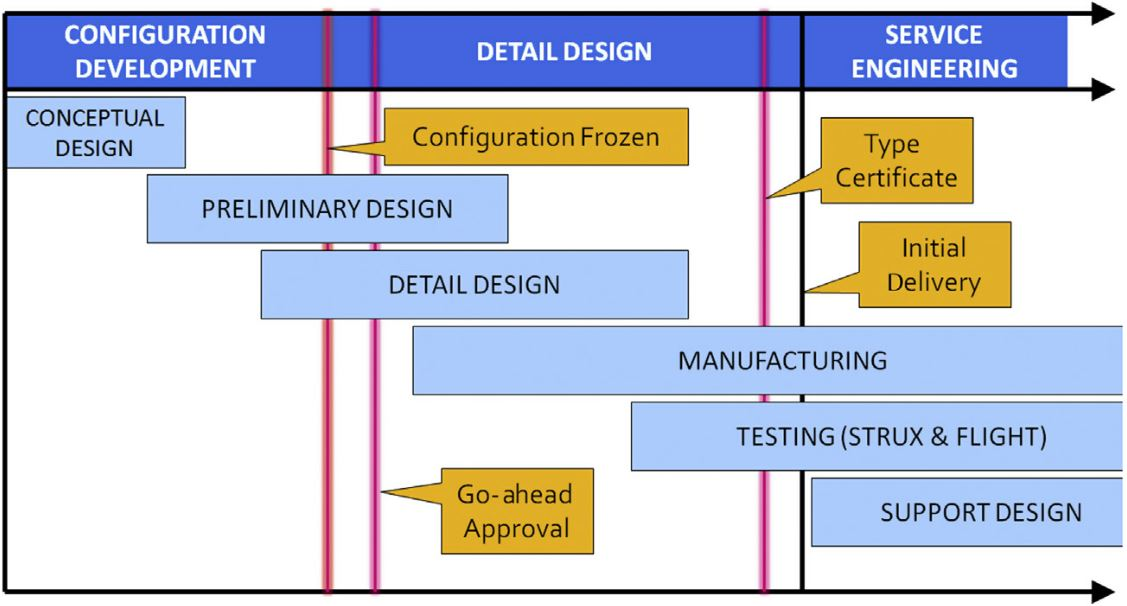
\includegraphics[height = 6 cm ]{Immagini/Process_Design_Torenbeek}
\caption{Aircraft design process for Torenbeek (\num{1986}).}
\label{fig:2}
\end{figure}


\section{Design Requirements and Objectives of an Aircraft}

The general design objective of a transport aircraft is to transport a payload over a distance between airports  against minimum costs (i.e. at an optimum speed).
So, in the design of an aircraft there is never a right answer only a best answer at a point in time. The reason is that the design of an aircraft is a balance between the following competing requirements:

\begin{itemize}
\item {\bfseries Technical.} Performance, survivability
\item {\bfseries Signature.} Survivability, appearance
\item {\bfseries Economic.} Cost, LCC
\item {\bfseries Political.} Policy, payback, risk, and so on
\item {\bfseries Schedule.} When needed? The need to be first to market
\item {\bfseries Environmental.} Limited energy source, noise, hydrocarbon emissions
\end{itemize}

Also, the priorities of these requirements change with time. An aircraft might be designed to certain technical and economic requirements, but if the government administration changes, then the priority requirement becomes political or environmental. The advice to the designer is to remain flexible and develop as robust a design as possible so that it will survive as the requirements change over time. The watchwords are compromise, balance, and flexibility.

\begin{figure}[H]
\centering
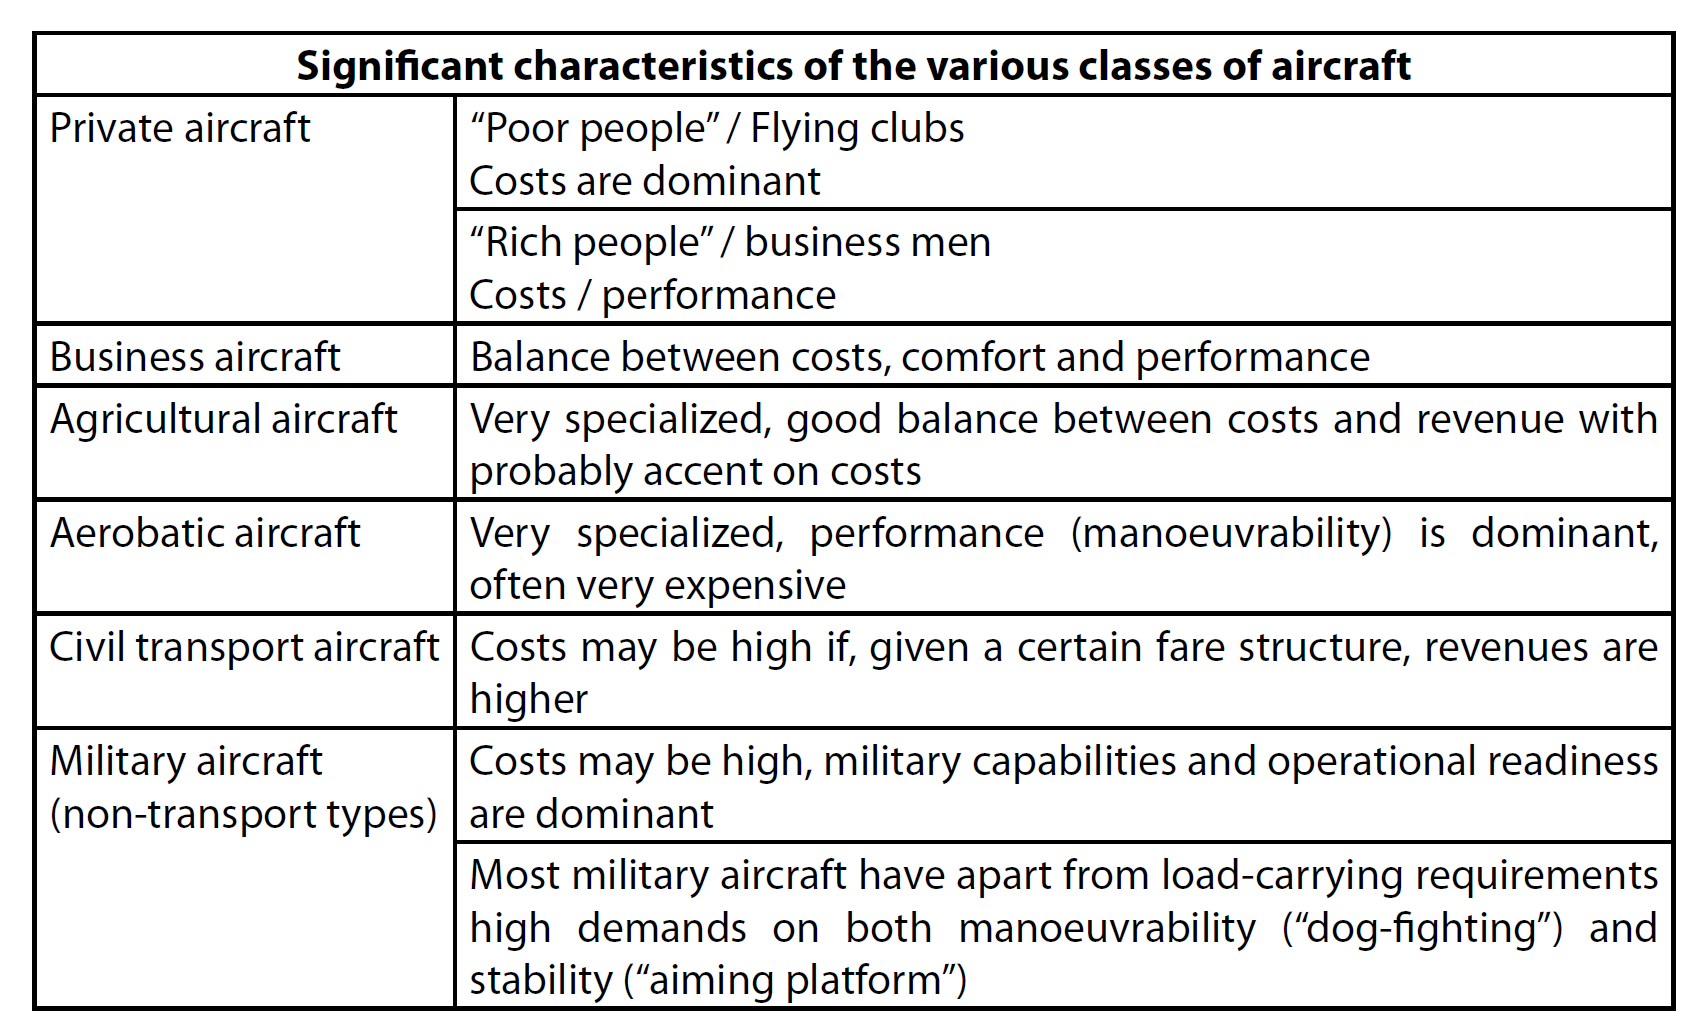
\includegraphics[height=7.9cm]{Immagini/tradeoff}
\caption{Main design requirements of various aircraft categories.\cite{obert2009aerodynamic}}
\label{introduction}
\end{figure}

An aircraft comprised of several major components. It mainly includes wing, horizontal tail, vertical tail, fuselage, propulsion system, landing gear and control surfaces. In order to make a decision about the configuration of each aircraft component, the designer must be fully aware of the function of each component. Each aircraft component has inter-relationships with other
components and interferes with the functions of other components. 

\begin{figure}[H]
\centering
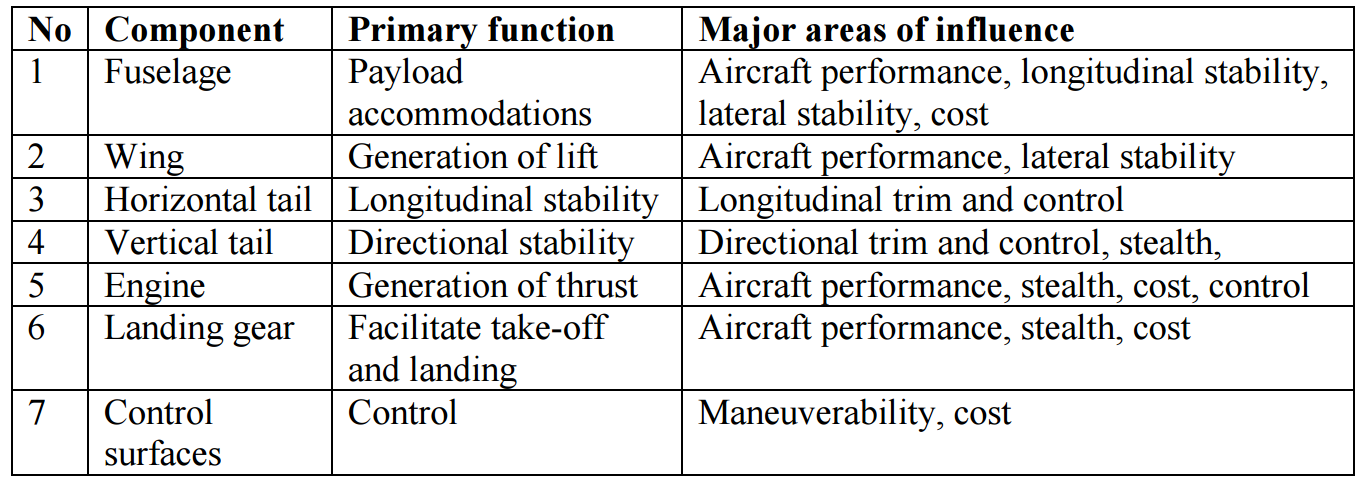
\includegraphics[height=4.9cm]{Immagini/componentfunction}
\caption{Aircraft major components and their functions.\cite{aircraft}}
\label{comp}
\end{figure}

\section{Aircraft Design Optimization}

At the beginning of the aircraft design history, optimization was limited to relatively superficial investigations to study the effects of varying a few major design parameters. 
Since the 1970s, there has been a tremendous expansion of optimization strategies and algorithms supporting advanced designers. The introduction of automated optimization has enabled designers to go into much greater in depth and fidelity of analysis than before. Synthesis programs effectively connecting the inputs and outputs of the functional group disciplines by means of an automatic control logic have been developed at aircraft manufacturers, research establishments and academia. Sophisticated computer assisted design (\gls{acr:cad}) systems for defining three-dimensional body geometries and computer graphics tools for rapidly preparing parametric surveys are available at a modest cost.\\
There are several options available to an aerodynamicist to obtain the best possible solution for a design problem. In general the optimization is an iterative process control system which interprets numerical results and then iteratively assesses variables to seek the global optimum of an objective function. In the aircraft design context, the objective function is used to decide which configuration is considered the best combination of design variables.\cite{torenbeek2013advanced} \\
It is emphasized frequently that optimization of individual goals through separate design considerations may prove counterproductive and usually prevents the overall (i.e., global) optimization of ownership cost.  \gls{MDO} offers good potential but it is not easy to obtain global optimization; it is still evolving. In a way, global  \gls{MDO} involving many variables is still an academic pursuit. Industries are in a position to use sophisticated algorithms in some proven areas. An example is reducing manufacturing costs by reshaping component geometry as a compromise – such as minimizing complex component curvature. The compromises are evident in offering a family of variant aircraft because none of the individuals in the family is optimized, whereas together, they offer the best value.\\
\begin{figure}[H]
\centering
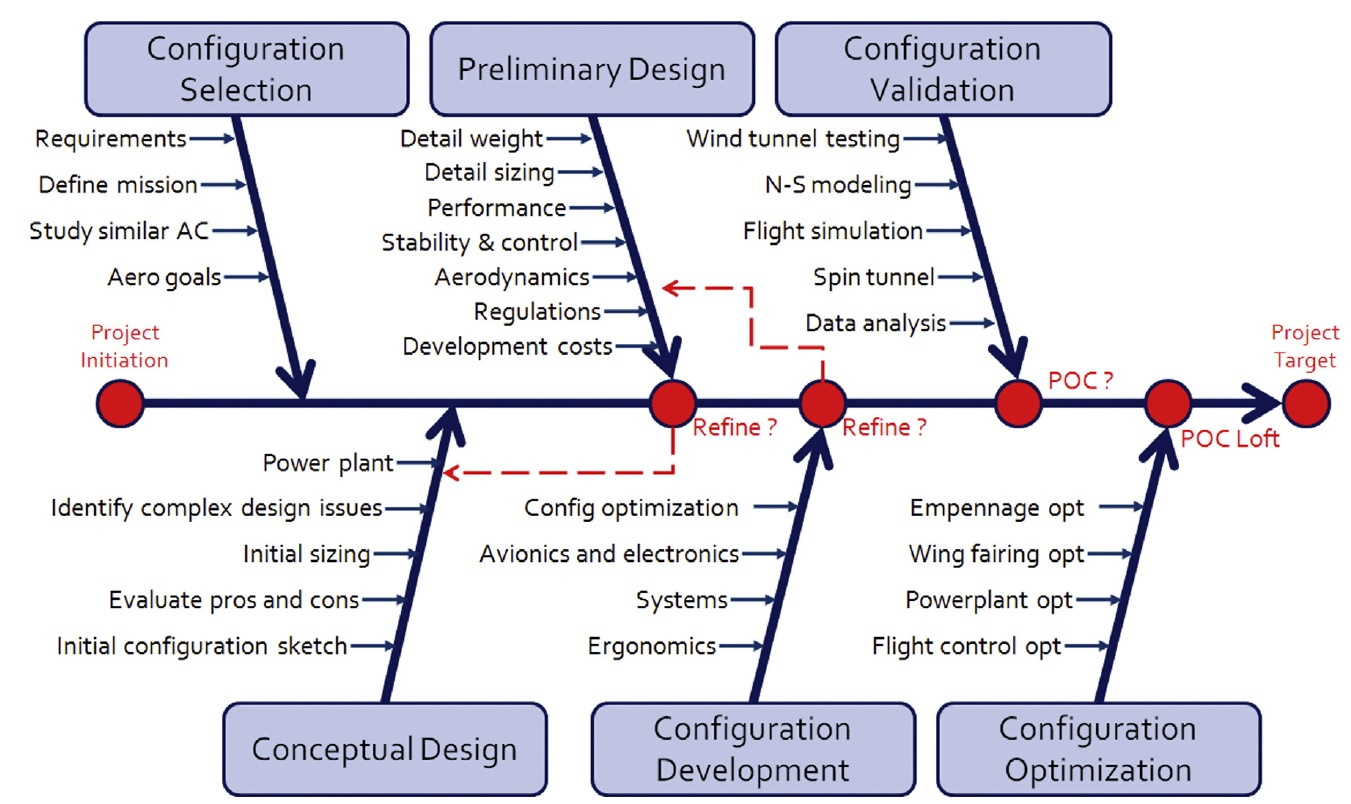
\includegraphics[height=7.6cm]{Immagini/Fishbone}
\caption{A typical fishbone diagram.}
\label{comp}
\end{figure}

According to \cite{howe2000aircraft}, the optimisation of the configuration of the aircraft within the constraints imposed by the specification is an essential feature of the project definition process. Optimisation implies that the proposed design concept not only meets the specification, but does so when a target criterion has been imposed, usually the minimisation of mass or some aspect of costs.
%
The basis of optimisation is a comparison of different design concepts and configuration variations within a given concept to determine the one which best meets the specification. Broadly the process is undertaken at two levels.
%
\begin{itemize}
\item \textbf{Concept/configuration studies} At this level alternative concepts and configurations are investigated to establish the one which would seem best suited to meet the requirements. For example a military combat requirement might possibly be met by aircraft of conventional tail, foreplane or tailless layout. Mostly the configuration of transport aircraft is well established. This phase of the study may be included at the feasibility level.
\item \textbf{Parametric studies within a given configuration} At this level the dominant parameters are varied to ascertain the best combination of them. These parameters include such items as wing geometry determined by aspect ratio, sweep, taper and thickness as well as variations in fuselage layout, powerplant installation and so on. The benefits of selecting near optimum values of certain parameters are "traded-off" against the implied penalties
imposed upon other parameters. The parametric studies may be commenced during feasibility investigations and certainly form a major part of the project definition phase. The two fundamental design characteristics which drive the parametric studies are:
\begin{itemize}
\item Wing loading, that is wing area as a function of take-off mass or weight
\item Thrust or power loading, defined as the ratio of the basic powerplant to the aircraft mass or weight
\end{itemize}
\end{itemize}
\noindent \\



\chapter{Application overview}
\label{ch:applicationoverview}
\markboth{Application overview}{}

\begin{flushright}
	{\smaller
		\textit{I do not fear computers. \\ I fear the lack of them.}\\
		--  Isaac Asimov}
\end{flushright}
In this Chapter an overview of the \gls{acr:Adopt} software, and its reference library \gls{acr:Jpad} will be presented.
\gls{acr:Adopt} is a Java-based desktop application developed at the University of Naples Federico II, conceived as a fast, reliable and user friendly computational aid for aircraft designers in the conceptual and preliminary design phases. The ultimate goal of such a tool is to perform a parametric, multi-disciplinary analysis of an aircraft and then search for an optimized configuration. The search domain boundaries are usually defined by the user through a set of specifyed parameters. An important design requirement of  \gls{acr:Adopt} is related to its interoperability with other engineering analysis tools. In fact, the application can be easily integrated into a comprehensive aircraft optimization cycle. This is made possible because  \gls{acr:Adopt} can be launched both in \gls{acr:gui} and command line mode. Much care has been given to input/output and configuration files to increase the possible uses of the software.

\begin{figure}[H]
	\centering
	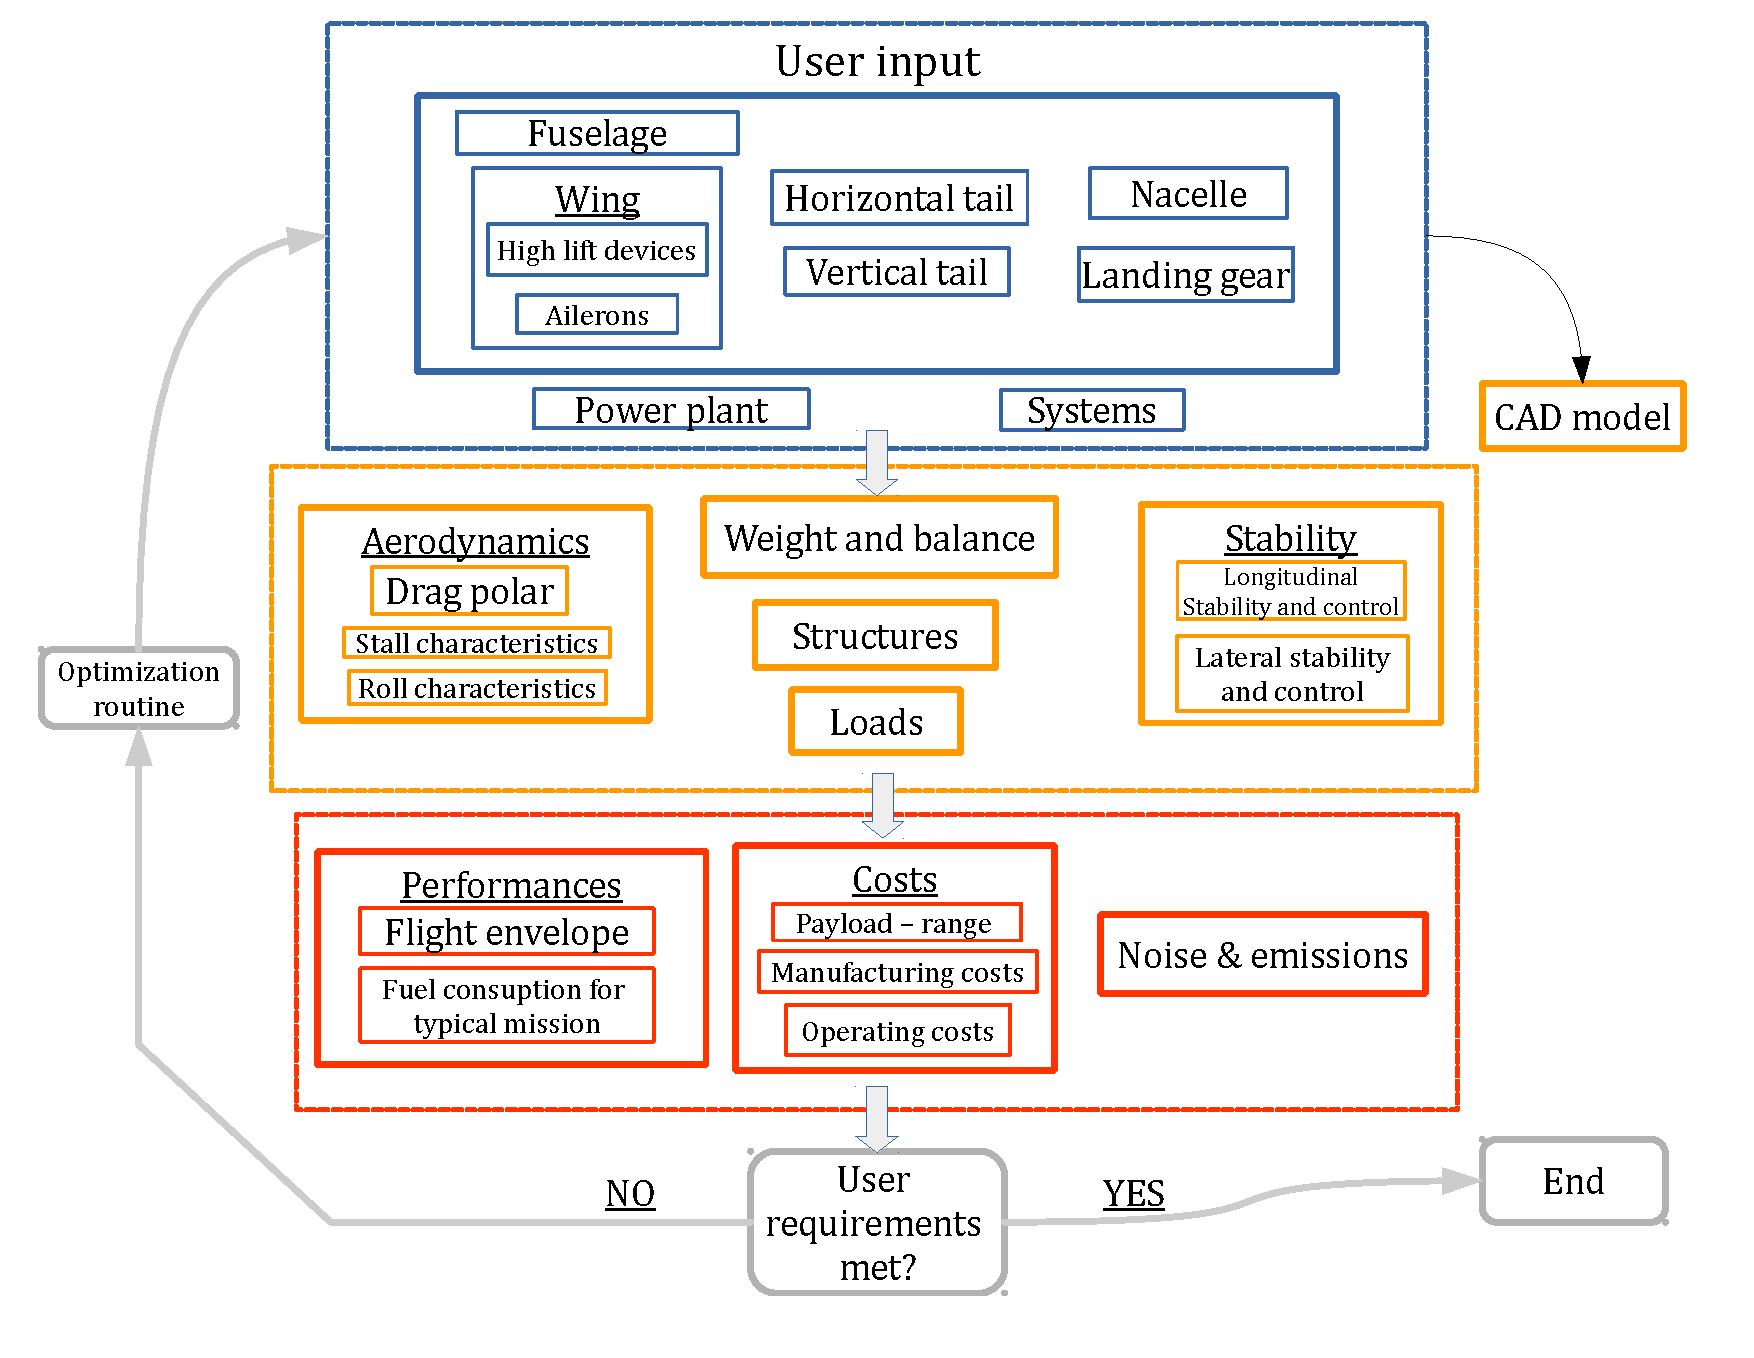
\includegraphics[height = 8.6cm ]{Immagini/flowchart3}
	\caption{Software calculation modules.}
	\label{fig:guiStart}
\end{figure}

\section{Software architecture}

\gls{acr:Jpad} library is actually divided into three package: JPADConfigs, JPADCore and JPADSandbox.  Each package is organized in several classes or more package in order to have a clear and simple classification. The possibility to place similar classes in the same package has been extensively exploited for the same reasons, see section A.2.   The source code has been extensively commented following Javadoc practices. This enabled us to automatically generate documentation using Doxygen \cite{doxgen}

\begin{figure}[H]
	\centering
	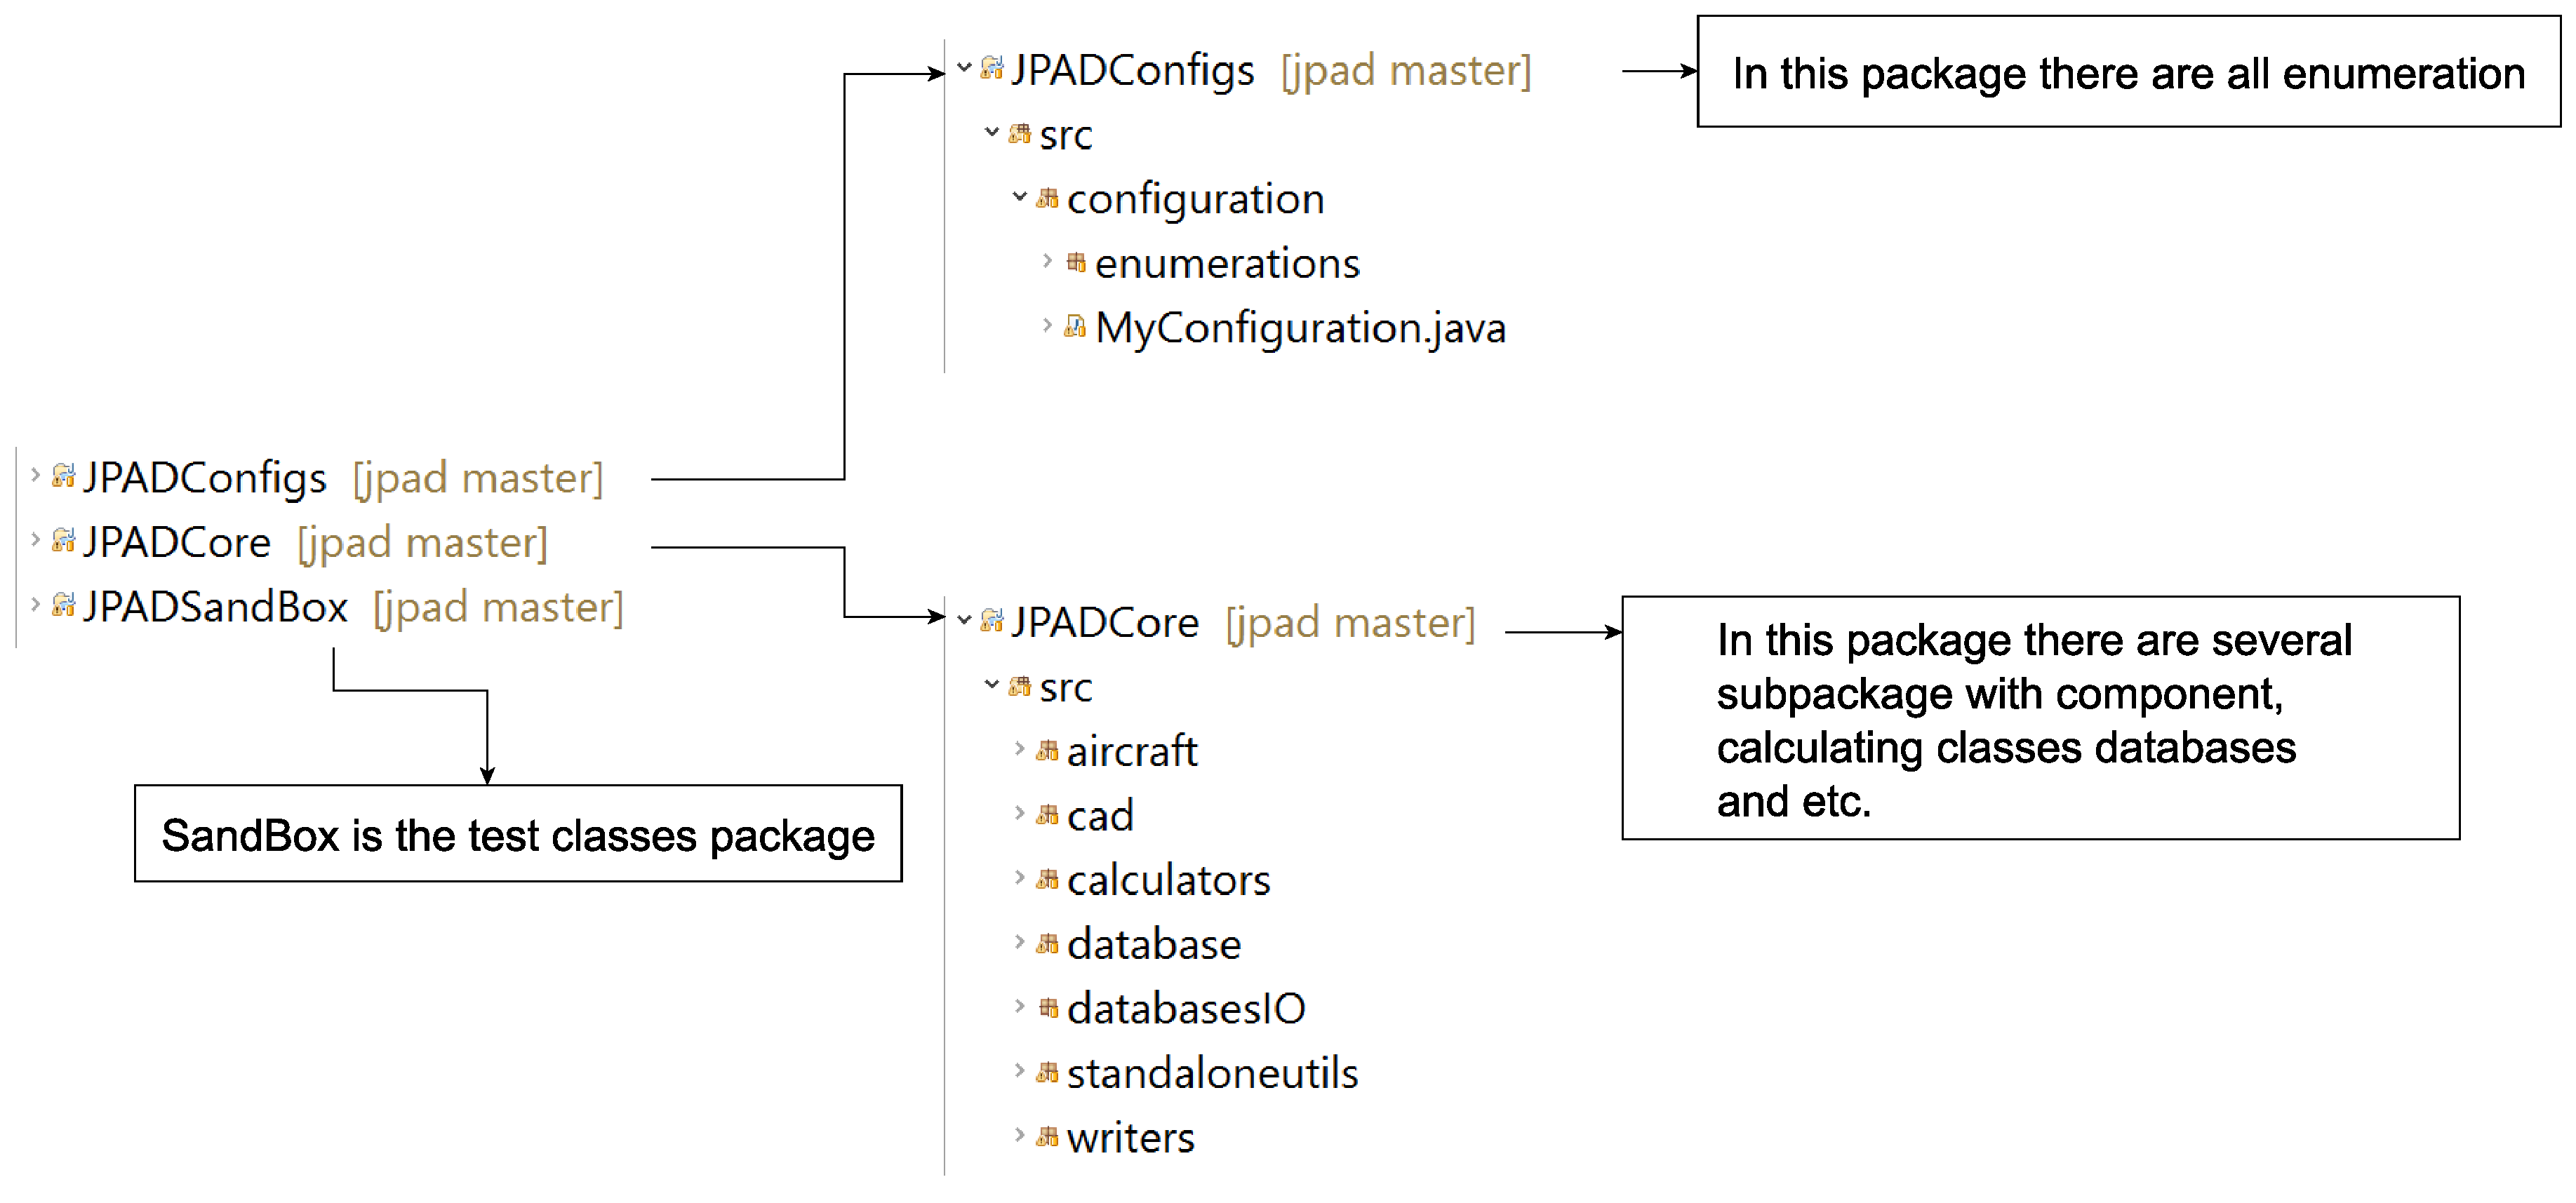
\includegraphics[height = 7.6cm ]{Immagini/organization}
	\caption{Software package division.}
	\label{fig:sw}
\end{figure}
 
 The main package of \gls{acr:Jpad} library is JPADCore where there are all aircraft component, the managers of calculator and  its computers classes. In the following subsection will explained the main features of JPADCore.\\
 JPADCore contains the following sub-packages:
 \begin{enumerate}
 \item \texttt{aircraft} $\rightarrow$ This package contains all aircraft's component classes, their calculators and the related managers and also the operating condition's class.
 \item \texttt{cad} $\rightarrow$  This package contains everything concerning the creation of CAD model.
 \item \texttt{calculators} $\rightarrow$ In this package there are the classes, divided in package by type of analysis, whose methods implement the calculation formulas.
 \item \texttt{database} $\rightarrow$ This package contains the classes that manage the database .h5 whose data are useful for the analysis. 
 \item \texttt{standaloneutils} $\rightarrow$ In this package there are several calculation classes with mathematical tools to support the analysis.
 \item \texttt{writers} $\rightarrow$ this class is in charge of writing files.
 \end{enumerate}
 
 \noindent \\
 Following will be explained the main features of the fundamental packages.
 
 \subsection{\texttt{Aircraft }package}
 Each component (e.g., the fuselage, the wing, the engine) is therefore defined in its own class. In the aircraft package there are other sub-package for components. In each of these there are a class for the object definition and a manager for the analysis. These manager classes uses the utilities located in the calculator package. \\
 The sub-package in the \texttt{aircraft} package are the following:
 
 \begin{itemize}
 \item \texttt{Auxiliary} that manages the airfoils
 \item  \texttt{Component} that contains the \texttt{aircraft} class, the aircraft components packages (fuselage, lifting surfaces, nacelles, power plant, fuel tank, landing gear, systems) and, inside them, their manager analysis classes used to call related analysis methods. 
 \item \texttt{OperatingConditions} 
 \end{itemize}

The main aircraft components are organised as follows: \\ 

Basic data for describing the {\bfseries fuselage} are contained in the \texttt{fuselage} class. This holds all the fuselage overall properties, such as the length, maximum width and maximum height, length ratios between the nose and the tail parts length to the constant section part length, number of decks and so on. Other classes in the package manage the shape of fuselage sections and outlines (which define the fuselage shape in the xz and xy planes) and aerodynamics calculations (Aerodynamics class).\\ \\

The data relating to the {\bfseries lifting surfaces} are contained in the \texttt{liftingSurface } class. Since the lifting surfaces of an aircraft share several characteristics, a single class has beencreated to manage the wing, the horizontal and vertical tail and, eventually, the canard. The lifting surface specific category (that is, wing, horizontal tail etc.) is acknowledged through a \texttt{MyComponentEnum} variable which has to be specified when creating the lifting surface object. By default, a lifting surface has three primary span stations: root ($\eta = 0$), middle and tip ($\eta = 1$). The middle station location is user-defined and is used to represent a change in chord.y/ law; such a change can be due to a lifting surface kink or to the beginning of a tapered part. If the wing is simple tapered the middle station can also be omitted.\\ \\

The data relating to the {\bfseries airfoils} are handled by \texttt{Airfoil} class, that creates for each lifting surface three airfoils, located respectively at $\eta=0$, $\eta=1$ and at middle station. An airfoil object holds:
\begin{enumerate}
	\item the position along the semispan, $\eta$;
	\item twist value relative to root, $\epsilon_g$;
	\item zero lift angle of attack, $\alphazlp$;
	\item angle of attack value at the end of the linear part of $C_l(\alpha)$ curve, $\alphastar$;
	\item stall angle of attack, $\alpha_{stall}$;
	\item lift gradient of the linear part of $C_l(\alpha)$ curve, $\Clalphap$;
	\item minimum drag coefficient, $C_{d,min}$;
	\item lift coefficient at $C_{d,min}$, $C_l@C_{d,min}$;
	\item lift cofficient at the end of linear part;
	\item maximum lift coefficient, $\Clmaxp$
	\item drag polar $K$ factor;
	\item aerodynamic moment coefficient gradient, $C_{m_\alpha}$;
	\item aerodynamic center x coordinate, $x_{ac}$;
	\item aerodynamic moment coefficient with respect to the aerodynamic center, $C_{m_{ac}}$ or $\Cmzerop$;
	\item aerodynamic moment coefficient with respect to the aerodynamic center at stall, $C_{m_{ac},stall}$;
	\item maximum thickness to chord ratio, $t/c_{max}$;
	\item x,z non dimensional coordinates.
\end{enumerate}
At the time of writing all these quantities have to be entered by the user. The \texttt{Airfoil} class provides the \texttt{populateCoordinateList()} method which transforms the non dimensional coordinates provided by the user in order to obtain their actual coordinates, which takes into account of actual chord length, ACRF position, sweep, twist and dihedral.\\ \\

The  {\bfseries power plant} is defined in the package \texttt{PowerPlant} in \texttt{components}. In this package there is the \texttt{engine} class that initializes the data related to the single engine. An other class in the same package, \texttt{powerPlant} creates the parametric model of the power plant using a list of objects creates by \texttt{engine}.


\subsection{\texttt{MyOperatingConditions} class}
As the name suggests, this class contains all the data related to atmosphere conditions (which are currently derived from altitude value using the 1976 ISA model), current speed (Mach number), gravitational acceleration (\SI{9.80665 }{\meter/\second^2}) and sea level pressure (\SI{101325}{\Pa}).

A \texttt{MyOperatingConditions} object can be created regardless of the aircraft configuration as the class is entirely self contained: the aircraft could also be undefined at the time of the object creation. If the user wants to run several analysis at different operating conditions, a \texttt{MyOperatingConditions} instance has to be created for each one.

\subsection{\texttt{CAD} package}

Throughout the development of the application, great care has been given to the making of the CAD model for several reasons:
\begin{itemize}
	\item it enables the user and the user developer to have an immediate feedback about the data provided to the application: if some geometrical parameter is wrong, the CAD model makes it impossible not noticing it;
	\item it allows the user to run a CFD analysis with an external program. The CAD model has been in fact built so that it is ready to be meshed by an external mesher without any further adjustment;
	\item it provides an accurate estimate of the wetted surface of each component.
\end{itemize}

The creation of the CAD model was made possible by the occjava library, whose classes and methods have been used to build each component's model.

 \subsection{\texttt{Calculators} package}
 This package includes all the calculators classes. Calculator classes have been created to evaluate quantities related with more than one component. The calculator classes are the following:
 
 \begin{itemize}
 \item {\texttt{aerodynamics} package}
\item {\texttt{cost} package}
\item {\texttt{geometry} package}
\item {\texttt{performance} package}
\item {\texttt{stability} package}
\end{itemize} 

Each of these package contains calculators classes and concerning methods that implement all mathematical equations. These methods are called by the analysis manager classes that are in the package of relatives components (such as fuselage, lifting surfaces etc.).

\subsection{\texttt{Database} package}
In order to manage a large quantity of data, it has been necessary to read data from graphs available in literature; for such a reason an extensive database has been built over the years by several of my colleagues to digitalize this data in order to exploit it in a computer program. The data has been stored in an hdf5 file.\\
In the \texttt{database} package there are all the classes that manage and reads the .h5 files. To obtain the useful data in JPAD, interpolating functions are used . These functions can be of one, two or three dimensions and read data from graphics that have been digitize previously.

\subsection{\texttt{Writers} package}
 This class is based on the Apache POI library and provides methods which enable the user developer to easily add a sheet to an XLS file, to set the styles of the XLS file and to compare different XLS files.The last function permits to create an XLS file which contains a different aircraft data for each column; in such a way the comparison between two or more aircraft (or,
simply, between slightly different configurations of the same aircraft) is easier and effective.



\section{Graphical User Interface (GUI)}
An extensive work has been done to set up an effective Graphical User interface (GUI) to reduce the time the user has to spend to obtain relevant results. The result presented in this section is the early step of graphical interface, which is currently in development.\\ 

The Java programming language greatly helped to build the GUI: several open source libraries (SWT, JFace) allowed us to build a functional yet pleasant GUI which allows the user to easily change the aircraft’s parameters, to view a 3D model of the defined geometry, to launch a new analysis and view the corresponding results. The current GUI appearance is shown in fig. \ref{fig:guiStart}. It is composed of several items:
\begin{enumerate}
	\item a menu bar (on top), which holds all the available actions divided in sub-categories;
	\item a toolbar (below the menu bar), which holds the most important actions needed to interact with the application. The toolbar, as the menu bar, is always visible to the user;
	\item a project tree (on the left), a key component of the GUI since it provides access to all the components of the aircraft and the analysis results any time during the execution of the application. The project tree appears once an aircraft is created and can be eventually hidden;
	\item a 3D view, which shows the CAD model of the aircraft selected by the user. The CAD model can be updated each time the user wants to check the changes made to the aircraft geometry;
	\item a log message window, placed at the bottom, that tells the user the status of pending operations. This window can be hidden;
	\item a tab folder, which contains all the windows opened using the project tree; these windows can be closed and reopened any time.
\end{enumerate}


\begin{figure}[H]
	\centering
	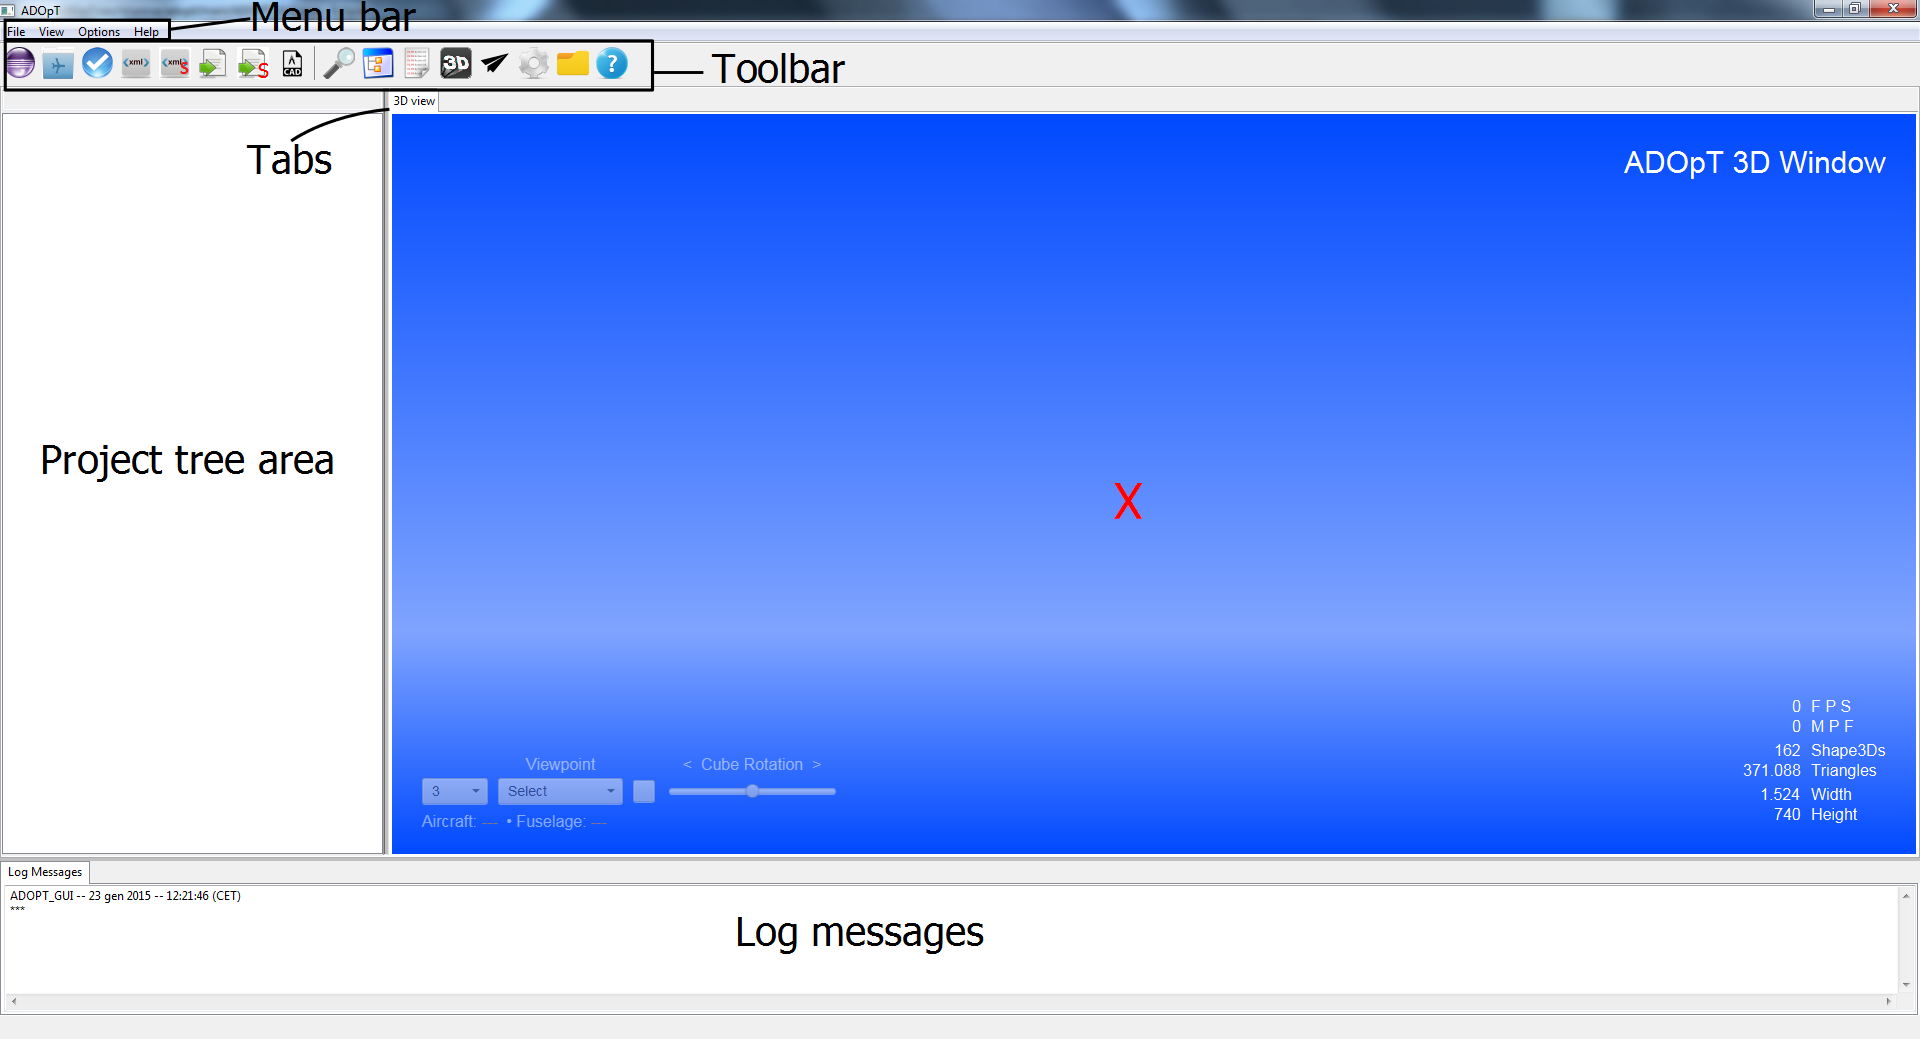
\includegraphics[height = 7cm ]{Immagini/gui/applicationStart.png}
	\caption{The GUI when the application is started.}
	\label{fig:guiStart}
\end{figure}

\subsection{Typical work session}
In developing the application we focused on making the user's typical work session as simple as possible. Few basics steps are required for running an analysis:

\begin{enumerate}
\item create a new aircraft, which we will call A. This can be done using the corresponding button \big(
\includegraphics[scale=0.6]{Immagini/gui/icons/FolderAirplane_32x32.png}\big) in the toolbar, which instantiates the default aircraft
	
\item set the parameters that define the aircraft model using the corresponding window opened using the tree
\begin{figure}[H]
		\centering
		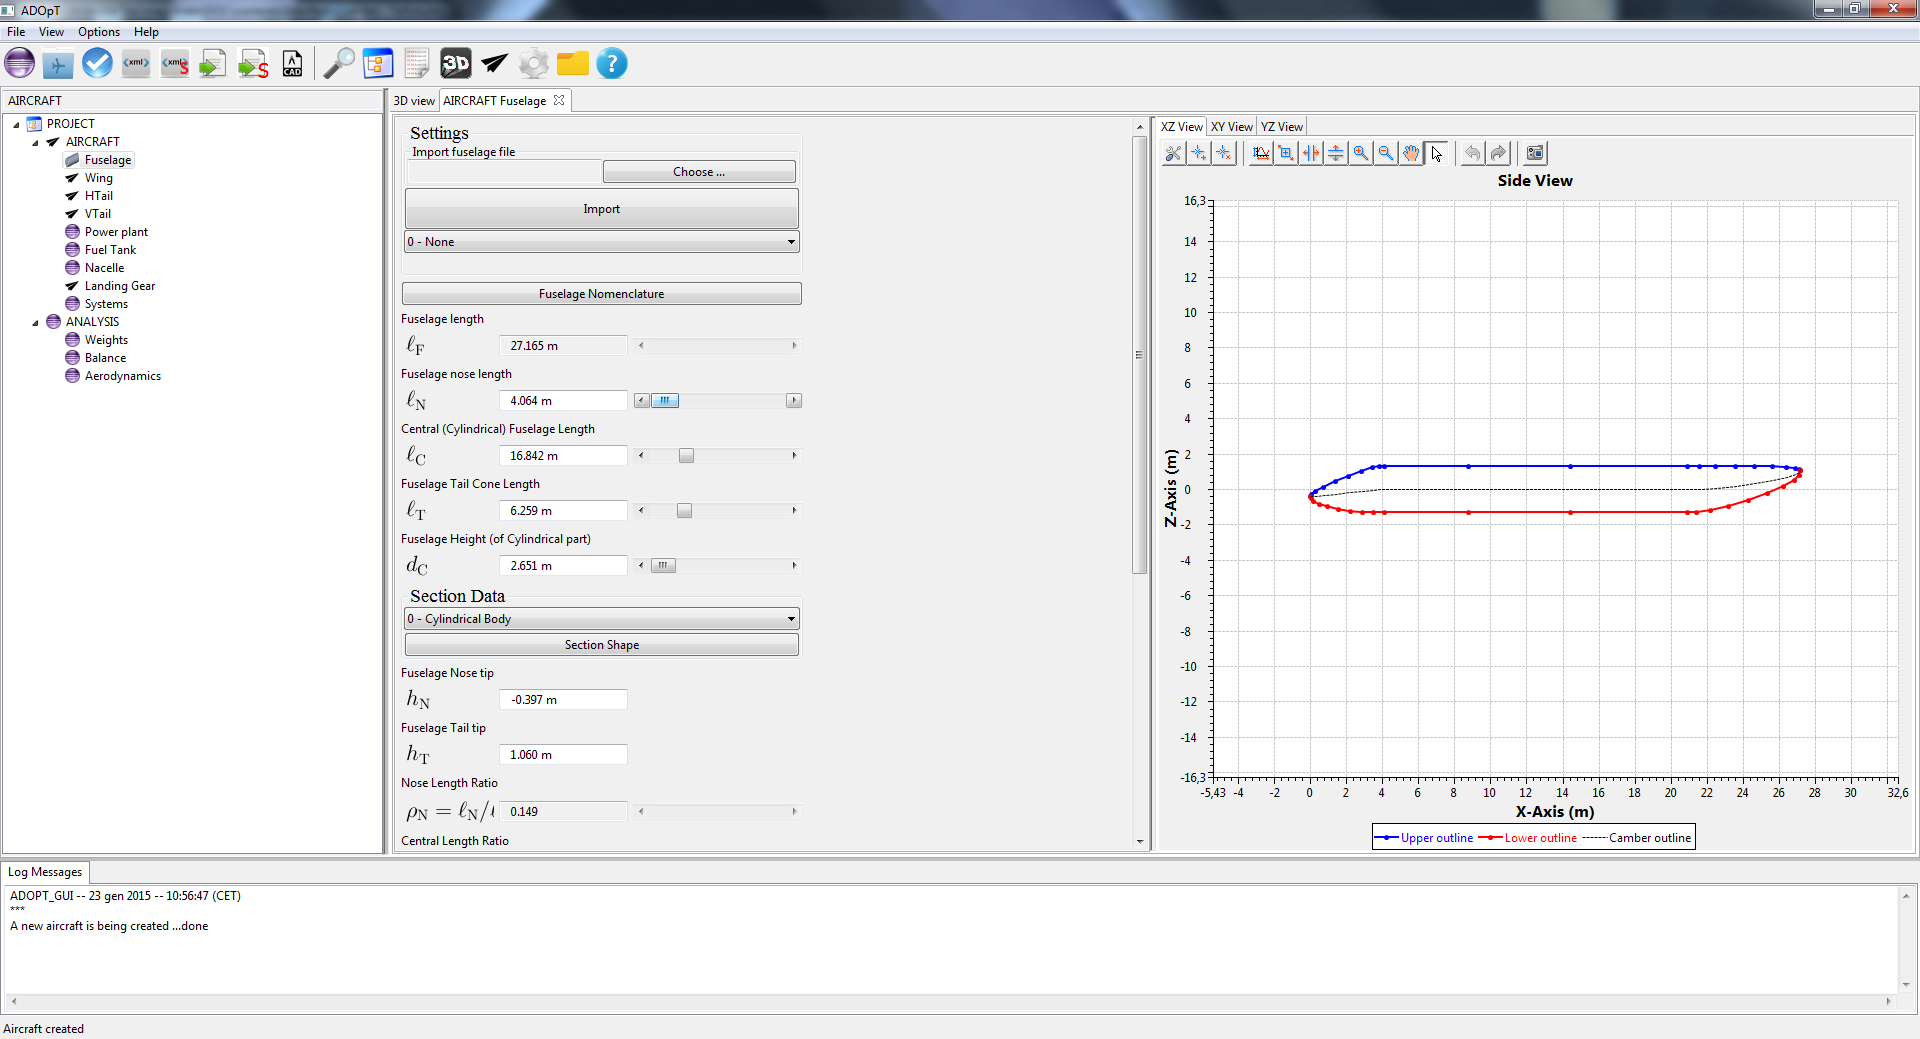
\includegraphics[height = 7cm]{Immagini/gui/changeFusParam.png}
		\caption{The window for changing the fuselage parameters.}
	\end{figure}
\item explore the 3D model \big(
\includegraphics[scale=1.2]{Immagini/gui/icons/3DView_32x32.png}\big) of the aircraft and eventually change some parameters if there is some error
		\begin{figure}[H]
	\centering
		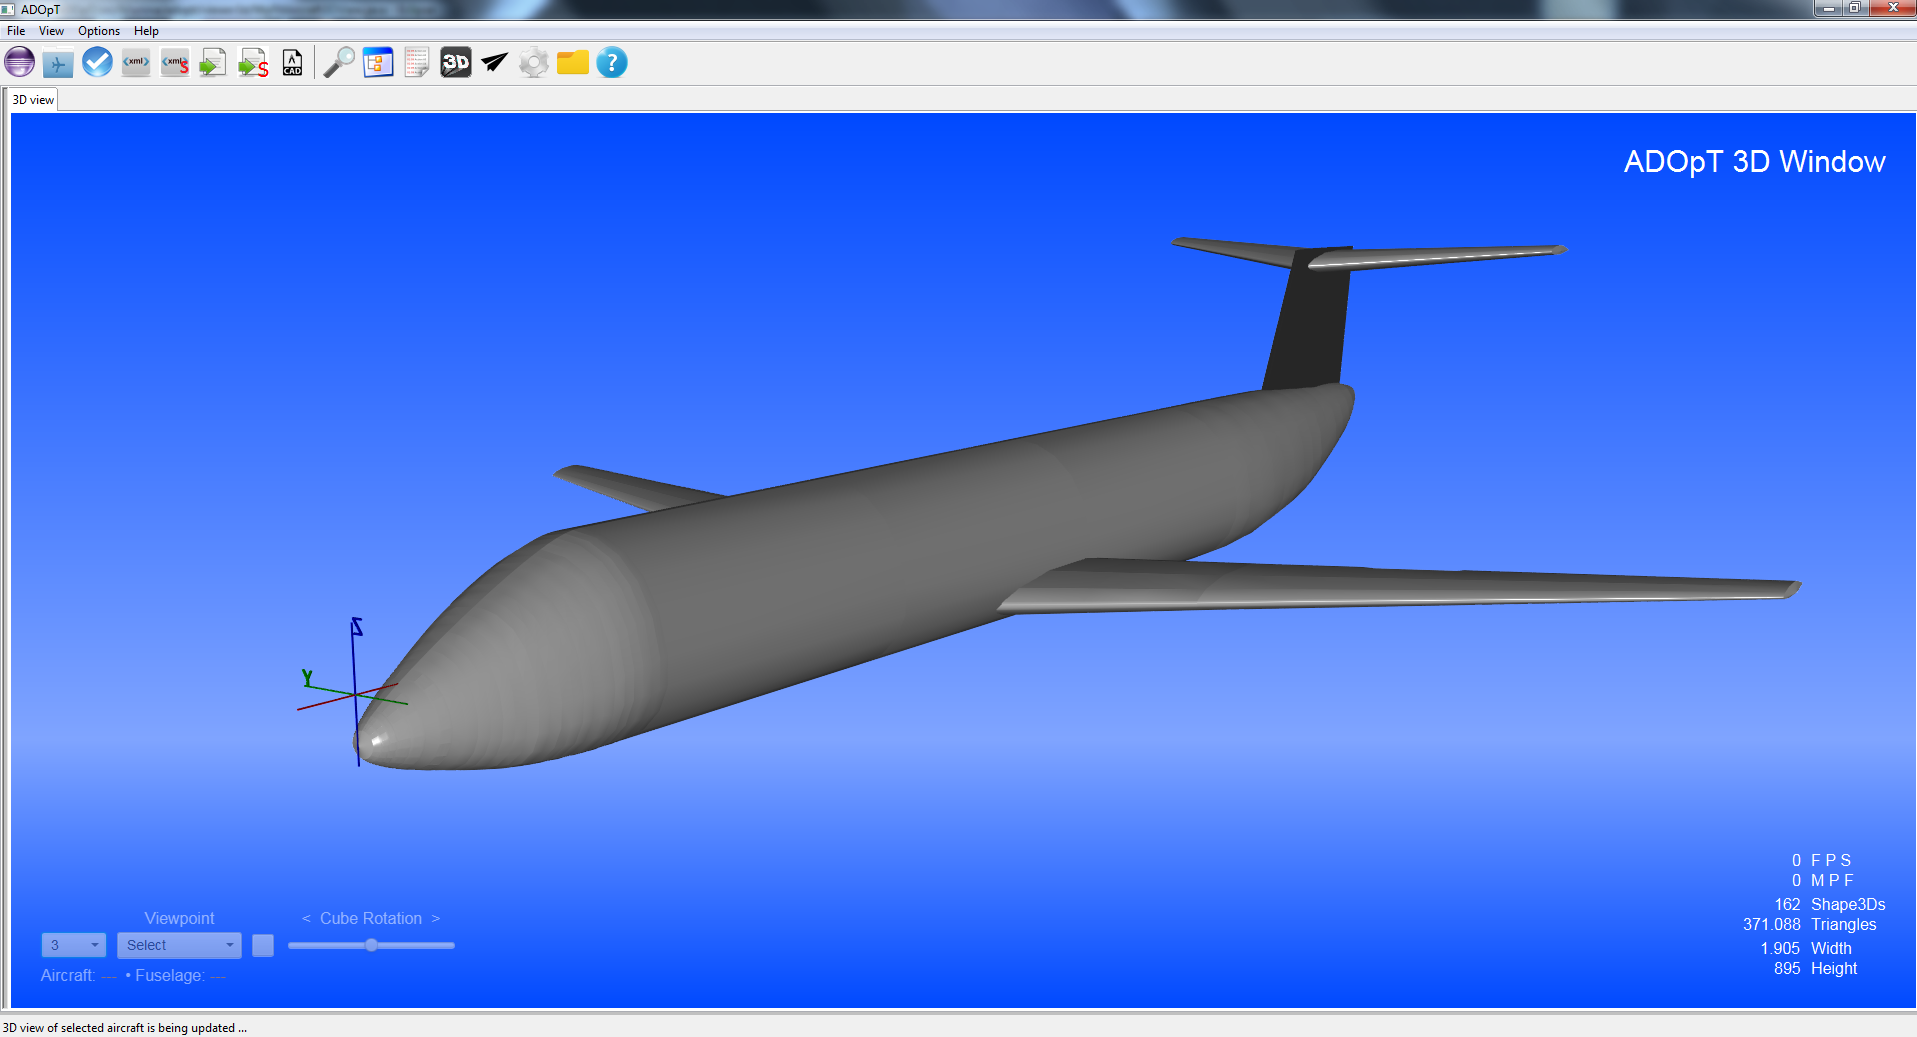
\includegraphics[height =7cm]{Immagini/gui/cad1.png}
		\caption{The aircraft 3D view (log window and project tree hidden).}
	\end{figure}
\item execute a complete analysis \big(
\includegraphics[scale=0.5]{Immagini/gui/icons/analysis_32x32.png}\big) of the aircraft previously defined;

	\item export the analysis results to an XML and/or an XLS file \big(
\includegraphics[scale=0.4]{Immagini/gui/icons/Export_32x32.png}\big);
	
	\item eventually export the CAD model of the aircraft \big(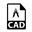
\includegraphics[scale=1.2]{Immagini/gui/icons/cad_32x32.png}\big);
	\item save the current aircraft to an XML file \big(
\includegraphics[scale=0.4]{Immagini/gui/icons/XML_32x32.png}\big).
\end{enumerate}

	
At this point the user could simply change the current configuration until the analysis results are satisfactory. The application can however help the user in finding such a configuration, since it can hold multiple configurations simultaneously, analyse all of them and compare them side by side. To accomplish this task, once the first aircraft has been created, the user should:

\begin{enumerate}
	\item import the aicraft previously saved or create an entirely new aircraft, which we will call B;
	\item change B parameters and run a new analysis on it;
	\item study the results and eventually change some of the parameters;
	\item save every configuration and the corresponding results to file;
	\item export both aircraft and the corresponding results to an XLS file.
\end{enumerate}
	
	\begin{figure}[H]
	\centering
		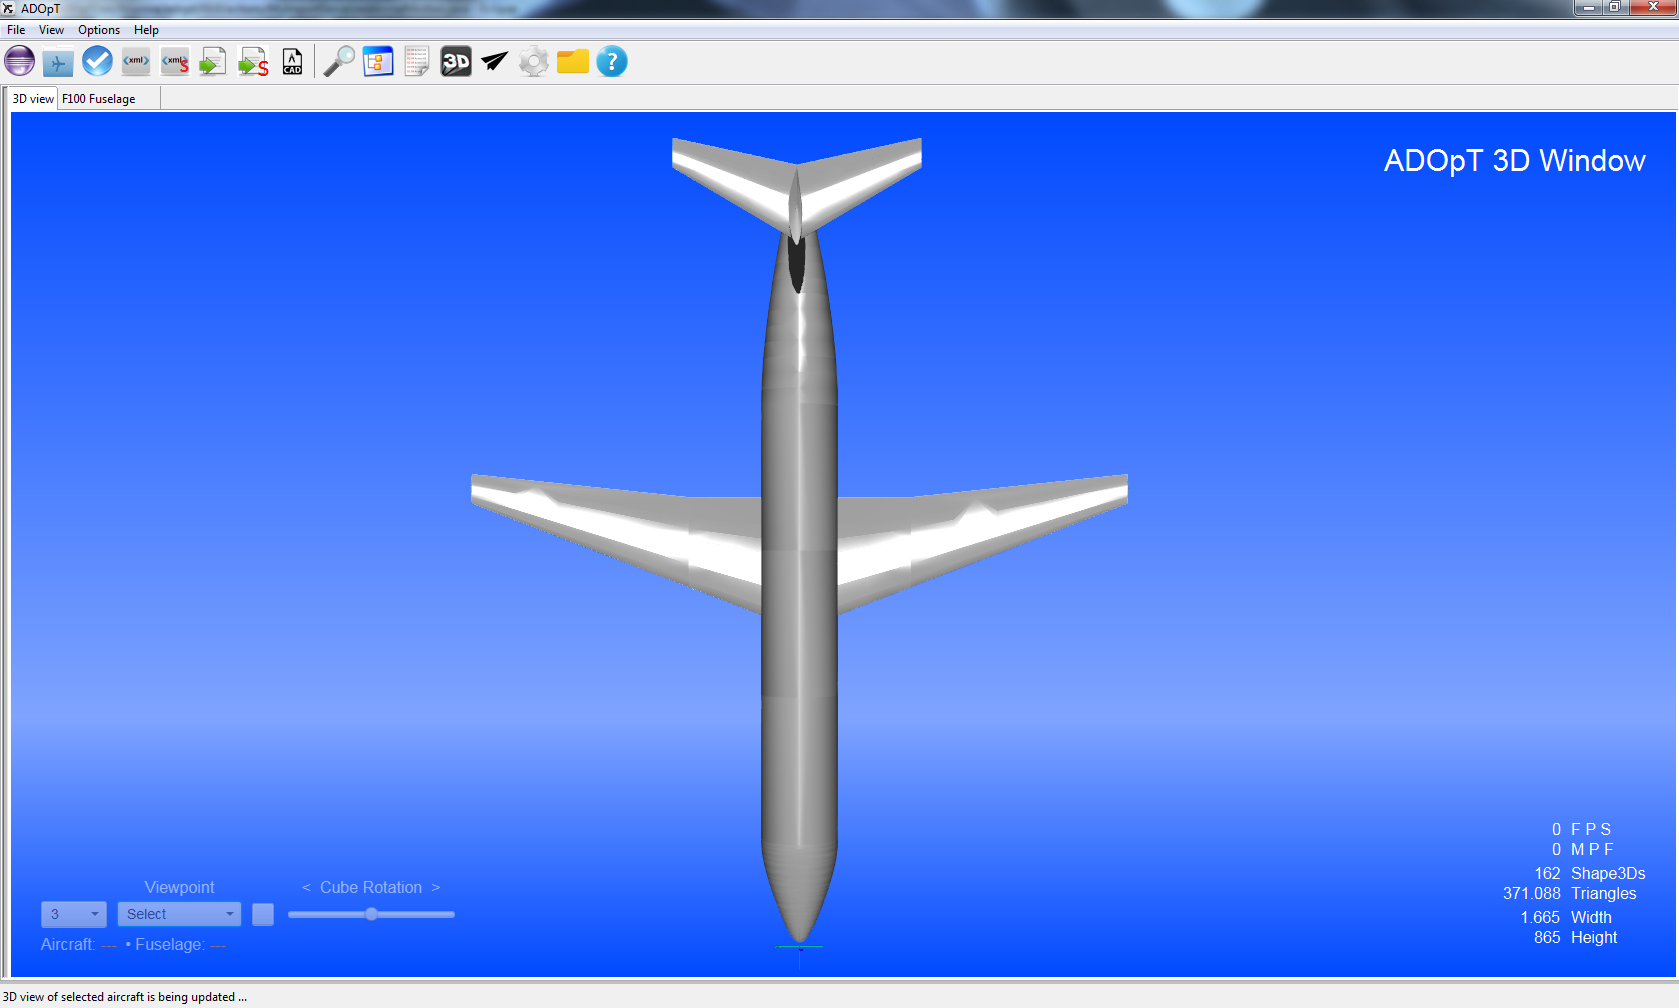
\includegraphics[height =8cm]{Immagini/gui/cad3.png}
		\caption{The aircraft 3D view.}
	\end{figure}		
%

%\begin{figure}[H]
%		\centering
%		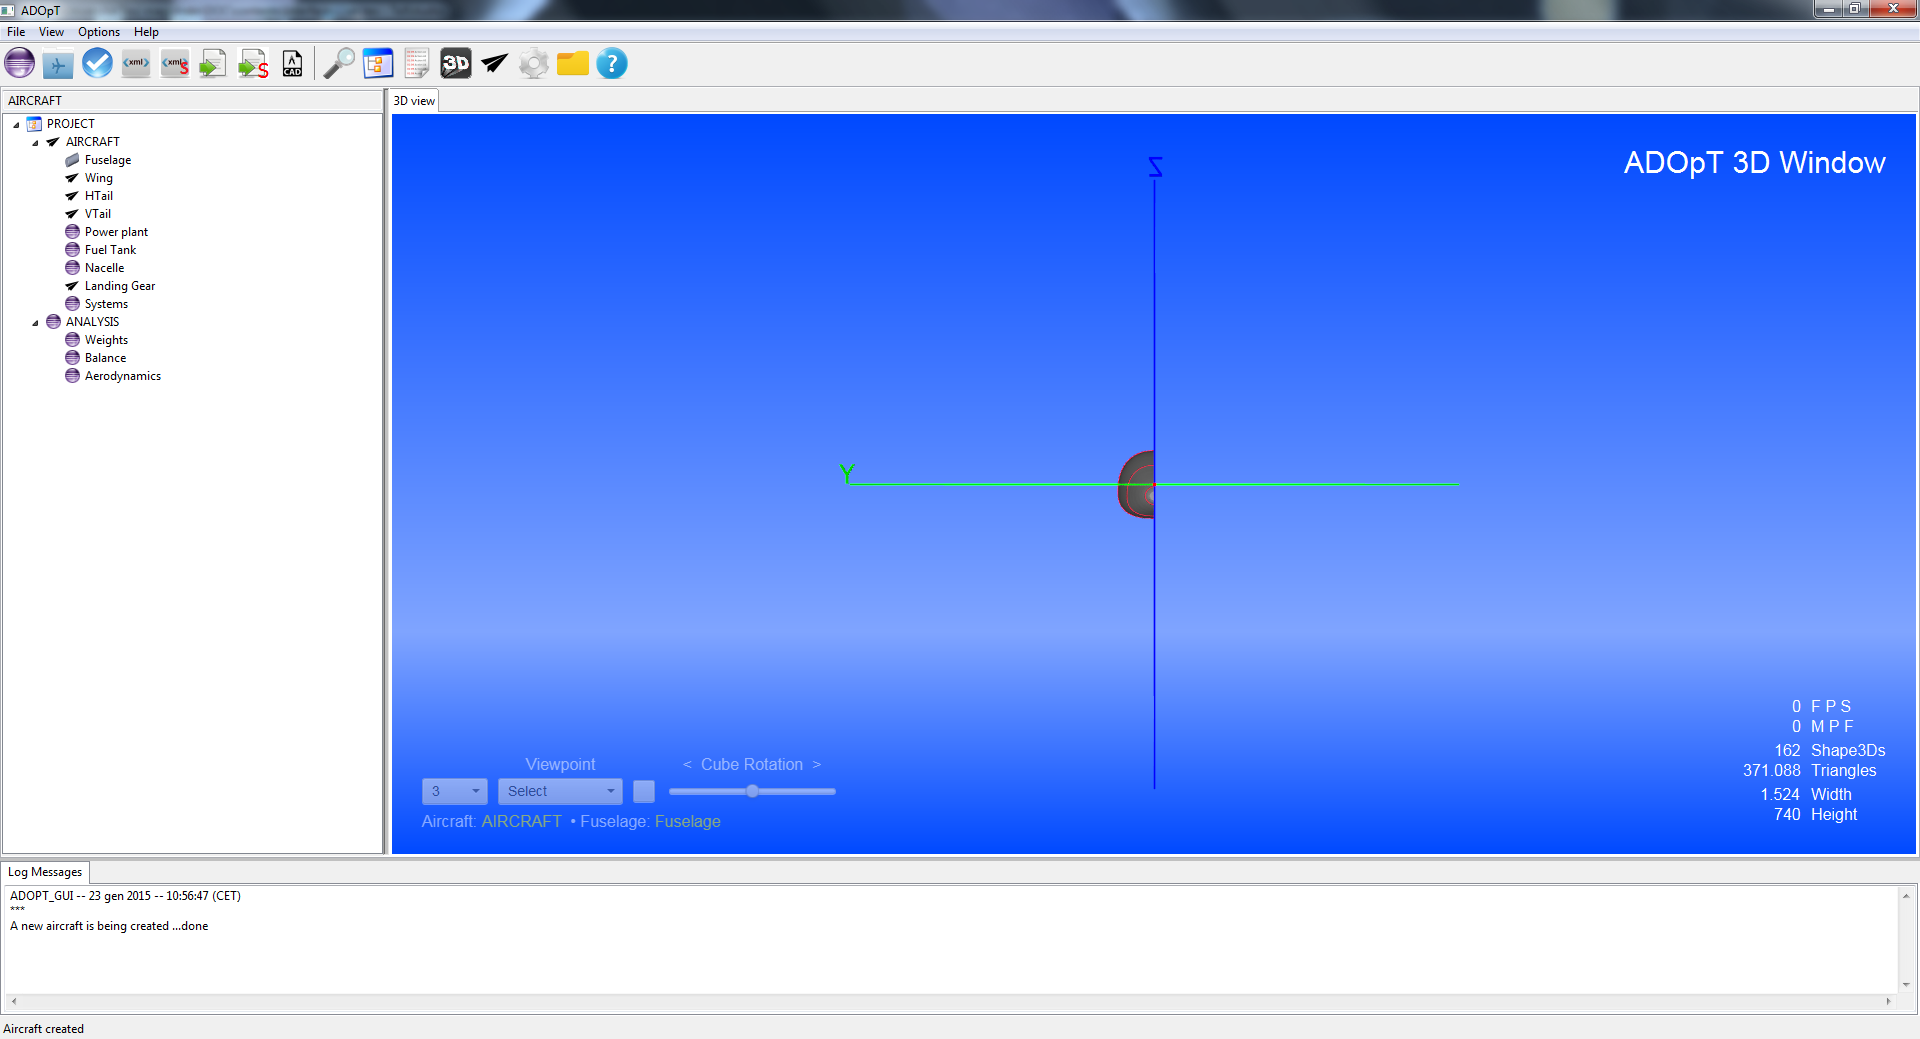
\includegraphics[height = 8cm ]{Immagini/gui/createAircraftDone.png}
%		\caption{The GUI as it appears when an aircraft is created.}
%		\label{fig:guiDescription}
%	\end{figure}


There is no limit to the number of aircraft the application can handle; each aircraft is added to the project tree as shown in fig. \ref{fig:projectTreeMulti} providing access to the corresponding components and analysis.

\begin{figure}[H]
	\centering
	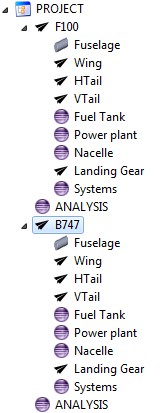
\includegraphics[height=8cm]{Immagini/gui/projectTreeMulti.png}
	\caption{The project tree holding two different aircraft}
	\label{fig:projectTreeMulti}
\end{figure}

\begin{figure}[h]
	\centering
	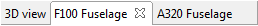
\includegraphics[width=5cm]{Immagini/gui/tabId.png}
	\caption{Same component tab belonging to different aircraft}
	\label{fig:tabId}
\end{figure}



\subsection{CAD modelling}
The application can also be used as a basic parametric \gls{acr:cad} modeler. The capability to change the aircraft parameters using the corresponding controls in the \gls{acr:gui}, coupled with the 3D view, allows the user to change each component shape and dimension, view the updated \gls{acr:cad}model and eventually export it to file once some satisfactory results have been obtained.\\
The creation of the CAD model was made possible by the occjava library, whose classes and methods have been used to build each component’s model. The CAD model can be saved in two different file formats: STEP and BREP; they have proven to take both little memory and to give the best results in terms of geometry representation. The IGES format gave instead mixed results so we preferred to use only the first two.

\begin{figure}[H]
	\centering
		\includegraphics[width=6 cm]{Immagini/gui/CADfuselageTailBAD2.png}
		\caption{A detail of the tail of the fuselage obtained as a unique loft.}
		\label{fig:badTail}
	\end{figure}
	
	\begin{figure}[H]
	\centering
		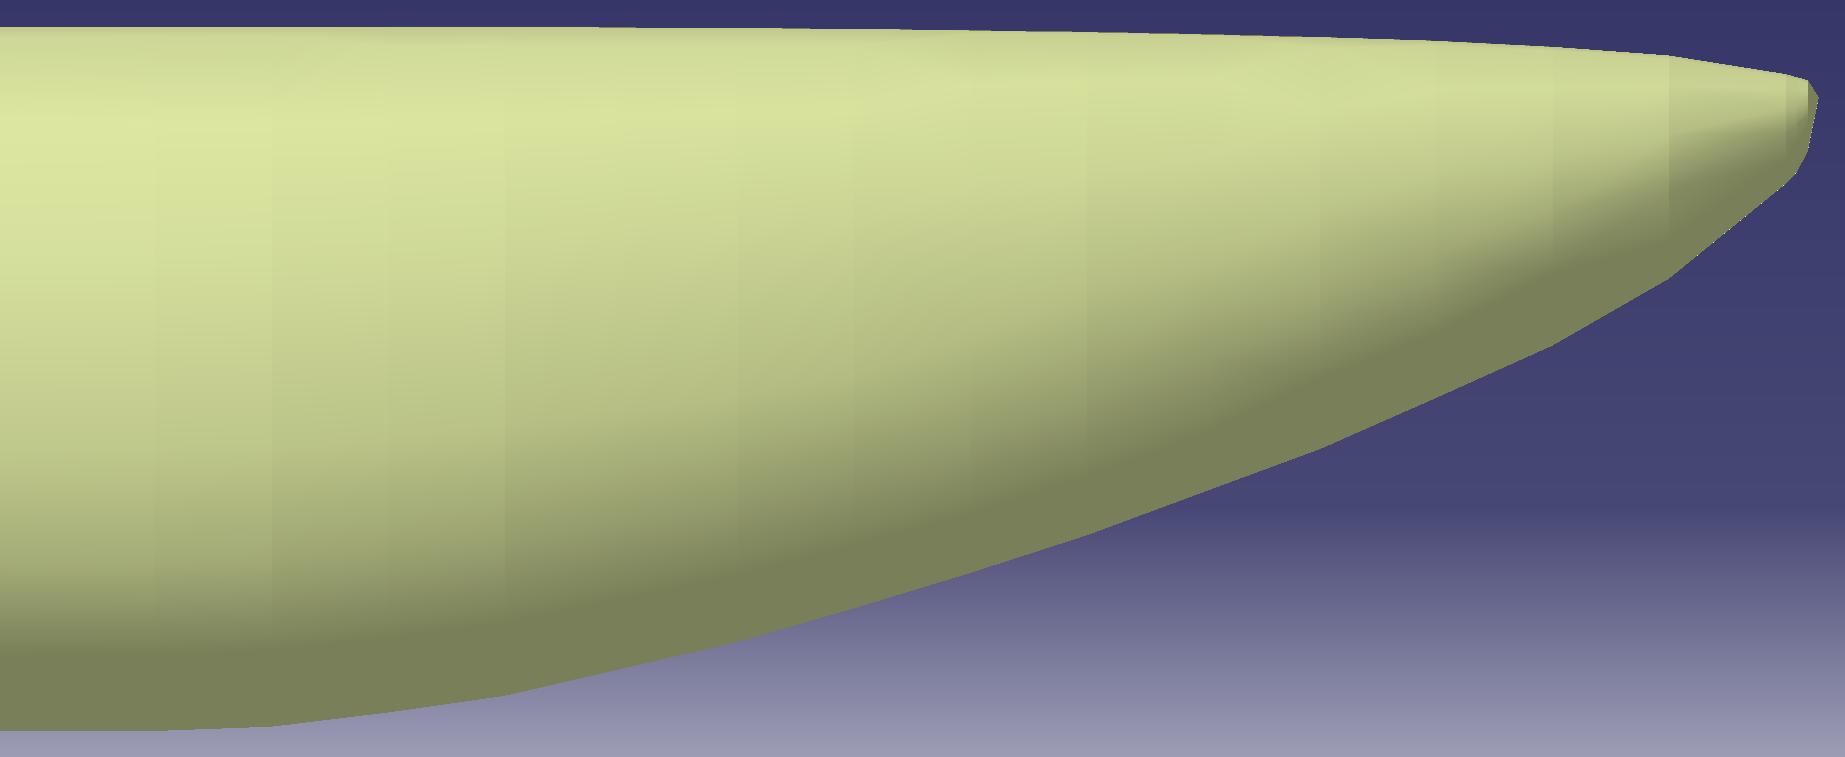
\includegraphics[width=6 cm]{Immagini/gui/CADfuselageTailOK.png}
		\caption{A detail of the tail of the fuselage obtained sewing together its parts.}
		\label{fig:goodTail}
\end{figure}


	\begin{figure}[H]
	\centering
		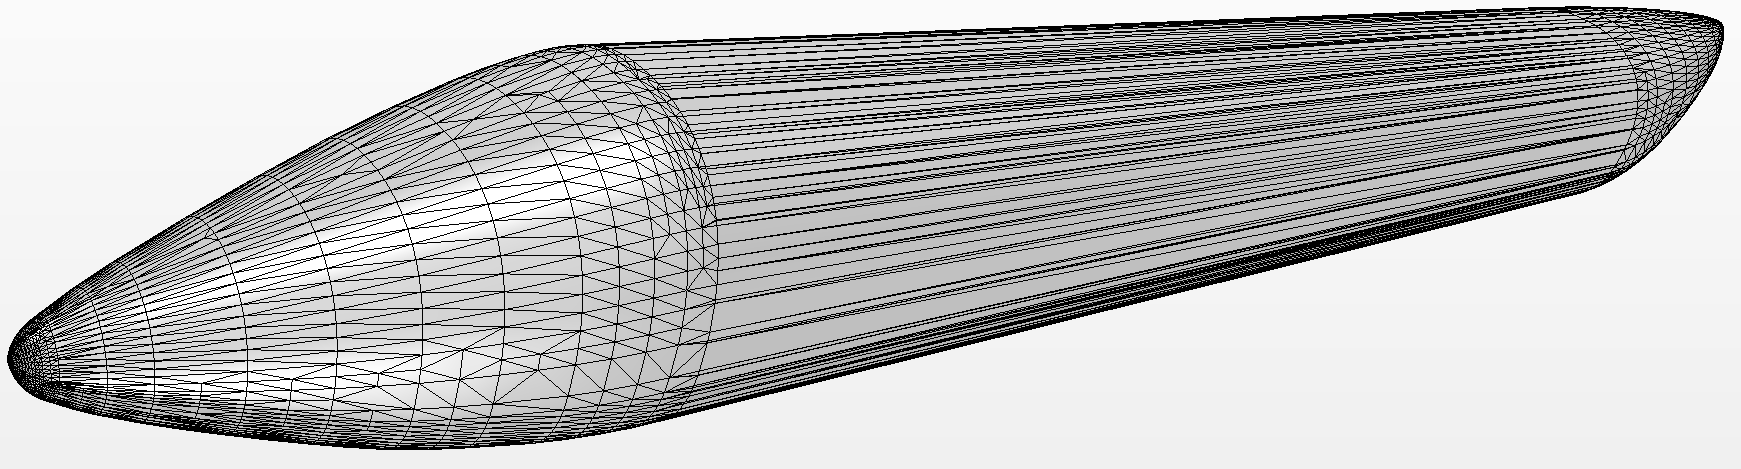
\includegraphics[width=12 cm]{Immagini/gui/CADfuselage}
		\caption{External fuselage shape exported as STEP file.}
		\label{fig:goodTail}
\end{figure}


\subsection{Interface with external software}
With ADOpT it's also possible to execute some high-fidelity analyses using external tools (i.e. CFD Navier-Stokes solver, panel method, FEM for structural static and dynamic analysis, etc.) by importing the dedicated output (such as a CAD model) produced by the software. The higher-fidelity tools could improve the results obtained and give therefore some useful clues in order to start a new design loop with different requirements and/or different constraints. The possibility to interface the software with drawings and graphical representation (i.e. CAD or Catia) of the designed aircraft is also very important.

\begin{figure}[H]
	\centering
		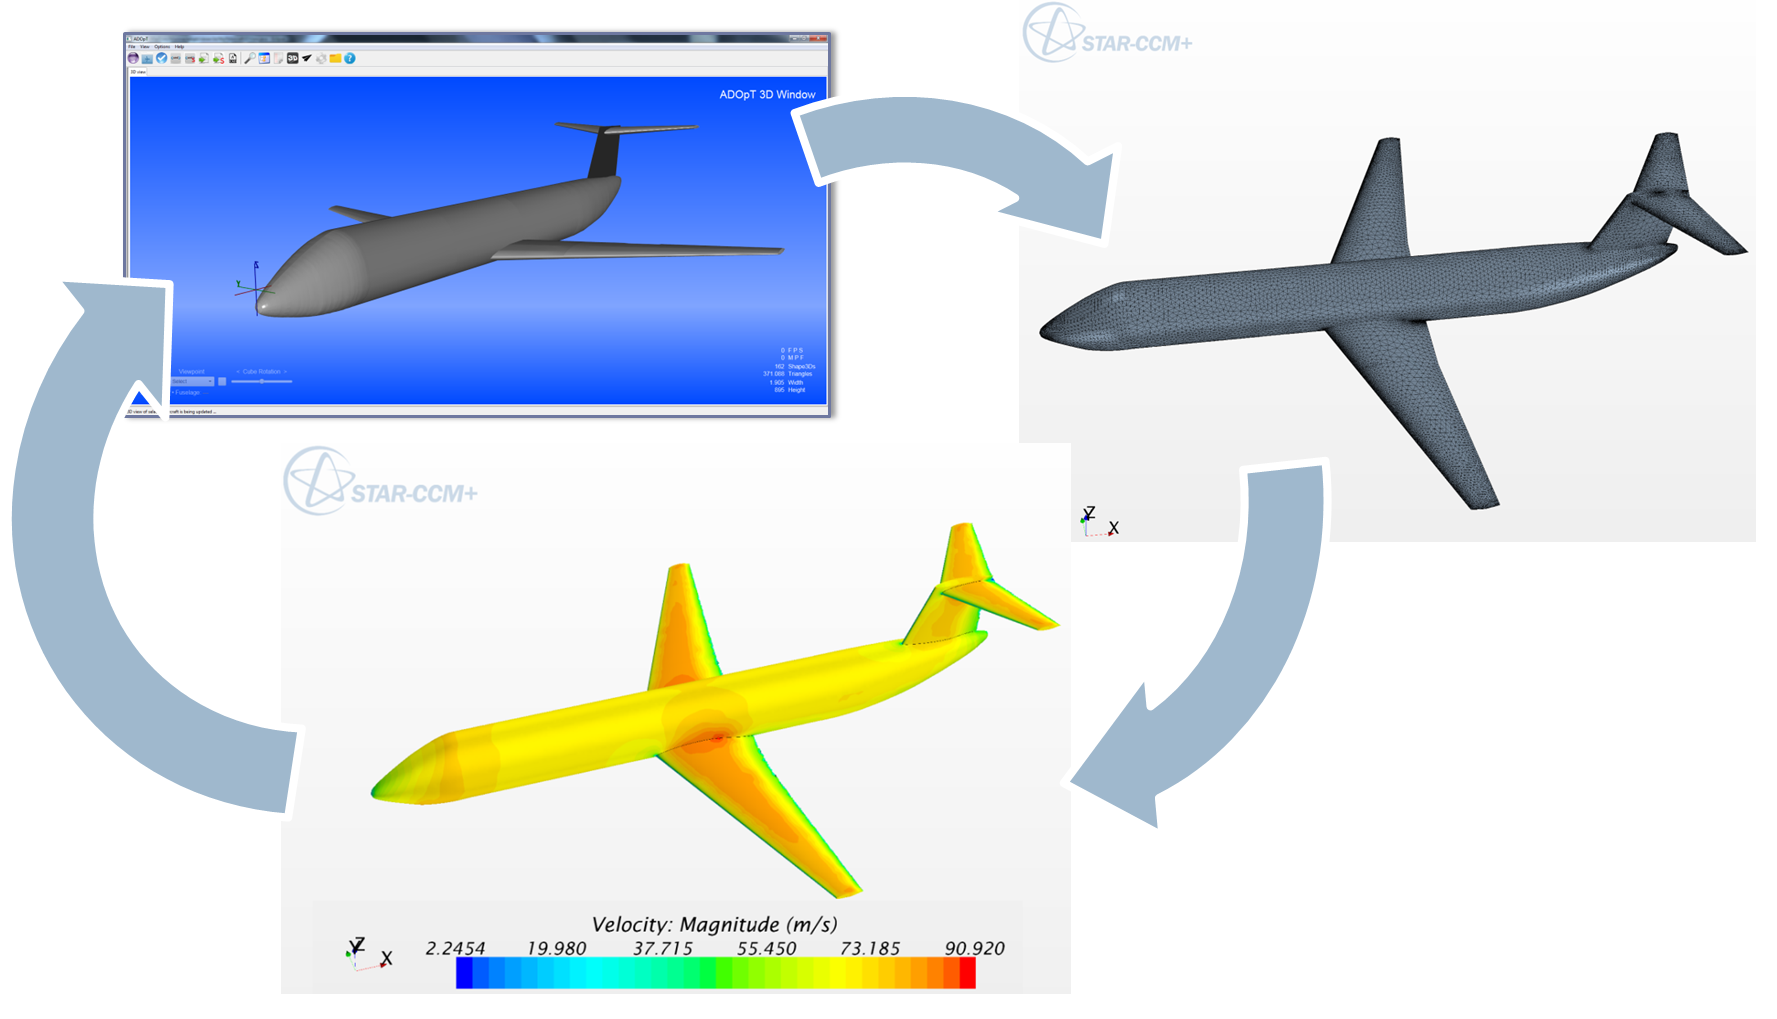
\includegraphics[width=12.9 cm]{Immagini/interface}
		\caption{Interface with external CFD tools.}
		\label{fig:badTail}
	\end{figure}
	
\section{In Development}

JPAD library is currently being developed in order to achieve a complete analysis of an aircraft and its optimization. The development is actually moving on a complete reorganization of the input file, and the implementation of other methods of analysis. Anyway, to date, it was reached an advanced level of implemented methods and a full functionality of some modules.

\subsection{Input File}

In order to obtain an useful and intuitive input structure a new data arrangement is in development. The JPAD input files are actually in XML data format. This extension will not change, but the purpose of the new structure is to allow the user to easily manage the input data in order to execute the desired analyzes.\\
The structure is inspired by that proposed by SUAVE. SUAVE is an open source suite constructed as a modular set of analysis tools written in Python and it is currently being developed in the Aerospace Design Lab at Stanford University. \cite{suave}
%This tool is based on a three input data structure as in the following figures.

\begin{figure}[H]
\centering
	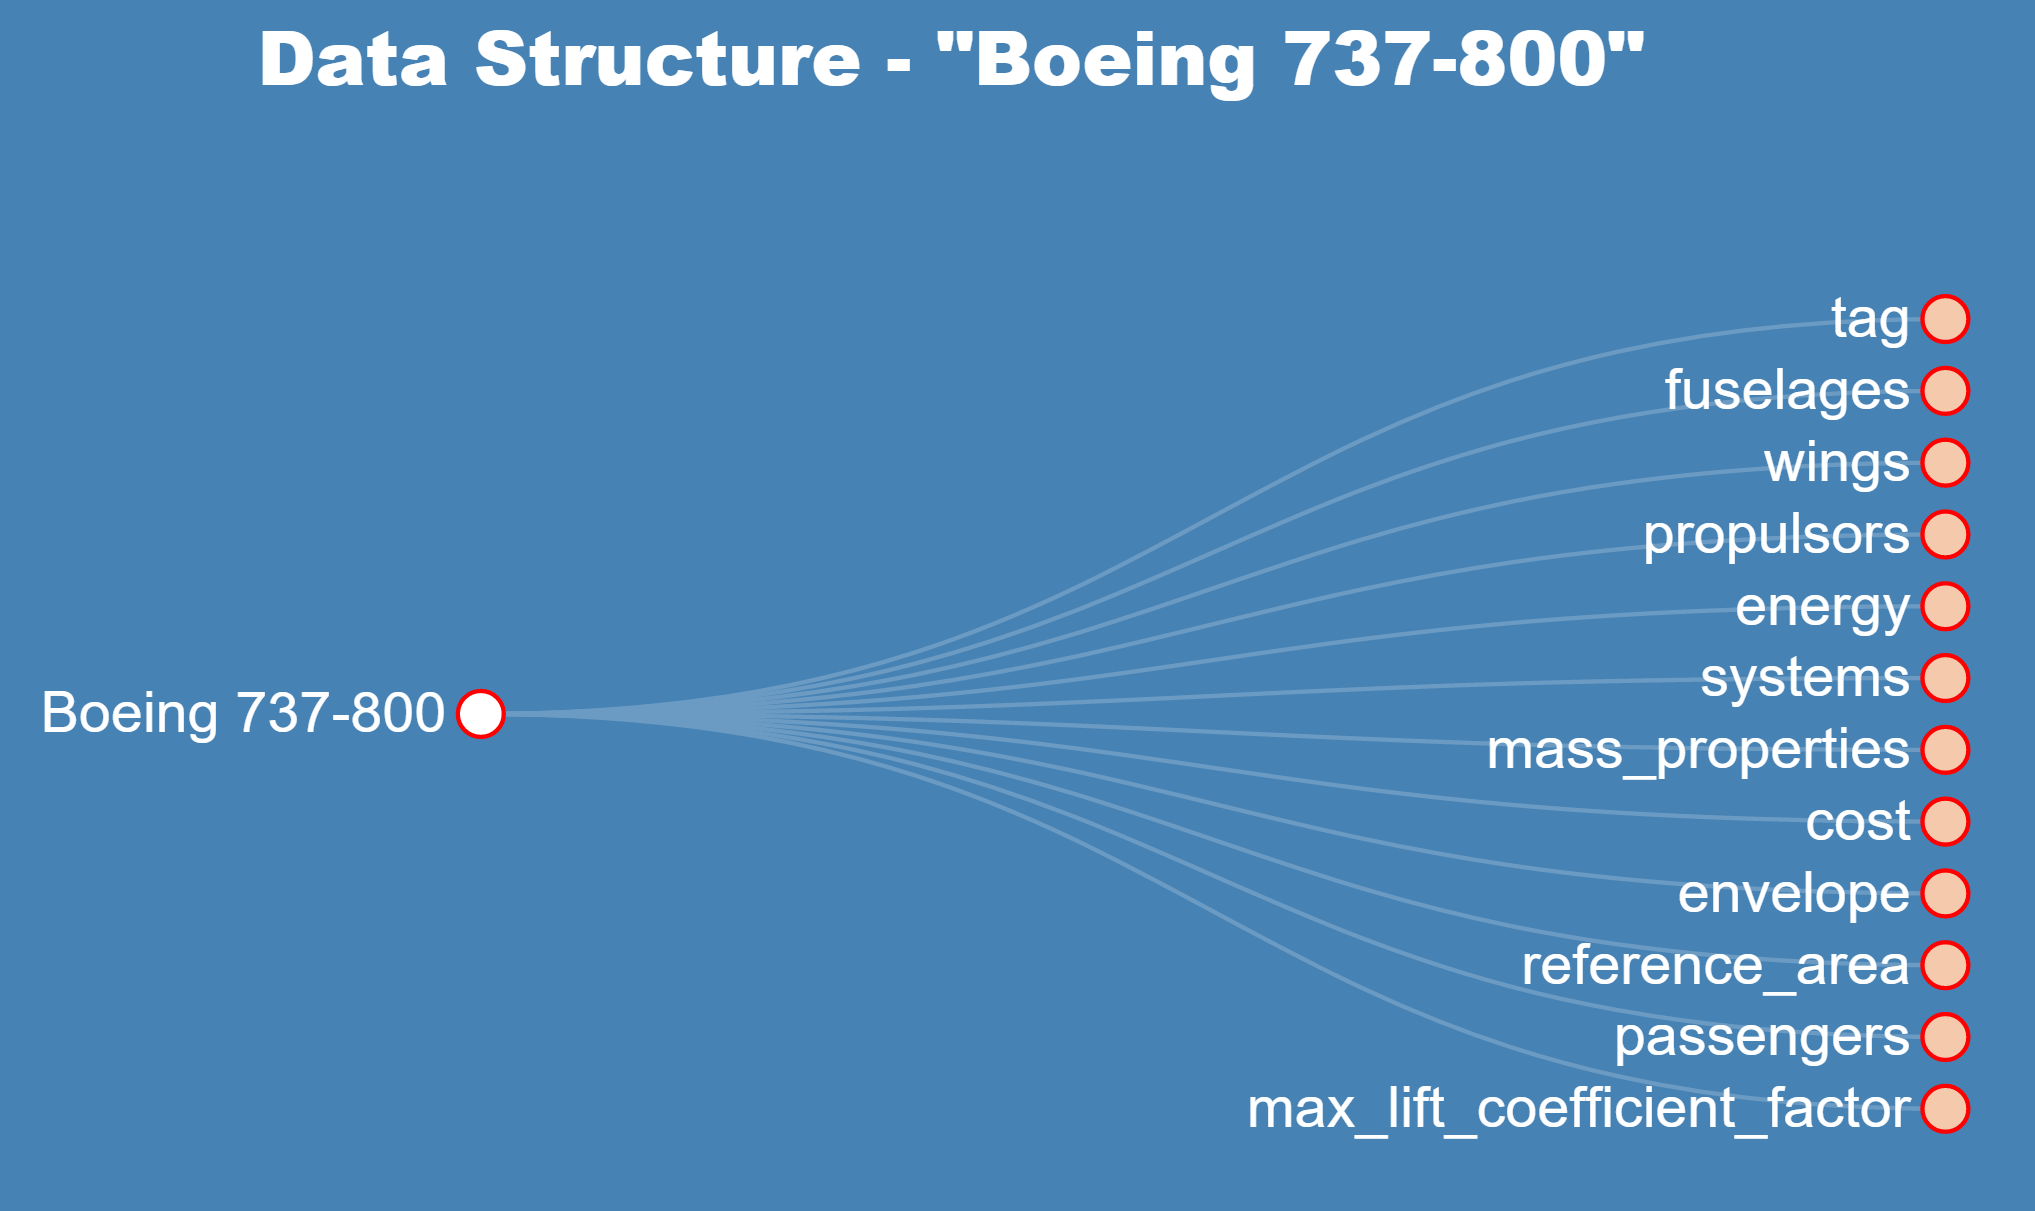
\includegraphics[width=11cm]{Immagini/suave/flowchartBoeing1}
	\caption{Data Structure used by SUAVE.}
	\label{fig:suave1}
\end{figure}

%
%\begin{figure}[H]
%	\centering
%	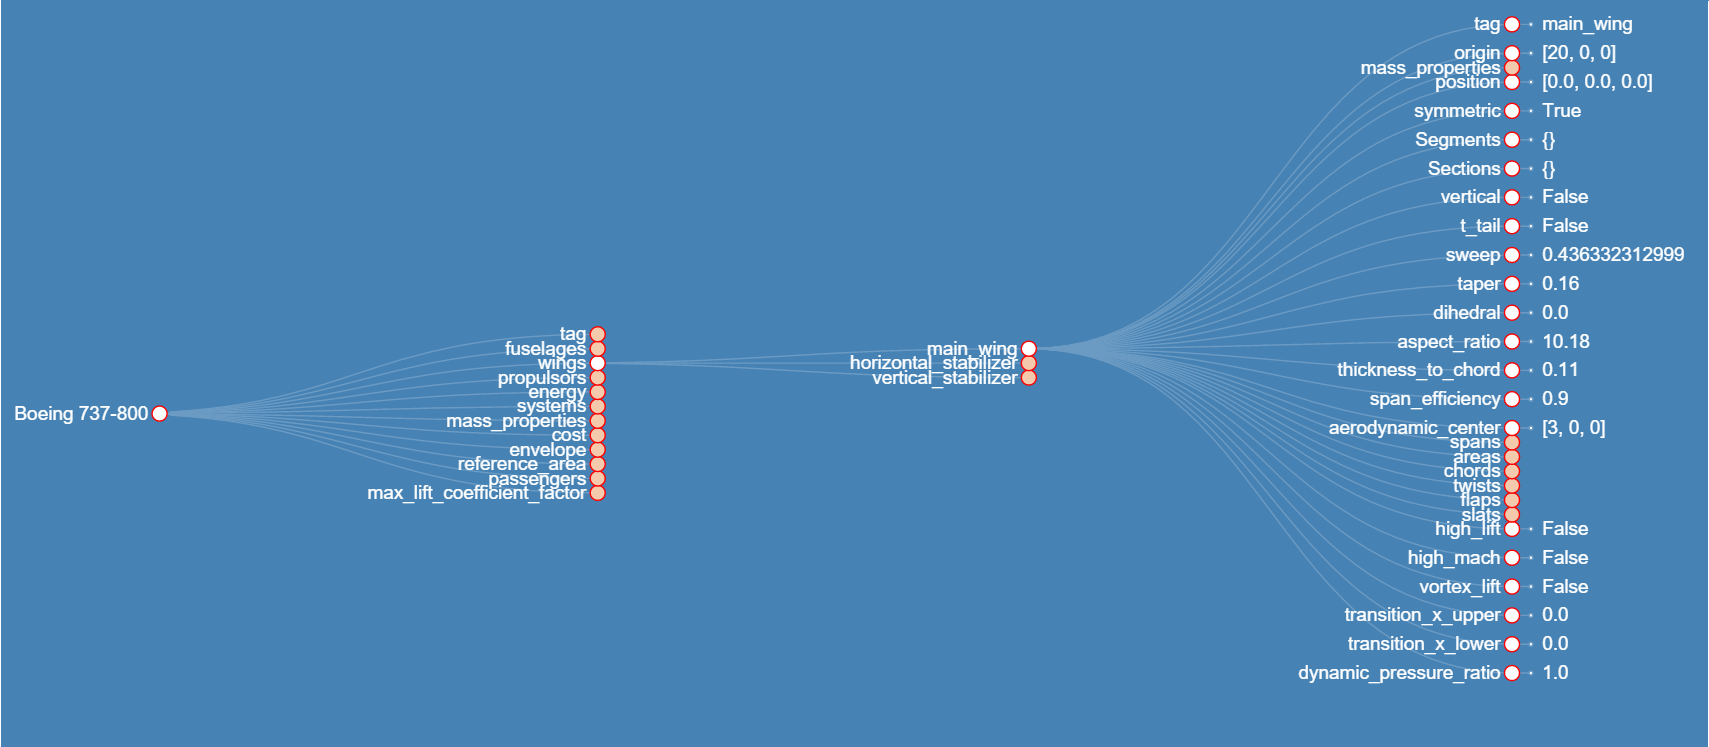
\includegraphics[width=12 cm]{Immagini/suave/flowchartBoeing2}
%	\caption{Data Structure used by SUAVE.}
%	\label{fig:suave2}
%\end{figure}



\begin{figure}[H]
\centering
	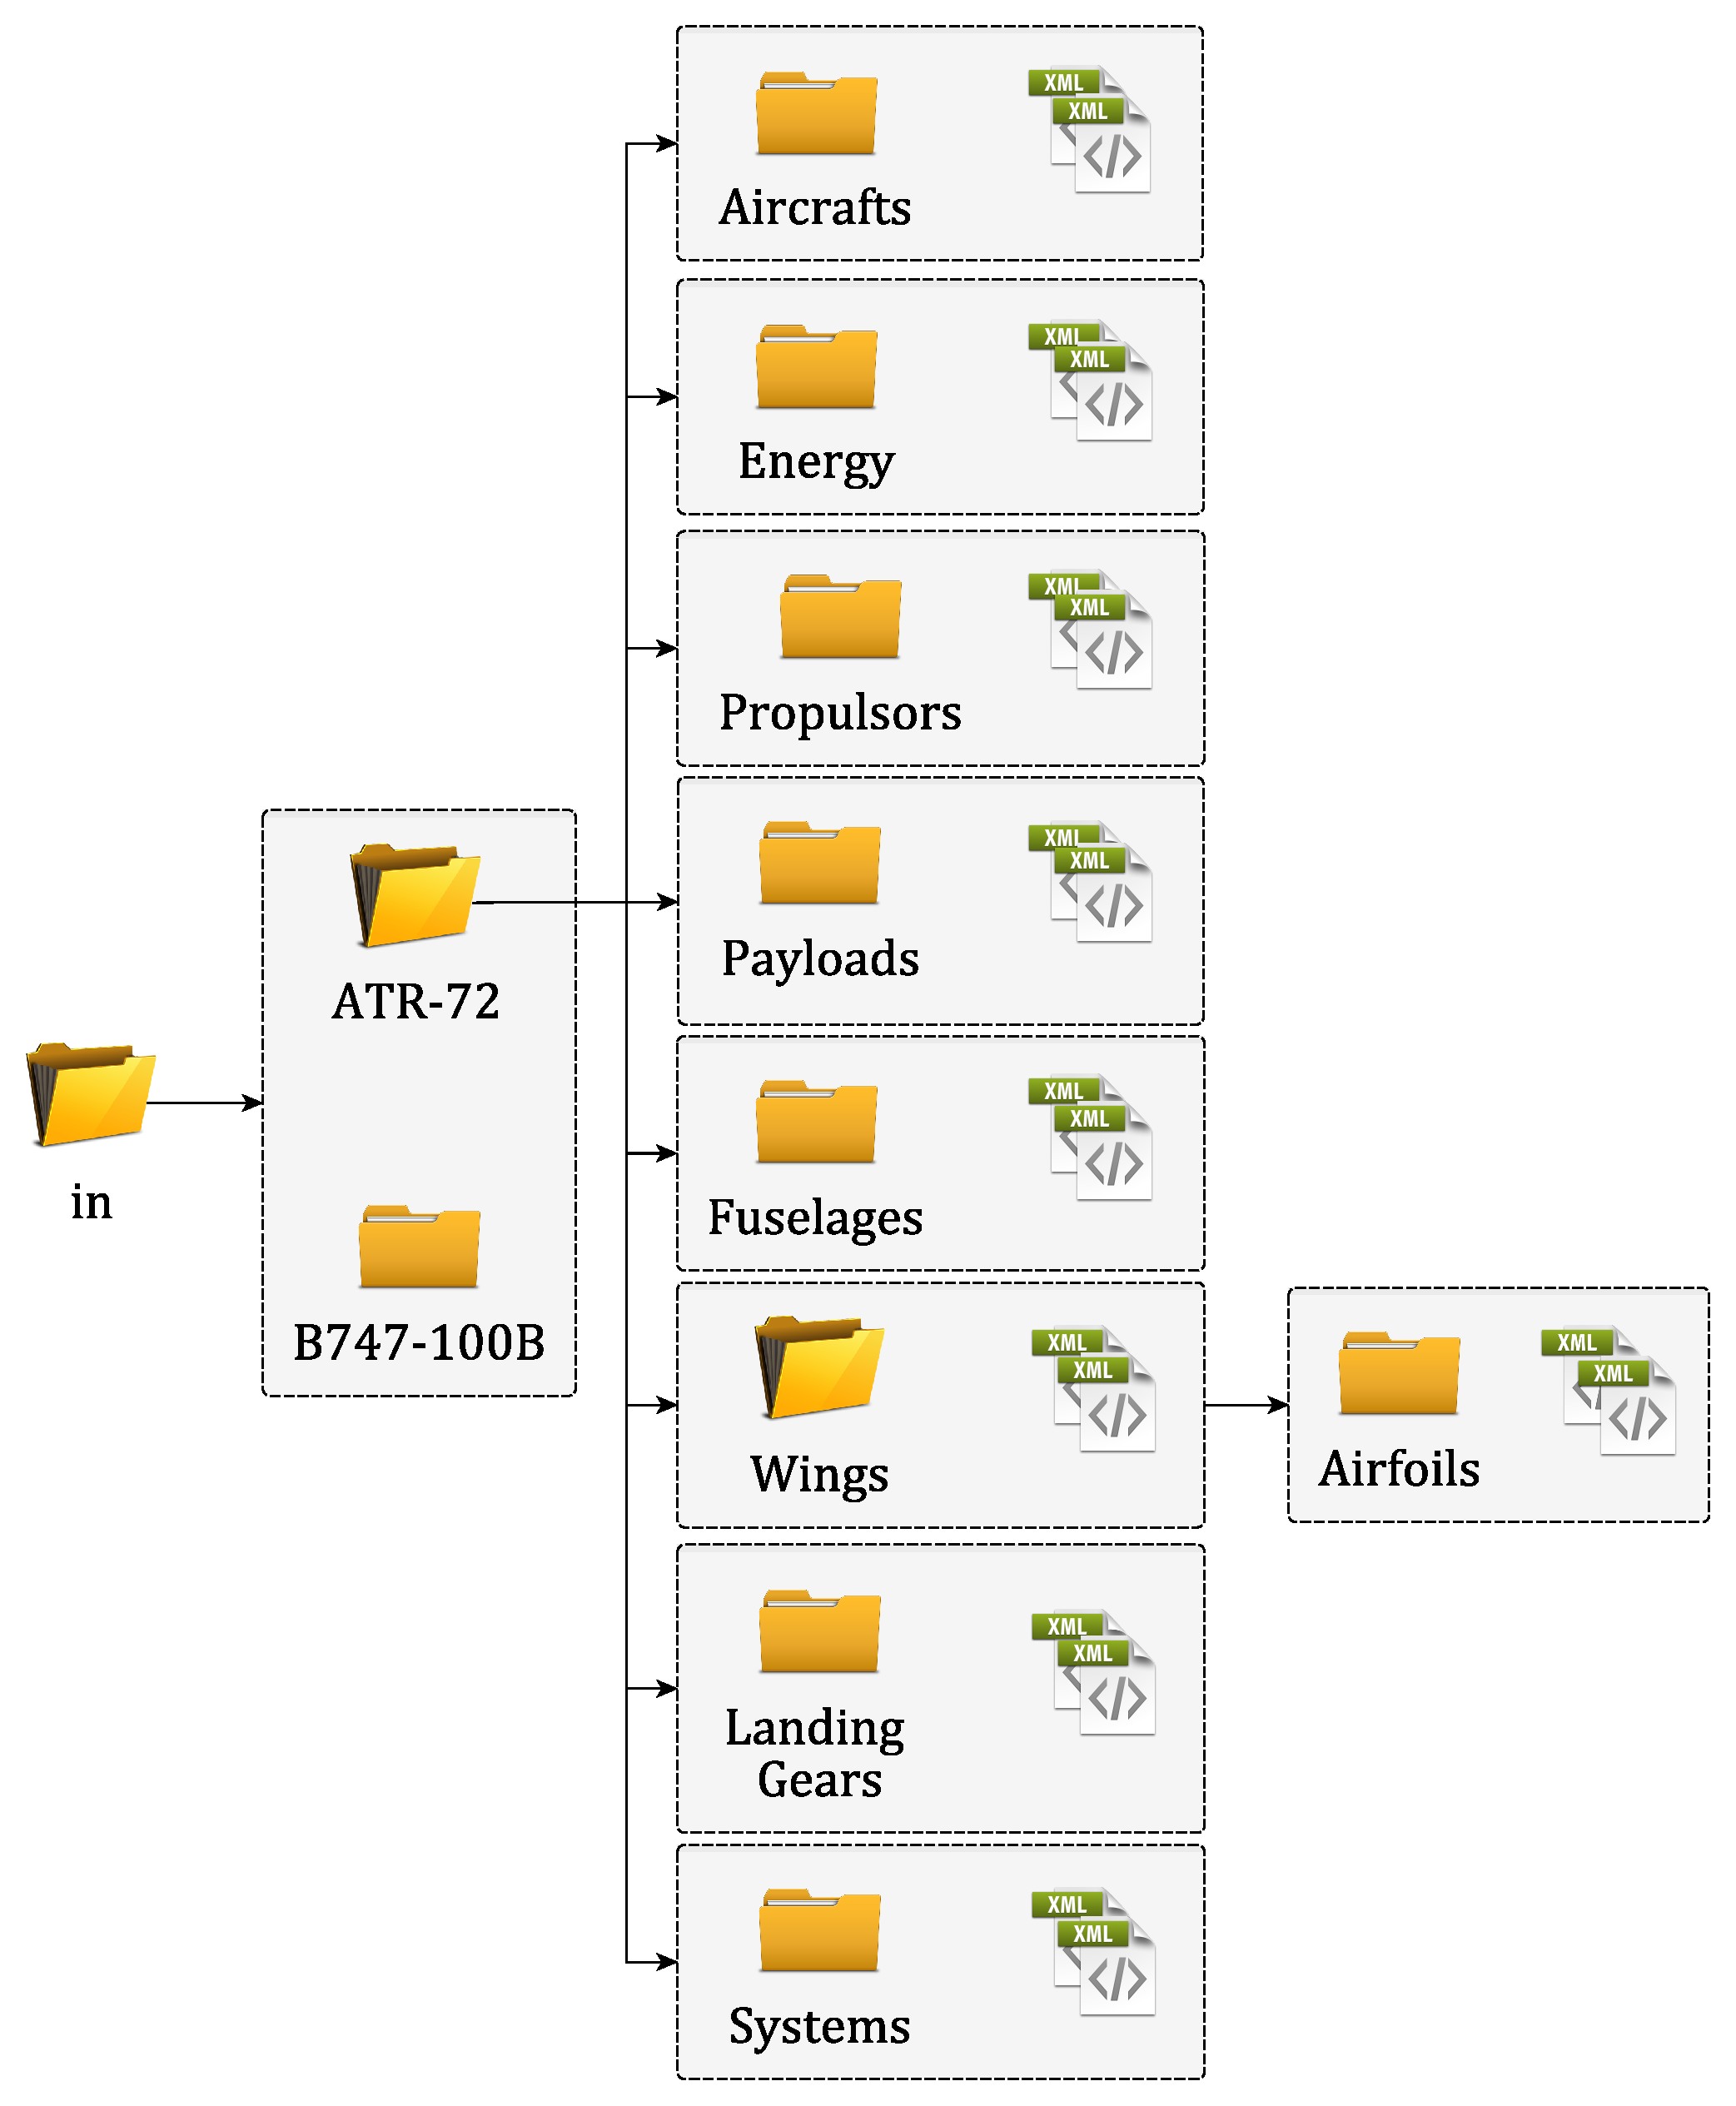
\includegraphics[width=11 cm]{Immagini/suave/Folder_Tree}
		\caption{Folder Structure in development.}
		\label{fig:suave3}
\end{figure}

The fundamental criteria on which the construction is based are expressed following.\\
In the input file folder, there are many sub-folder for different aircraft. In each of these there are several folders for component in which may be more XML file that corresponding to a different configuration. In fact, there is an XML file for each configuration of each aircraft component ( fuselage, lifting surfaces etc. ).In this way it's possible to choose different configuration for the same aircraft simply changing one or more XML input file.\\
 For the analysis the useful data will be explained in a user guide. User could make a complete analysis on a new aircraft, simply defining the required data and organize them in separated xml file. \\
 The main XML file is ``aircraft.xml'' which calls the other XML of the aircraft components. A typical file structure is in the following listings.
 
\begin{lstlisting}[frame=rbl,style=MyxmlStyle, caption={{\footnotesize XML input file for an aircraft.}},label= [style=\bfseries]{Listing}]
<?xml version="1.0" encoding="utf-8"?>
<jpad_config>
    <aircraft>
        <wings>
            <wing type="WING" file="wing.xml">
                <position>
                    <x unit="m">12.0</x>
                    <y unit="m"> 0.0</y>
                    <z unit="m"> 2.0</z>
                </position>
                <rigging_angle unit="deg">2.0</rigging_angle>
            </wing>
            <wing type="HTAIL" file="htail.xml">
                <position>
                    <x unit="m">30.0</x>
                    <y unit="m"> 0.0</y>
                    <z unit="m"> 4.0</z>
                </position>
                <rigging_angle unit="deg">0.0</rigging_angle>
            </wing>
            <wing type="VTAIL" file="vtail.xml">
                <position>
                    <x unit="m">30.0</x>
                    <y unit="m"> 0.0</y>
                    <z unit="m"> 5.0</z>
                </position>
                <rigging_angle unit="deg">0.0</rigging_angle>
            </wing>
        </wings>
        <fuselages>
            <fuselage file="fuselage.xml">
                <position>
                    <x unit="m">0.0</x>
                    <y unit="m">0.0</y>
                    <z unit="m">0.0</z>
                </position>
            </fuselage>
        </fuselages>
        <propulsors>
            <propulsor file="propulsor.xml">
                <position>
                    <x unit="m">12.0</x>
                    <y unit="m"> 5.0</y>
                    <z unit="m"> 0.0</z>
                </position>
                <tilting_angle unit="deg">2.0</tilting_angle>
                <yawing_angle unit="deg">0.0</yawing_angle>
            </propulsor>
            <propulsor file="propulsor.xml">
                <position>
                    <x unit="m">12.0</x>
                    <y unit="m">-5.0</y>
                    <z unit="m"> 0.0</z>
                </position>
                <tilting_angle unit="deg">2.0</tilting_angle>
                <yawing_angle unit="deg">0.0</yawing_angle>
            </propulsor>
        </propulsors>
    </aircraft>
</jpad_config>
\end{lstlisting}

\begin{lstlisting}[frame=rbl,style=MyxmlStyle, caption={{\footnotesize XML input file for an aircraft.}},label= [style=\bfseries]{Listing}]
<?xml version="1.0" encoding="utf-8"?>
<jpad_config>
    <wing mirrored="TRUE">
        <panels>
            <panel id="Inner panel">
                <semispan unit="m">4.0</semispan>
                <dihedral unit="deg">1.5</dihedral>
                <inner_section>
                    <airfoil file="naca63209.xml"/>
                    <geometric_twist unit="deg">0.0</geometric_twist>
                </inner_section>
                <outer_section>
                    <airfoil file="naca63209.xml"/>
                    <geometric_twist unit="deg">0.0</geometric_twist>
                </outer_section>
            </panel>
            <panel id="Outer panel" linked_to="Inner panel">
                <semispan unit="m">7.0</semispan>
                <dihedral unit="deg">3.5</dihedral>
                <outer_section>
                    <airfoil file="naca63209.xml"/>
                    <geometric_twist unit="deg">-2.5</geometric_twist>
                </outer_section>
            </panel>
        </panels>
        <symmetric_flaps>
            <symmetric_flap id="Inner flap" type="SINGLE_SLOTTED">
                <inner_station_spanwise_position type="PERCENT_SEMISPAN" ref_to="FULL_SEMISPAN">
                    <value>0.15<value/>
                </inner_station_spanwise_position>
                <outer_station_spanwise_position type="PERCENT_SEMISPAN" ref_to="FULL_SEMISPAN">
                    <value>0.45<value/>
                </outer_station_spanwise_position>
                <percent_chord value="40"/>
                <angle_range unit="deg">[0.0,40.0]</angle_range>
            </symmetric_flap>
        </symmetric_flaps>
        <slats>
            <slat linked_to="Inner flap" type="SINGLE">
                <percent_chord value="10"/>
                <angle_range unit="deg">[0.0,10.0]</angle_range>
            </slat>
        </slats>
        <asymmetric_flaps>
            <asymmetric_flap id="Aileron" type="PLAIN">
                <inner_station_spanwise_position type="PERCENT_SEMISPAN" ref_to="FULL_SEMISPAN">
                    <value>0.75<value/>
                </inner_station_spanwise_position>
                <outer_station_spanwise_position type="PERCENT_SEMISPAN" ref_to="FULL_SEMISPAN">
                    <value>0.97<value/>
                </outer_station_spanwise_position>
                <percent_chord value="20"/>
                <angle_range unit="deg">[-5.0,10.0]</angle_range>
                <differential_deflection_factor value="1.0"/>
            </asymmetric_flap>
        </asymmetric_flaps>
    </wing>
</jpad_config>
\end{lstlisting}

\subsection{Calculation modules}
Currently the software is able to esimate the aircraft weight breakdown, the center of gravity location, calculate some aerodynamic parameters and estimate the performance. All these types of estimates can be usually performed using several analysis methods, comparable and interchangeable. 
It is also provided a static longitudinal stability analysis, take-off performances and the generation of Payload Range chart.\\
Future targets for the software are the implementation of landing performances, ultimate the directional static stability % ... 


\subsection{Optimization Process}
It has always been the engineer’s dream to have all aspects of analysis done in a relatively short time period so that many different configurations can be examined and the best suitable product can be delivered on time. Although this may still be a dream, actual design turn-around time has become shorter due to the use of mathematical optimization techniques which have been
introduced into the design process.\cite{torenbeek2013advanced}
As all analysis modules inside the JPADCore package will be completed and tested, the final purpose of the code will be to allow users to define a certain numbers of macroscopical geometrical parameters, along with a given objective function, and to receive as output the best set of the previous parameters which suits the wanted objective.



\part{Development of Application}
\chapter{Introdution to Java}
\label{ch:java}
\markboth{Introdution to Java}{}


\begin{flushright}
	{\smaller
		\textit{Language is only the instrument of science, \\and words are but the signs of ideas.}\\
		-- Samuel Johnson}
\end{flushright}


\section{The java Language}
The term Java refers both to a programming language with the higher number of developers in the worldwide and to a technology that has several sub-technologies that have emerged in different fields of use of the software. Javawas developed by Sun Microsystems, a company that was incorporated in Oracle from a few years.
In 1996, James Gosling, Bill Joy, and Guy Steele wrote for the First Edition of The Java Language Specification:
``{\itshape We believe that the Java programming language is a mature language, ready for widespread use. Nevertheless, we expect some evolution of the language in the years to come. We intend to manage this evolution in a way that is completely compatible with existing applications.}''\\
This programming language is a general-purpose, concurrent, classbased, object-oriented language. It is designed to be simple enough that many programmers can achieve fluency in the language.\cite{javaoracle}
One design goal of Java is portability, which means that programs written for the Java platform must run similarly on any combination of hardware and operating system with adequate runtime support. This is achieved by compiling the Java language code to an intermediate representation called Java bytecode, instead of directly to architecture-specific machine code. Java bytecode instructions are analogous to machine code, but they are intended to be executed by a virtual machine (VM) written specifically for the host hardware. End users commonly use a Java Runtime Environment (JRE) installed on their own machine for standalone Java applications, or in a web browser for Java applets.\cite{wiki:java}
Standard libraries provide a generic way to access host-specific features such as graphics, threading, and networking.\\
There were five primary goals in the creation of the Java language:\cite{java}
\begin{enumerate}
\item It must be ``simple, object-oriented, and familiar''.
\item It must be ``robust and secure''.
\item It must be ``architecture-neutral and portable''.
\item It must execute with ``high performance''.
\item It must be ``interpreted, threaded, and dynamic''.
\end{enumerate}
Java SE 8 represents the single largest evolution of the Java language in its history. A relatively small number of features - lambda expressions, method references, and functional interfaces - combine to offer a programming model that fuses the objectoriented
and functional styles. Under the leadership of Brian Goetz, this fusion has been accomplished in a way that encourages best practices - immutability, statelessness, compositionality - while preserving ``the feel of Java'' - readability, simplicity, universality.\\
Actually Java is the most used programming language according to TIOBE. The TIOBE Programming Community index is an indicator of the popularity of programming languages. The ratings are based on the number of skilled engineers world-wide, courses and third party vendors.


\section{Java choice}

The software presented in this thesis work is completely written in Java. The choice of the programming language was driven by several considerations. These include the following:

\begin{itemize}
\item the language should be widely supported; this to avoid the case of many valid aircraft design applications and libraries that became obsolete due to the aging of the programming language used to build them;
\item the language should promote the use of open source libraries, especially for I/O tasks and for complex mathematical operations;
\item the language and the companion \gls{acr:ide} should provide a widely supported \gls{GUI} framework and a \gls{GUI} visual builder;
\item  the language should support and promote modularity.
\end{itemize}
The Java programming language meets all these requirements: it is backed by Oracle and by a huge community of developers so it is continuously updated. Also, advanced and free \gls{acr:ide}s (such as Eclipse) allow programmers to streamline and simplify the development process. In particular, the Eclipse \gls{acr:ide} and the SWT/JFace libraries have been chosen to develop \gls{acr:Jpad} and its \gls{GUI}.
Being Java a pure object oriented programming language, it greatly encourages and simplifies modularization. Each module (package) can be programmed quite independently so that it is relatively easy to divide the work among several programmers. This is essential since the amount of classes and calculations needed to abstract, manage and analyze the entire aircraft is very large (presently the whole project counts more than 56000 lines of code). For such a reason the establishment of common practices and the adherence to fundamental principle of software development (Don’t Repeat Yourself, Separation of Concerns, Agile software development) are equally important.
An important design requirement of \gls{acr:Adopt} is related to its interoperability with other engineering analysis tools. In fact, the application can be easily integrated into a comprehensive aircraft optimization cycle. This is made possible because \gls{acr:Adopt} can be launched both in \gls{GUI} and command line mode. Much care has been given to input/output and configuration files to increase the possible uses of the software.\cite{adoptunina}

\begin{figure}[H]
\centering
{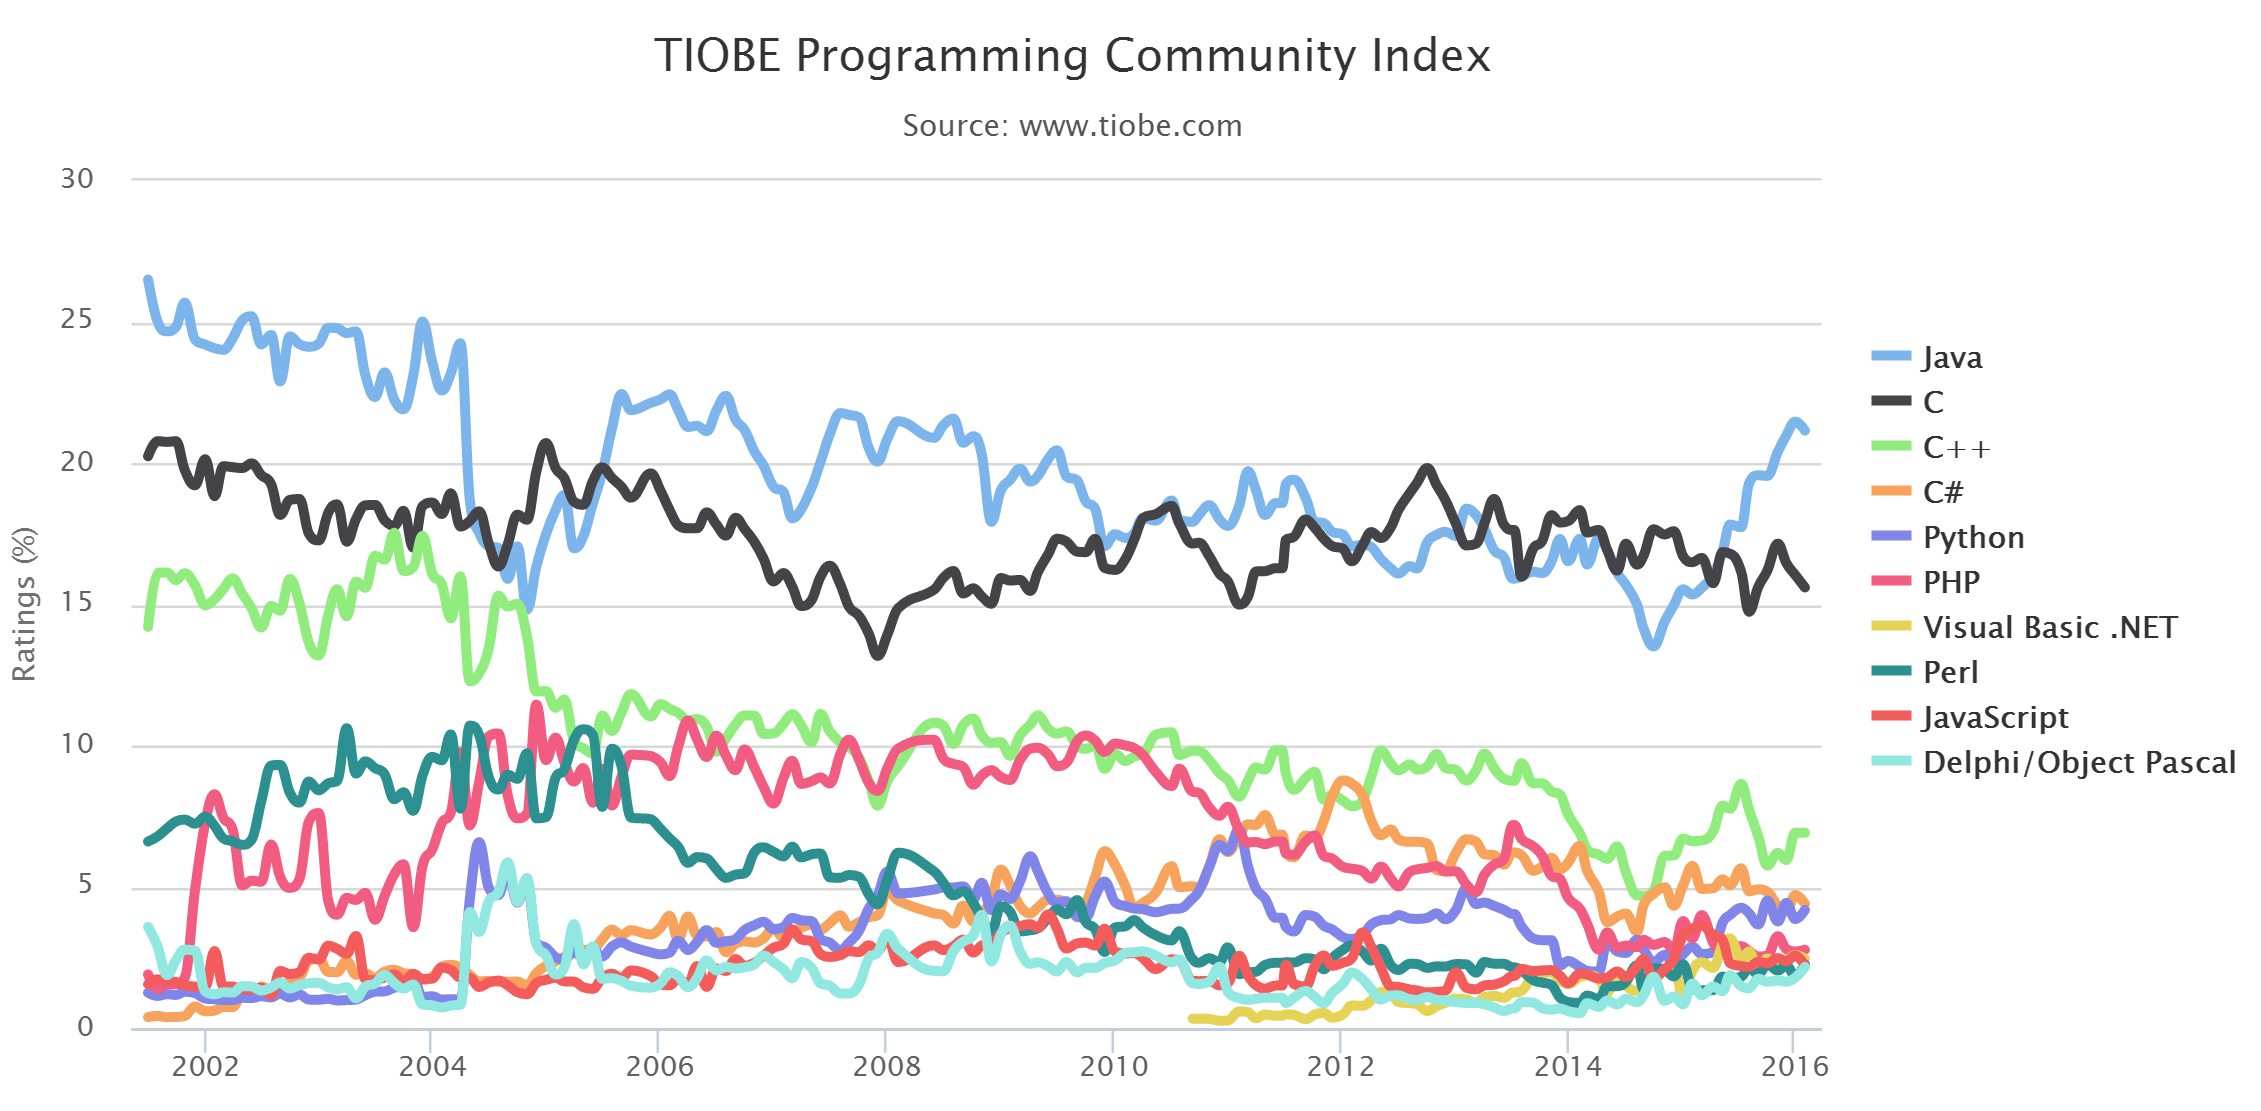
\includegraphics[height=7.6cm ]{Immagini/trend.png}} 
\caption{Programming Language popularity trade.}
\label{fig:hl}
\end{figure}







\chapter{Work Object}%
\label{ch:workobject}
\markboth{Work Object}{}
\begin{flushright}
	{\smaller
		\textit{If the facts don`t fit the theory,\\change the facts. }\\
		-- Albert Einstein}
\end{flushright}
\section {Introduction}
In JPAD it is possible to read an .XML file as input or generate an object whose data are written in the code. Both in the first and in the second case all needed variables are initialized with data relating the chosen aircraft. The difference between these two methods is that using an .XML file, user can define its own aircraft having a clear view about the needed data useful for the analysis.\\
Contrariwise in order to perform a test of program functionality, to use a default aircraft is the most simple way to generate a work object.

\section {Input data from .XML file}
%\subsection{XML File Format}
XML is a file extension for an {\itshape Extensible Markup Language (XML)} file format which is a markup language that defines a set of rules for encoding documents in a format which is both human-readable and machine-readable. Although the design of XML focuses on documents, it is widely used for the representation of arbitrary data structures such as those used in web services. It is defined ``Markup Language'' due to the use of tags that describes the content. XML is considered extensible because the markup symbols are unlimited and self-defining. So it is possible to use a personal tag for each data. In this way to read an .XML file results relatively simple.\cite{wiki:xml}\\
The key concepts of an .XML File Format are the followings:
\begin{itemize}
\item markup symbol (tag)
\item attribute
\item tree structure
\end{itemize}

As mentioned, each part of the test is contained between an opening {\bfseries markup symbol} and an end markup symbol that expressed the meaning of the text.\\

\begin{figure}[H]
\centering
{
\includegraphics[height=0.31cm]{Immagini/xml1.jpg}} 
\caption{Use of markup symbols in XML language.}
\end{figure}

In addition to tag name, the markup symbols may contain also some {\bfseries attributes} that introduce more informations such as the unit of measure.\\

\begin{figure}[H]
\centering
{
\includegraphics[height=0.4cm]{Immagini/xml2.jpg}} 
\caption{Use of attributes in XML language.}
\end{figure}

An .XML file has a tree structure in which external knots that branch into internal knots.
%\noindent \\
%
%\begin{figure}[H]
%\centering
%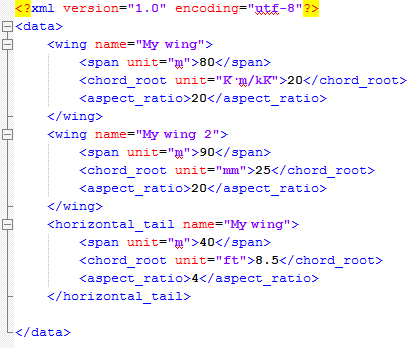
\includegraphics[height=6cm]{Immagini/xml5.png}\hfil
%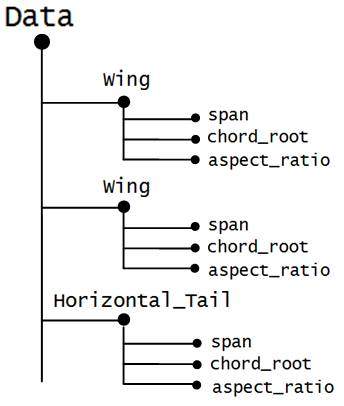
\includegraphics[height=6cm]{Immagini/xml3.jpg}
%\caption{Tree structure of an .XML file.}
%\end{figure}

%\subsection{Data Managment from XML file.}
In order to read an XML file it is necessary, first of all, to give the file path. The class \texttt{JPADXmlReader} opens the file and  the methods of the class \texttt{MyXMLReaderUtils} read the useful data from the XML having the tag path as input. It is possible to read data as \texttt{Amount}, namely with units of measurement or as \texttt{double}. The unit of measurement is written in the attributes of data in XML file.\\ 

Likewise it is possible to write output data on XML file using \texttt{JPADDataWriter} class. First of all it is necessary to define and build the xml tree structure. After each variable is associated with a name that is the markup symbol of the XML file.

%possibili sviluppi futuri

\section {Default Aircraft}
At the moment it is possible to define two different aircrafts in order to test the functionality of the application: {\bfseries ATR-72}  and {\bfseries B747-100B}. \\ \\

The {\bfseries ATR 72} is a twin-engine turboprop made by the French-Italian aircraft manufacturer ATR entered service in 1989.  It was developed as a variant of the ATR 42  with a 4.5 m stretched fuselage.  The ATR 72 was developed from the ATR 42 in order to increase the seating capacity (48 to 66 in standard configuration) by stretching the fuselage, increasing the wingspan, adding more powerful engines, and increasing fuel capacity by approximately 10 percent. It has been typically employed as a regional airliner, although other roles have been performed by the type such as corporate transport, cargo aircraft and maritime patrol aircraft. \cite{wiki:atr}


\begin{figure}[H]
\centering
{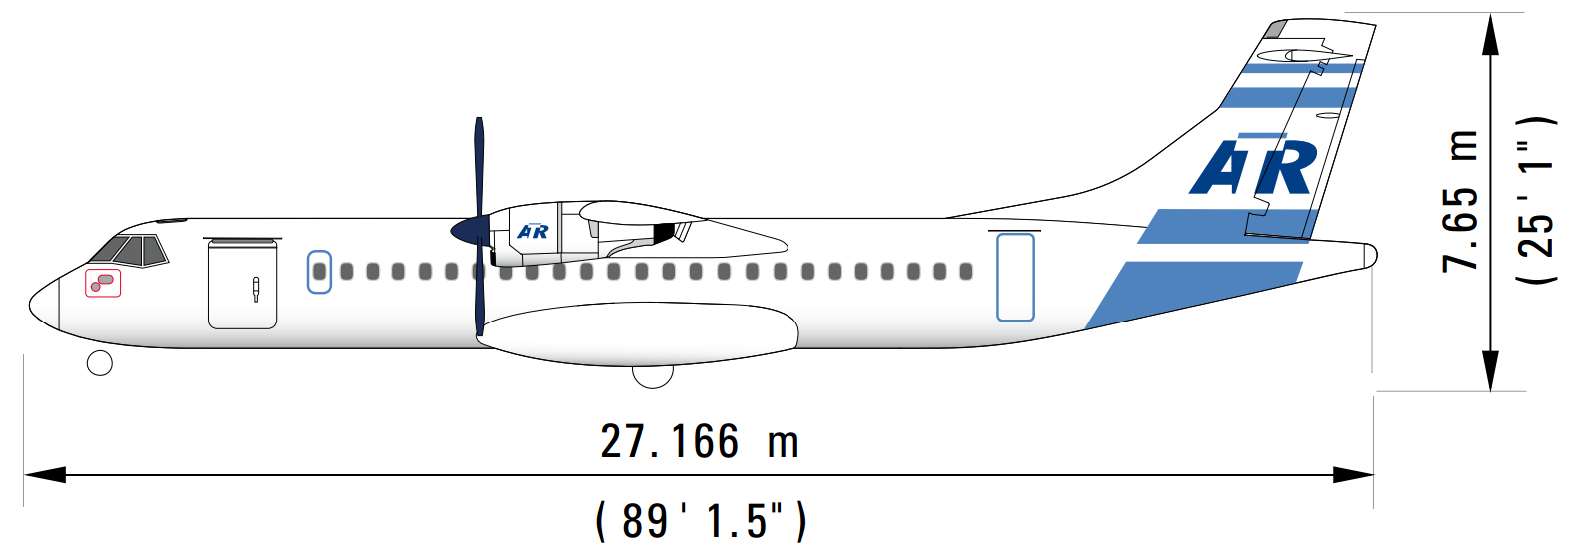
\includegraphics[height=4cm]{Immagini/atr72mod.jpg}} 
\caption{ATR 72. Side view.}
\end{figure}


The {\bfseries Boeing 747-100B} is a four-engined long-range widebody commercial jet airliner and cargo aircraft  produced by the American manufacturer Boeing Commercial Airplanes. It has a capacity of maximum 480 passengers in a partial double deck configuration. The Boeing 747 is also known as Jumbo Jet. The basic B747-100 entered service with Pan American On January 15, 1970.\\
One of the reasons to create the 747 was reductions in airfares with a consequent increase of passenger traffic\cite{wiki:boeing}. The original version of the 747 had two and a half times greater capacity than the Boeing 707, one of the common large commercial aircraft of the 1960s and it was the largest passenger carrier from 1970 until the introduction of Airbus A380.
The Boeing 747 has two aisles and four wing-mounted engines. The upper deck is its distinctive "hump" along the forward part of the aircraft. It provides space for a lounge or extra seating. The raised cockpit allows front loading of cargo on freight variants. \\
The 747-100B model was developed from the 747-100SR. This configuration has a typical 452 passengers and unlike the original 747-100, the 747-100B was offered with Pratt \& Whitney JT9D-7A, General Electric CF6-50, or Rolls-Royce RB211-524 turbofan engines.

\begin{figure}[H]
\centering
{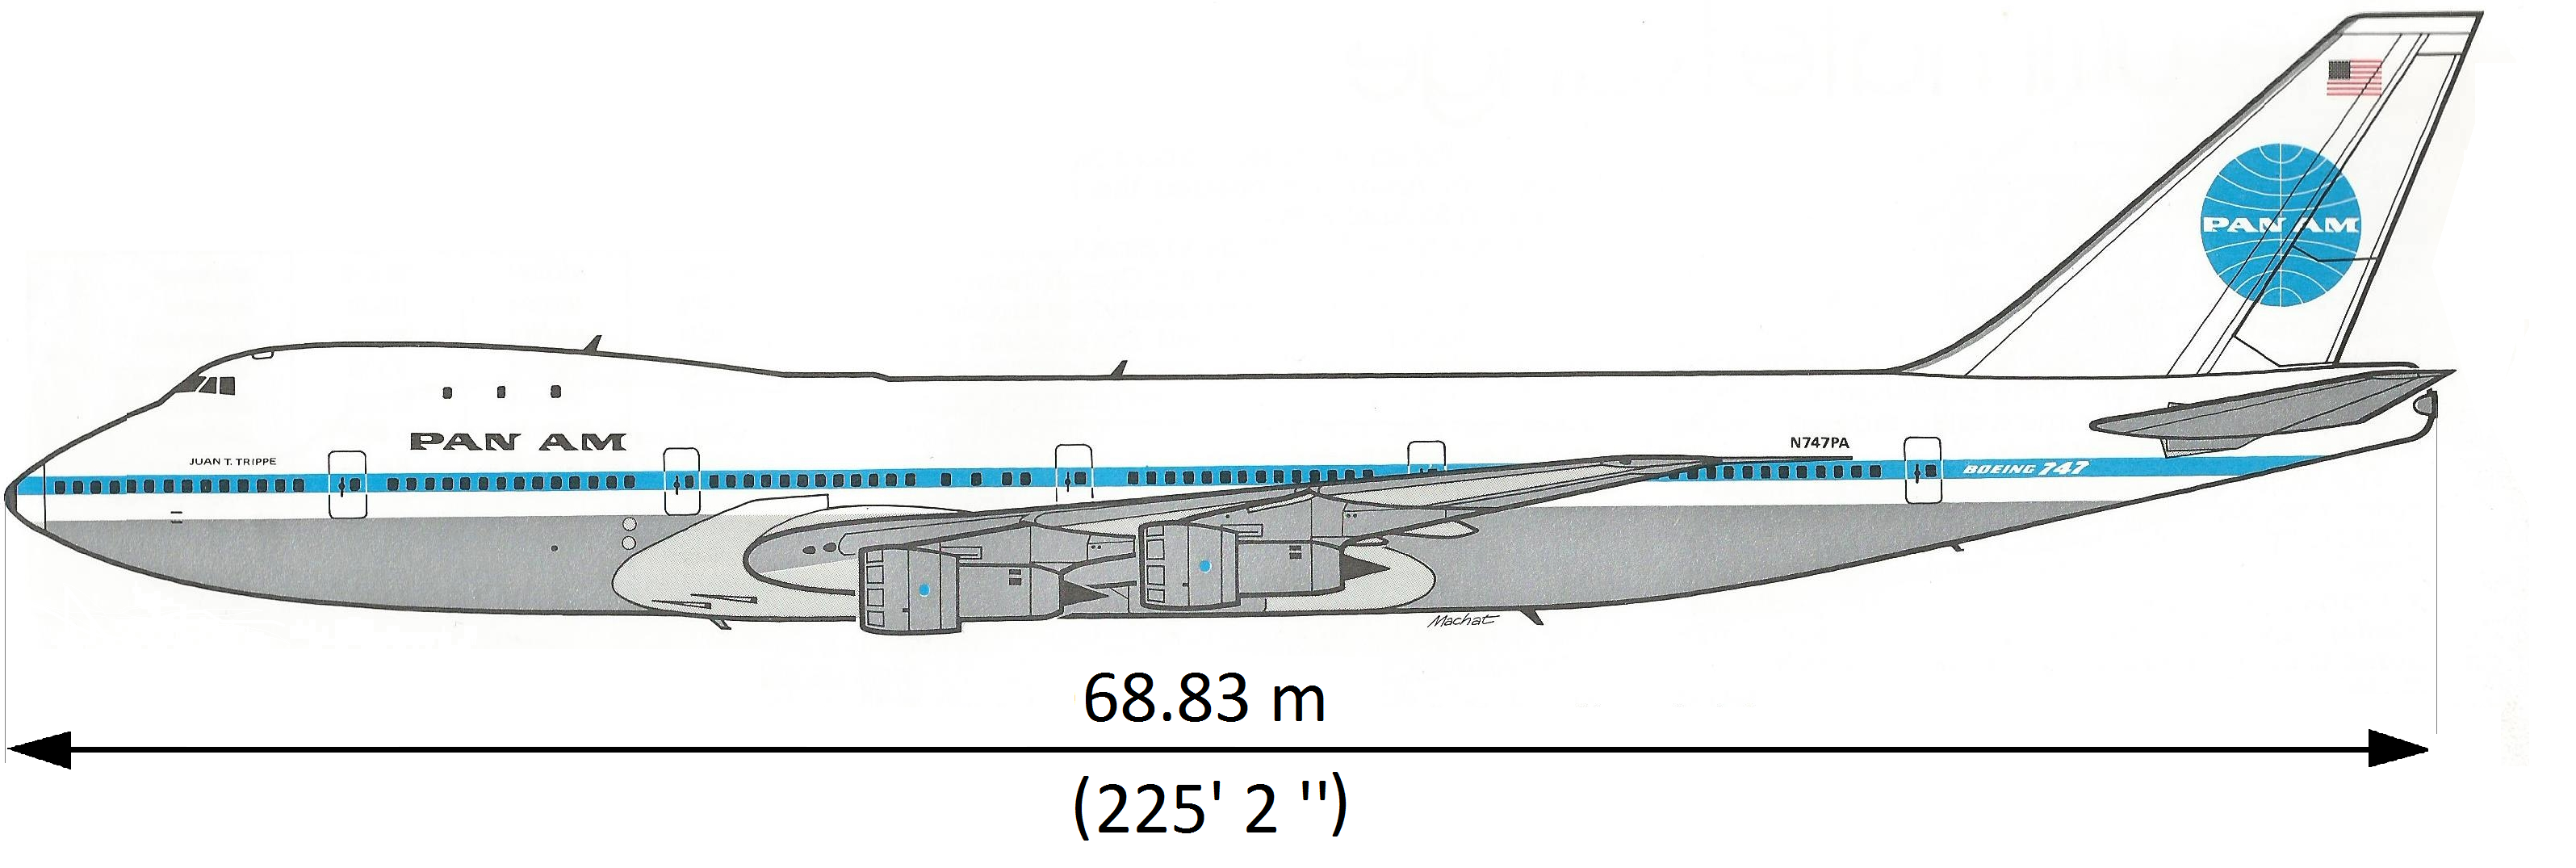
\includegraphics[height=4cm]{Immagini/boeing.jpg}} 
\caption{Boeing 747-100B. Side view.}
\end{figure}

\subsection {How is made a default Aircraft}
In order to define a Default Aircraft in a test class, and use it to check the functionalities of the application, it is necessary to follow some steps. First of all it is necessary to initialize the working directory tree using the method \texttt{initWorkingDirectoryTree} of \texttt{MyConfiguration} class located in \texttt{JPADConfigs} package that initializes the working directory tree and fills the map of folders. 
This step is required in order to create the following default folders that are necessary for the right behavior of the code:

\begin{itemize}
\item Database directory
\item Input directory
\item Output directory
\end{itemize}

Using  \texttt{MyConfiguration} class is possible to point at a specific folder, like the input or output directory, with the static method  \texttt{getDir}. This is a crucial step that must be executed at the beginning of every test.
To set the working directory with the useful folders, is necessary to call the function \texttt{initWorkingDirectoryTree()} at the beginning of each test. The function creates all necessary folders. Morover the function has been overloaded and it can be even called with a variable number of arguments (\texttt{initWorkingDirectoryTree( String...str)}). These strings are the directory strings in \texttt{MyConfiguration} class.
The second step is the creation of an\texttt{Aircraft} object choosing between the ones grouped into a dedicated \texttt{Enum}, named \texttt{AircraftEnum}.
After it is possible to create an \texttt{Aircraft} using the method \texttt{createDefaultAircraft} from \texttt{Aircraft} class. This method defines a new Aircraft object and invokes another Aircraft's method that creates the components using default data. In the method \texttt{createDefaultAircraft} there is a calling to the builder of \texttt{Aircraft} class that initializes the objects of the classes that perform calculations. At this step all the components of the aircraft are created. It is possible also to define new airfoils for the aircraft or change some data from the existing. \\
Afterwards it is necessary to set the operating conditions such as the number of Mach of analysis or altitude. Each default aircraft has a set of default conditions but the user could change them.\\
In order to manage all the aircraft related analyses it is necessary to define an object of the class  \texttt{ACAnalysisManager}. Similarly to the aircraft, an analysis manager  exists also for the wing that is an object of the  \texttt{LSAerodynamicManager} class. \\
The next step is to define and assign the needed databases. This will be explained in detail in the next section. Finally it is possible to do analysis.

\noindent \\
\begin{lstlisting}[frame=rbl,caption={{\footnotesize Generation of default aircraft}},label= [style=\bfseries]{Listing}]
public static void main(String[] args) {

	// --------------------------------------------------------------
	// Define directory
	// --------------------------------------------------------------
	MyConfiguration.initWorkingDirectoryTree();


	// --------------------------------------------------------------
	// Generate default Aircraft
	// --------------------------------------------------------------
	Aircraft aircraft = Aircraft.createDefaultAircraft(AircraftEnum..B747_100B);
	LiftingSurface theWing = aircraft.get_wing();

	// Default operating conditions
	OperatingConditions theConditions = new OperatingConditions();		


	// --------------------------------------------------------------
	// Define an ACAnalysisManager Object
	// --------------------------------------------------------------
	ACAnalysisManager theAnalysis = new ACAnalysisManager(theConditions);
	theAnalysis.updateGeometry(aircraft);


	// --------------------------------------------------------------
	// Define an LSAerodynamicsManager Object
	// --------------------------------------------------------------
	LSAerodynamicsManager theLSAnalysis = new LSAerodynamicsManager ( 
			theConditions,
			theWing,
			aircraft
			);

		
	// --------------------------------------------------------------
	// Setup database(s)	
	// --------------------------------------------------------------
		
	theLSAnalysis.setDatabaseReaders(
			new Pair(DatabaseReaderEnum.AERODYNAMIC,
                          "Aerodynamic_Database_Ultimate.h5"),
			new Pair(DatabaseReaderEnum.HIGHLIFT,  
                          "HighLiftDatabase.h5")
			);

	
	// --------------------------------------------------------------
	// Do analysis
	// --------------------------------------------------------------
	theAnalysis.doAnalysis(aircraft, 
			AnalysisTypeEnum.AERODYNAMIC);
}
\end{lstlisting}

\begin{sidewaysfigure}

\centering
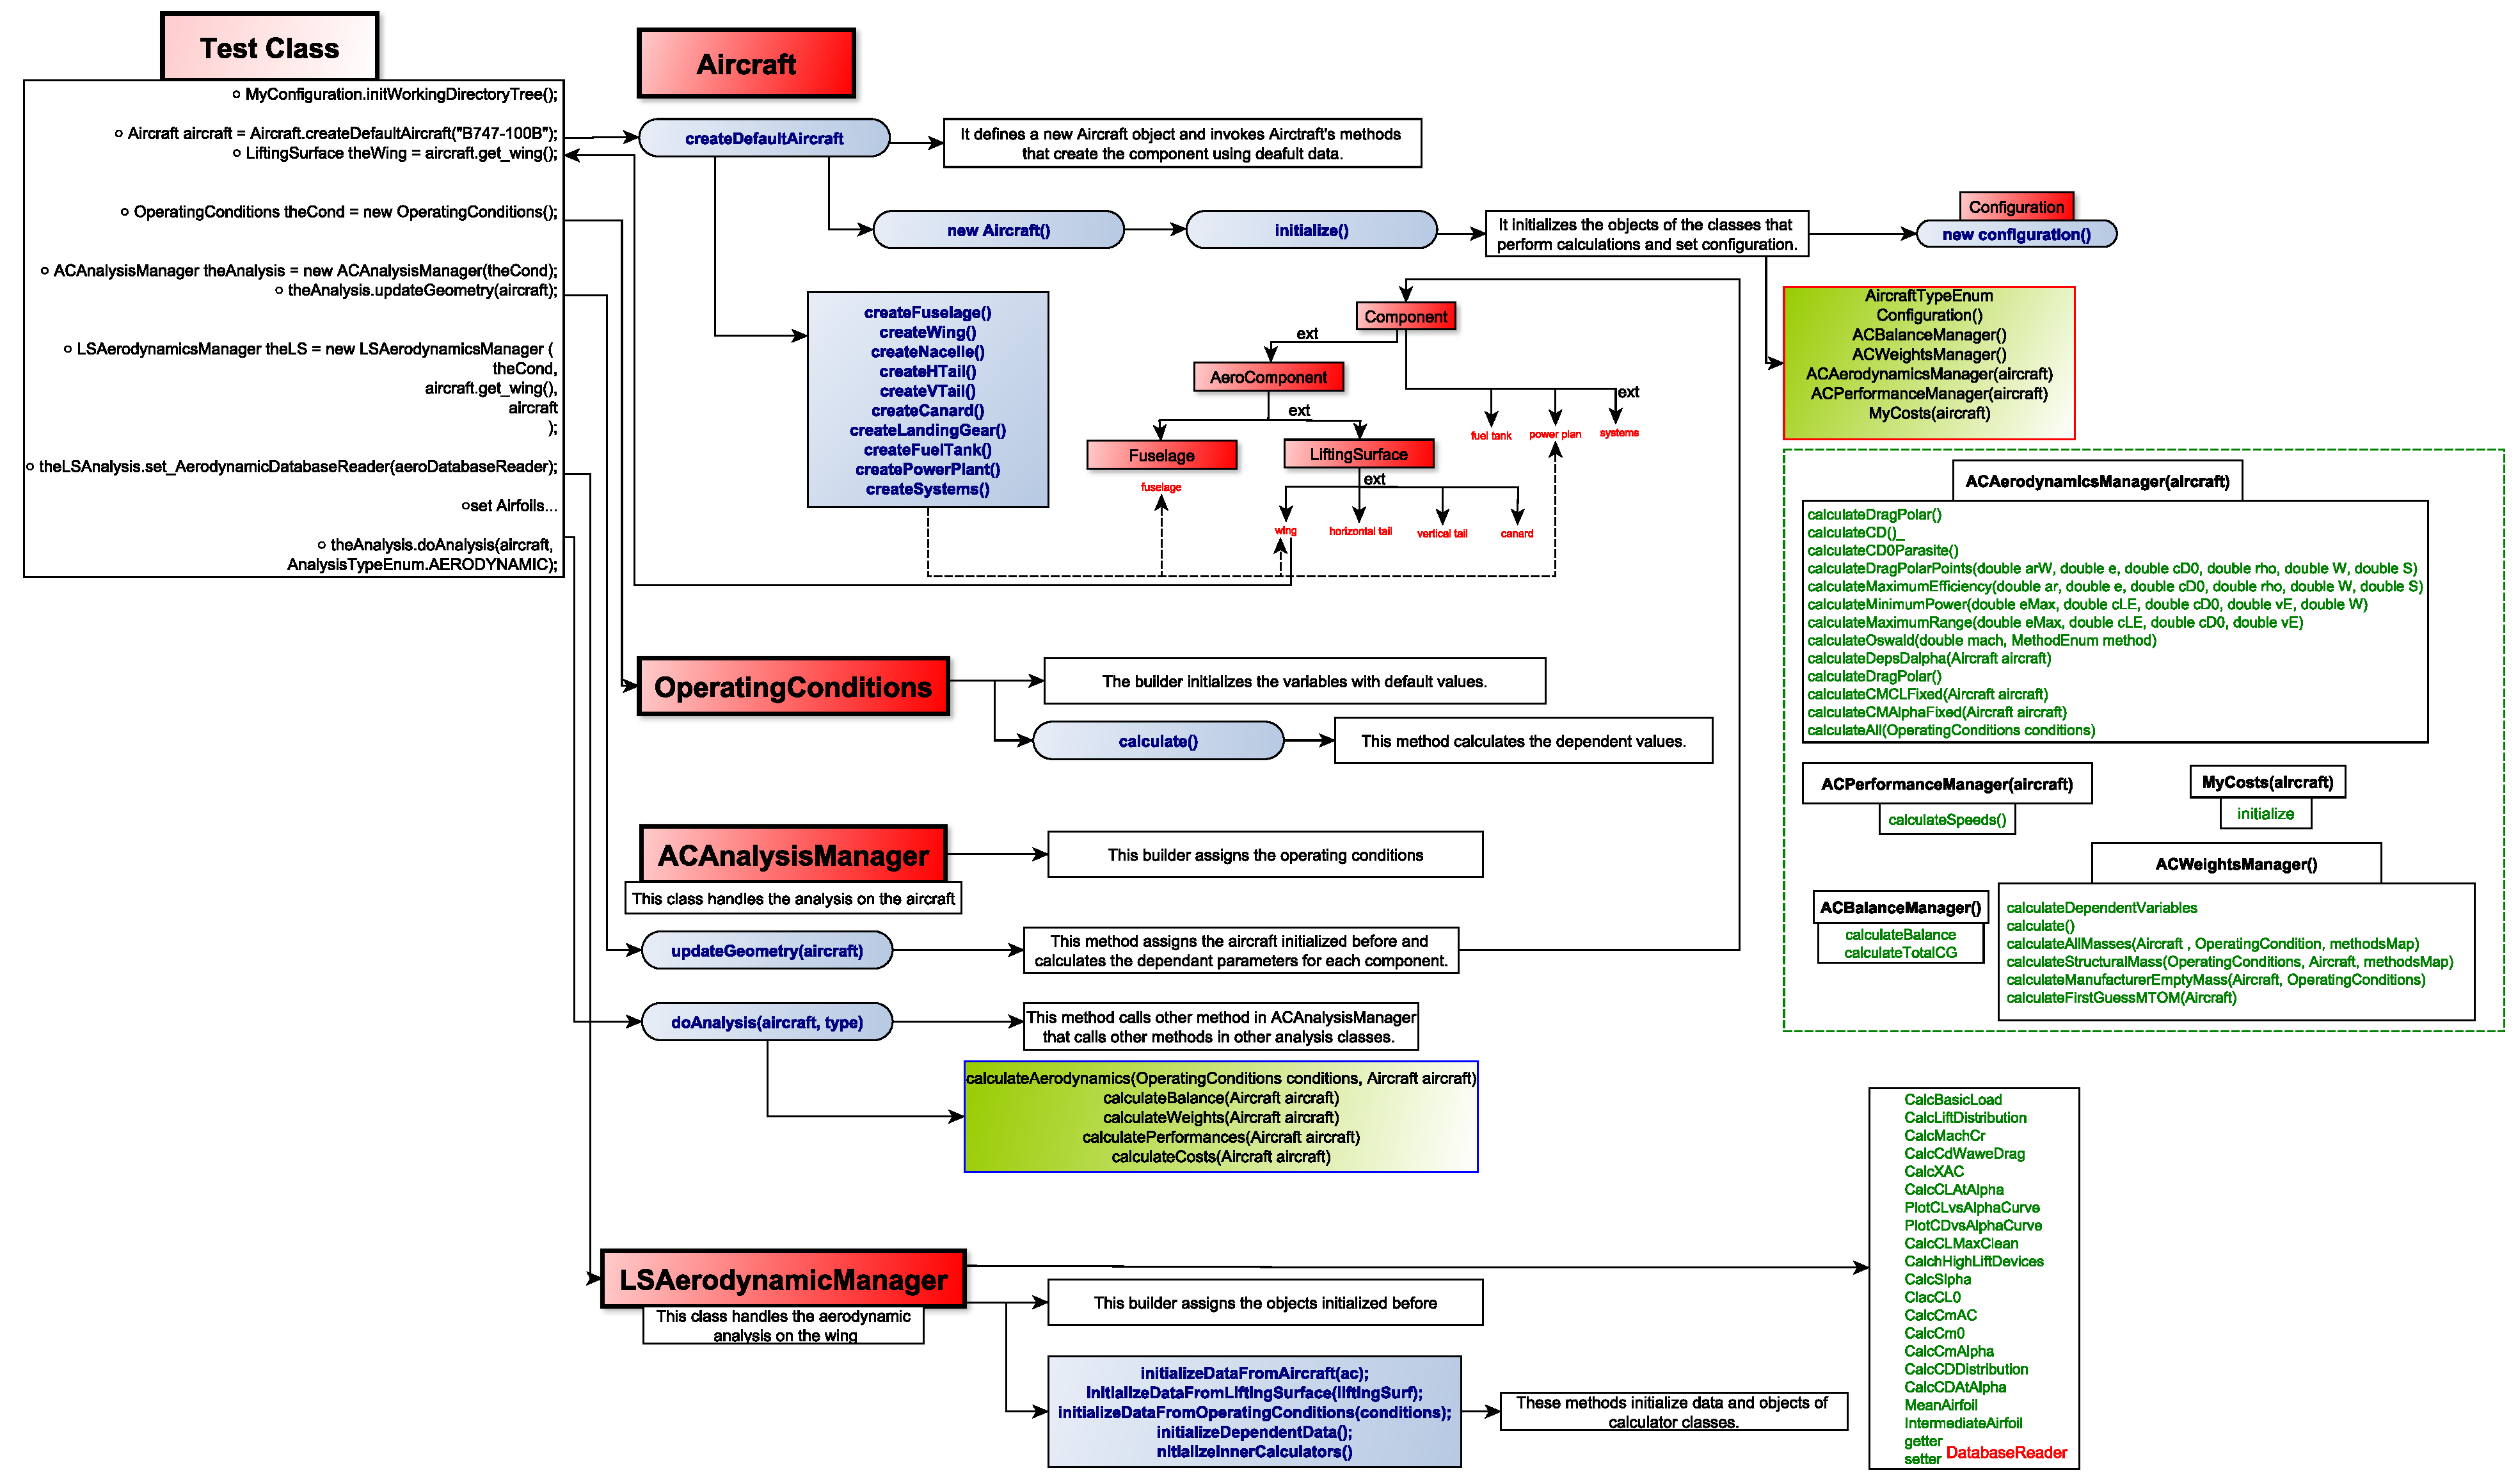
\includegraphics[width=24.6cm]{immagini/HowToCreateADefaultAircraftInJPAD3.pdf}
\caption{Flow chart of the creation of default Aircraft.}
\label{fig:schemauno}

\end{sidewaysfigure}

\subsection {How is made a default Wing}
Similary to the default aircraft it is possible to define a default wing. This is very useful if the user wants to make an analysis only on a wing. In this case it is necessary to define the origin of the \gls{acr:lrf} in \gls{acr:brf} and the coordinates of the \gls{acr:cg}.\\
Contrary to the case of the aircraft, for an isolated wing it is not necessary to define a fuselage in order to create a \texttt{Lifting Surface} object, but there is an overload of the builder that does not need a fuselage as input. In this case the exposed surface is calculated as the surface of the wing.

\noindent \\
\begin{lstlisting}[frame=rbl,caption={{\footnotesize Generation of an isolated Wing}},label= [style=\bfseries]{Listing}]
public static void main(String[] args) {

	// Assign all default folders
	MyConfiguration.initWorkingDirectoryTree();
	
	// -----------------------------------------------------------------------
	// Coordinates of LRF
	// -----------------------------------------------------------------------
	
	double xAw = 11.0; //meter 
	double yAw = 0.0;
	double zAw = 1.6;
	double iw = 0.0;
	
	// -----------------------------------------------------------------------
	// Generate default Wing
	// -----------------------------------------------------------------------
	
	LiftingSurface theWing = new LiftingSurface(
			"Wing", // name
			"Data from AC_ATR_72_REV05.pdf", 
			xAw, yAw, zAw, iw, 
			ComponentEnum.WING
			); 

	theWing.calculateGeometry();
	theWing.getGeometry().calculateAll();
	
	// -----------------------------------------------------------------------
	// Center of Gravity
	// -----------------------------------------------------------------------	
	
	double xCgLocal= 1.5; // meter 
	double yCgLocal= 0;
	double zCgLocal= 0;

	CenterOfGravity cg = new CenterOfGravity(
			Amount.valueOf(xCgLocal, SI.METER), // coordinates in LRF
			Amount.valueOf(yCgLocal, SI.METER),
			Amount.valueOf(zCgLocal, SI.METER),
			Amount.valueOf(xAw, SI.METER), // origin of LRF in BRF 
			Amount.valueOf(yAw, SI.METER),
			Amount.valueOf(zAw, SI.METER),
			Amount.valueOf(0.0, SI.METER),// origin of BRF
			Amount.valueOf(0.0, SI.METER),
			Amount.valueOf(0.0, SI.METER)
			);

	cg.calculateCGinBRF();
	theWing.set_cg(cg);
	theWing.set_aspectRatio(6.0);

	// Default operating conditions
	OperatingConditions theOperatingConditions = new OperatingConditions();		
	theOperatingConditions.set_alphaCurrent(Amount.valueOf(2.0, NonSI.DEGREE_ANGLE)

	// --------------------------------------------------------------
	// Define an LSAerodynamicsManager Object
	// --------------------------------------------------------------
	
	LSAerodynamicsManager theLSAnalysis = new LSAerodynamicsManager ( 
			theOperatingConditions,
			theWing
			);

	// --------------------------------------------------------------
	// Setup database(s)	
	// --------------------------------------------------------------
	
	theLSAnalysis.setDatabaseReaders(
			new Pair(DatabaseReaderEnum.AERODYNAMIC, 
					"Aerodynamic_Database_Ultimate.h5"),
			new Pair(DatabaseReaderEnum.HIGHLIFT, "HighLiftDatabase.h5")
			);
	
	// --------------------------------------------------------------
	// Assign Airfoil(s) ...	
	// --------------------------------------------------------------

	  // Define airfoilRoot...
	
	// --------------------------------------------------------------
	// Set Airofoil(s)	
	// --------------------------------------------------------------
	List<MyAirfoil> myAirfoilList = new ArrayList<MyAirfoil>();
	myAirfoilList.add(0, airfoilRoot);
	myAirfoilList.add(1, airfoilKink);
	myAirfoilList.add(2, airfoilTip);
	theWing.set_theAirfoilsList(myAirfoilList);
	theWing.updateAirfoilsGeometry(); 
	theLSAnalysis.initializeDependentData();

}
\end{lstlisting}

\section {Database in JPAD}

In JPAD it is possible to consult external databases in .h5 format. {\bfseries HDF 5} (Hierarchical Data Format Release 5) is a data file format designed by the {\itshape National Center for Supercomputing Applications} (NCSA) to assist users in the storage and manipulation of scientific data across different operating systems and machines.\\
To obtain the useful data in JPAD  interpolating functions are used . These functions can be of one, two or three dimensions and read data from graphics that have been digitize previously.\\
Starting from these digitalizations, databases in .h5 format are built.
Reading data from databases is entrusted to methods of classes in the \texttt{database} package.\\
In order to read these databases, and obtain the useful data, it is necessary to define an object of the database reading class and associate it with the object of analysis.\\
This is a crucial step to read correctly the external data. Infact JPAD allows to work with an aircraft object  or only with an isolated lifting surface object.  Aircraft is usually composed of a fuselage, lifting surfaces, nacelle and power plant.
Furthermore, \texttt{Aircraft} and \texttt{Wing} are associated with classes of calculation like \texttt{LSAerodynamicManager} or \texttt{ACAnalysisManager}. So it is necessary that these databases are also visible from these classes.\\
So because both in the aircraft and in the wing there is a lifting surface object, databases relative to wing are associated to \texttt{LSAerodynamicManager}.

\subsection {Setup database}
Here the database path is created and associated to object that interpolates the required data from the .h5 file using a \texttt{MyInterpolatingFunction} object. After this it is possible to access the double value of the interpolating function using the \texttt{standaloneutils} method called \texttt{value}. \\


%\begin{lstlisting}[frame=rbl,caption={{\footnotesize Setup database(s)}},label= [style=\bfseries]{Listing}]
%// --------------------------------------------------------------
%// Define database
%// --------------------------------------------------------------
%MyConfiguration.initWorkingDirectoryTree();
%
%// Setup database(s)	
%String databaseFolderPath = MyConfiguration.getDir(FoldersEnum.DATABASE_DIR);
%String databaseFileName = "Aerodynamic_Database_Ultimate.h5";
%AerodynamicDatabaseReader aeroDatabaseReader = 
%		new AerodynamicDatabaseReader(
%				databaseFolderPath, 
%				databaseFileName
%				);
%\end{lstlisting}

Now the procedure to assign the database is different if is used an Aircraft object or a Wing object.

\subsection {Assign database using an Aircraft object}
In order to assign correctly the database and associate it to all analysis management is necessary to practise the following order.
\begin{enumerate}
\item Define an Aircraft Object.\\This command associates to the Aircraft an object that defines the aerodynamic. Defining an Aircaft object is defined the Wing, that is a \texttt{LiftingSurface} object.
\item Define an \texttt{ACAnalysisManager} object.\\All the aircraft computations are managed by this class.
\item Define an \texttt{LSAerodynamicManager} object.\\ All the lifting surfaces computations are managed by this class.
\item Associate database to \texttt{LSAerodynamicManager}.
\item Eventually do analysis.
\end{enumerate}

\subsection {Assign database using a Wing object}
Using a Wing object it is not necessary to define a manager for Aircraft aerodynamic analysis. So the step to follow are the same of aircraft starting from the third.
\begin{enumerate}
\item Define a Wing Object.
\item Define an \texttt{LSAerodynamicManager} object.
\item Associate database to \texttt{LSAerodynamicManager}.
\end{enumerate}

The definition of an isolated Wing is explained in the relative section.

%\begin{lstlisting}[frame=rbl,caption={{\footnotesize Assign database using an Aircraft object}},label= [style=\bfseries]{Listing}]
%
%// --------------------------------------------------------------
%// Generate default Aircraft
%// --------------------------------------------------------------
%Aircraft aircraft = Aircraft.createDefaultAircraft("B747-100B");
%LiftingSurface theWing = aircraft.get_wing();
%		
%// Default operating conditions
%OperatingConditions theConditions = new OperatingConditions();		
%		
%		
%// --------------------------------------------------------------
%// Define an ACAnalysisManager Object
%// --------------------------------------------------------------
%ACAnalysisManager theAnalysis = new ACAnalysisManager(theConditions);
%theAnalysis.updateGeometry(aircraft);
%		
%		
%// --------------------------------------------------------------
%// Define an LSAerodynamicsManager Object
%// --------------------------------------------------------------
%LSAerodynamicsManager theLSAnalysis = new LSAerodynamicsManager ( 
%		theConditions,
%		theWing,
%		aircraft
%		);
%		
%		
%// --------------------------------------------------------------
%// Associate database to LSAerodynamicManager
%// --------------------------------------------------------------
%theLSAnalysis.set_AerodynamicDatabaseReader(aeroDatabaseReader);
%
%		
%// --------------------------------------------------------------
%// Do analysis
%// --------------------------------------------------------------
%theAnalysis.doAnalysis(aircraft, 
%		AnalysisTypeEnum.AERODYNAMIC);
%\end{lstlisting}

\noindent \\
\begin{lstlisting}[frame=rbl,caption={{\footnotesize Assign database using an Aircraft object}},label= [style=\bfseries]{Listing}]
		
	// --------------------------------------------------------------
	// Setup database(s)	
	// --------------------------------------------------------------
		
	theLSAnalysis.setDatabaseReaders(
			new Pair(DatabaseReaderEnum.AERODYNAMIC,
                          "Aerodynamic_Database_Ultimate.h5"),
			new Pair(DatabaseReaderEnum.HIGHLIFT,  
                          "HighLiftDatabase.h5")
			);

\end{lstlisting}
The databases are assigned to \texttt{LSAerodynamic} using a method of this class. This method accept as input a variable number of \texttt{Pair} objects.Using \texttt{Pair} objects it is possible to assign, for each database, both name and type. 

\noindent \\
\begin{lstlisting}[frame=rbl,caption={{\footnotesize \texttt{setDatabaseReaders} method}},label= [style=\bfseries]{Listing}]

public void setDatabaseReaders(Pair... args) {
	String databaseFolderPath = MyConfiguration.getDir(FoldersEnum.DATABASE_DIR);
	
	for (Pair a : args) {
		DatabaseReaderEnum key = (DatabaseReaderEnum)a.getKey(); 
		String databaseFileName = (String)a.getValue();
		
		switch (key) {
			case AERODYNAMIC:
				_aerodynamicDatabaseReader = 
				new AerodynamicDatabaseReader(
						databaseFolderPath,
						databaseFileName); 
				listDatabaseReaders.add(_aerodynamicDatabaseReader);
				break;
				
			case HIGHLIFT:
				_highLiftDatabaseReader = 
				new HighLiftDatabaseReader(
						databaseFolderPath, 
						databaseFileName); 
				listDatabaseReaders.add(_highLiftDatabaseReader);
			break;	
			
		}
\end{lstlisting}


\subsection {User's guide}

In order to execute some analysis in JPAD it is necessary, first of all, to define an analysis object in the Test class. The method \texttt{createDefaultAircraft} creates a new aircraft and the object that composes it. This method also populates the data of aircraft with default value corresponding to ATR-72 or Boieng 747-100B. Moreover the method \texttt{createDefaultAircraft} calls another method in \texttt{Aircraft} class: \texttt{initialize} that initializes the objects of the classes that perform calculations. \\
The purpose of this structure is to have only a way to assign the databases at an aircraft. Inasmuch as the wing is always present, the chosen strategy is to assign the database to the aerodynamic manager of the wing.\\
In order to bring to use the database also for the aircraft calculation, it is assigned at the aerodynamic manager of the aircraft in the method called \texttt{doAnalysis}.\\
At the same time \texttt{LSAerodynamicManager} sets itself as aerodynamic in the wing object. \\
So it is possible to call the database using equally the following codes: 
\begin{itemize}
\item \texttt{theWingObject.getAerodynamics.get\_Database;}
\item \texttt{theAircraftObject.get\_theAerodynamic.get\_Database;}
\item \texttt{theLSManagerObject.get\_Database;}
\item \texttt{theACManagerObject.get\_Database;}
\end{itemize}

\begin{sidewaysfigure}

\centering
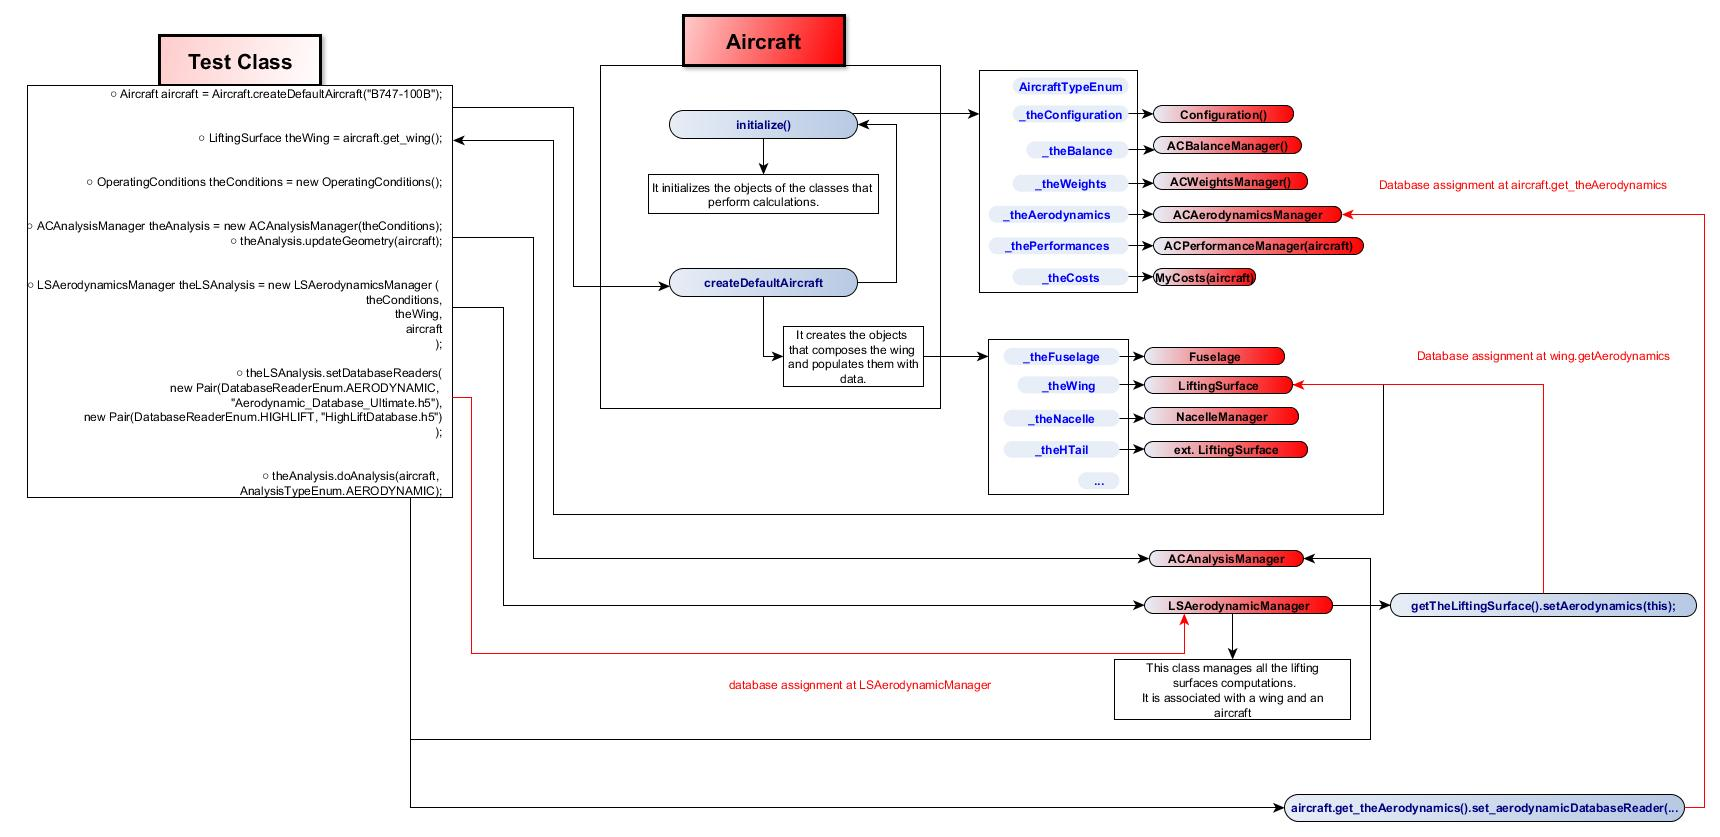
\includegraphics[width=23cm]{immagini/HowToAssignDatabase.jpg}
\caption{Flow chart of database assignment.}
\label{fig:schemauno}

\end{sidewaysfigure}

\part{Functionality Overview}
\chapter{Wing Lift Characteristics}
\label{ch:workobject}
\markboth{Wing Lift Characteristics}{}

\begin{flushright}
	{\smaller
		\textit{Citazione\\ citazione}\\
		-- Autore}
\end{flushright}


Any body in motion in a fluid presents a result of force acting on it, which can be decomposed in two components:
\begin{itemize}
\item A {\bfseries Lift} acting normal to the Velocity direction and is positive upward.
\item A {\bfseries Drag} acting in the opposite direction to the airspeed vector.
\end{itemize}
The lifting surfaces of an airplane are designed to generate lift exceeding their drag, in order to obtain a positive efficiency.
\chapter{Wing Drag Characteristics}

\label{ch:wingdrag}
\markboth{Wing Drag Characteristics}{}

\begin{flushright}
	{\smaller
		\textit{It is not certain\\ that everything is uncertain}\\
		-- Blaise Pascal}
\end{flushright}


As mentioned in the previous chapter, the drag is the force component acting in the opposite direction to the airspeed vector.\\
There isn't a single classification of the drag but, dependent on the purpose of the work, the drag may be broken down in different way. Following will be explained the two main classifications.

\begin{itemize}
\item The drag is subdivided using a causal breakdown. In this way the drag contributes are in accordance with the physical mechanism such as the viscosity of the flow.
\item The drag is subdivided using a component breakdown. Every component of aircraft added an own drag contribute.
\end{itemize}

\begin{figure}[H]
\centering
{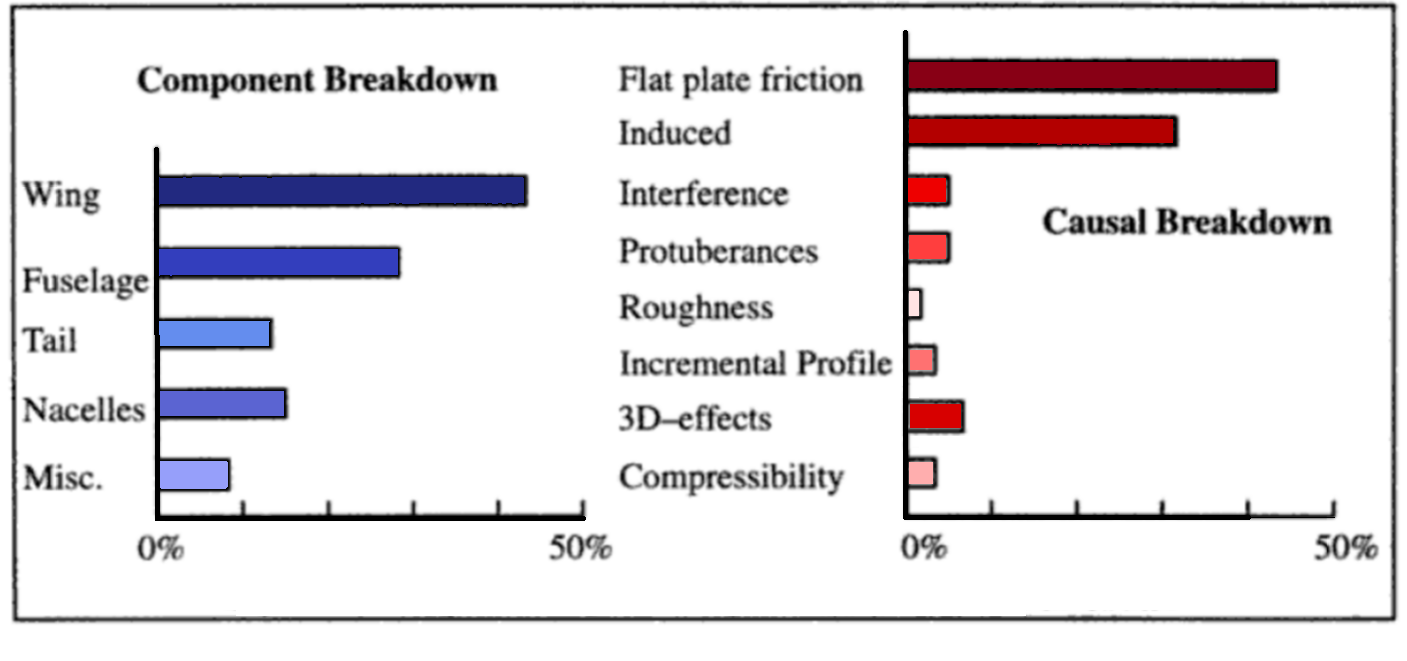
\includegraphics[height=6.4cm]{Immagini/component.png}} 
\caption{Drag breakdown for a business jet in cruise.}
\end{figure}

According to the casual breakdown it's possible to make a preliminary division considering normal and tangential stress. The tangential forces produce the {\bfseries friction drag}. While it's possible to divide the drag due of the normal component in viscous, that generates {\bfseries form drag}, and inviscid. A further division can be made for the last one, in {\bfseries induced drag}  and {\bfseries wave drag}.\\

\begin{figure}[H]
\centering
{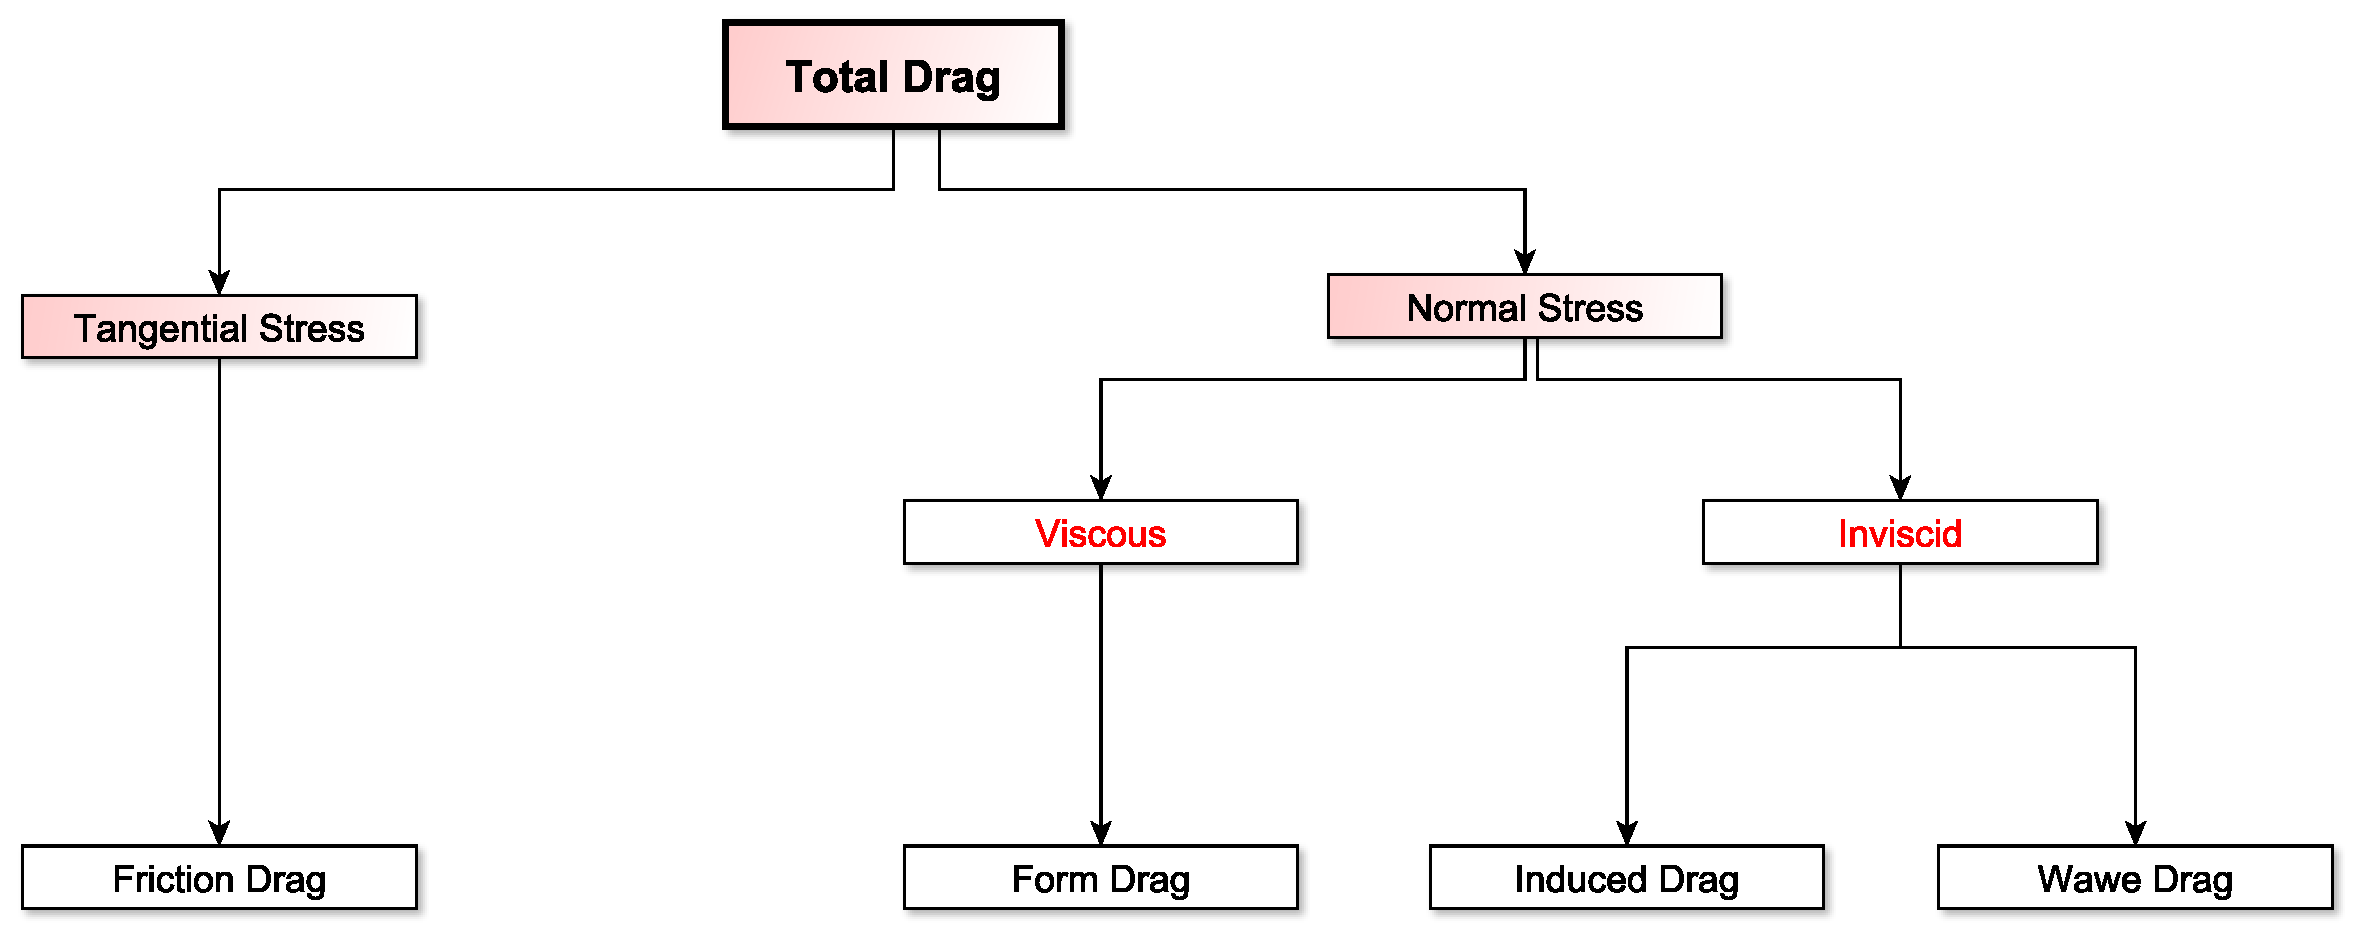
\includegraphics[height=6cm]{Immagini/dragcausal.pdf}} 
\caption{Causal breakdown of airplane drags.}
\end{figure}


Friction drag is caused by the air closest to the body’s surface that is dragged along with it. Due to this interaction shearing stresses are born within the thin layer of air (boundary layer) adiacent to the skin. The magnitude of this drag depends on the kind of boundary layer what can be laminar or turbulent in dependence on the Raynolds number. Usually it's accustomed to assume, at the flight speed and altitudes at which aircraft fly, a fully turbulent flow over the entire airplane. In this way a conservative result is obtained.\\
Form drag is caused by the air that is flowing over the body. The separation of air creates turbulence and results in pockets of low and high pressure that leave a wake behind the airplane. The departure of the boundary layer alters the pressure field from its inviscid distribution resulting in an additional drag component. The general size and shape of the body are the most important factors in form drag; bodies with a larger presented cross-section will have a higher drag than thinner bodies.\\
Induced drag is the drag due to lift. It is the drag created by the vortices at the tip of an aircraft's wing. The high pressure underneath the wing causes the airflow at the tips of the wings to curl around from bottom to top in a circular motion. So it's depend on the spanwise distribution of lift. \\
Wave drag is a component of the drag due to the presence of shock waves. Wave drag is independent of viscous effects, and tends to present itself as a sudden and dramatic increase in drag as the vehicle increases speed.
\\ \\ 
In this work the drag will be classified using a component breakdown. In this way it's possible to evaluate separately the wing drag and tail drag, considering the aerodynamic centers of these lifting surfaces as application point.

\begin{figure}[H]
\centering
{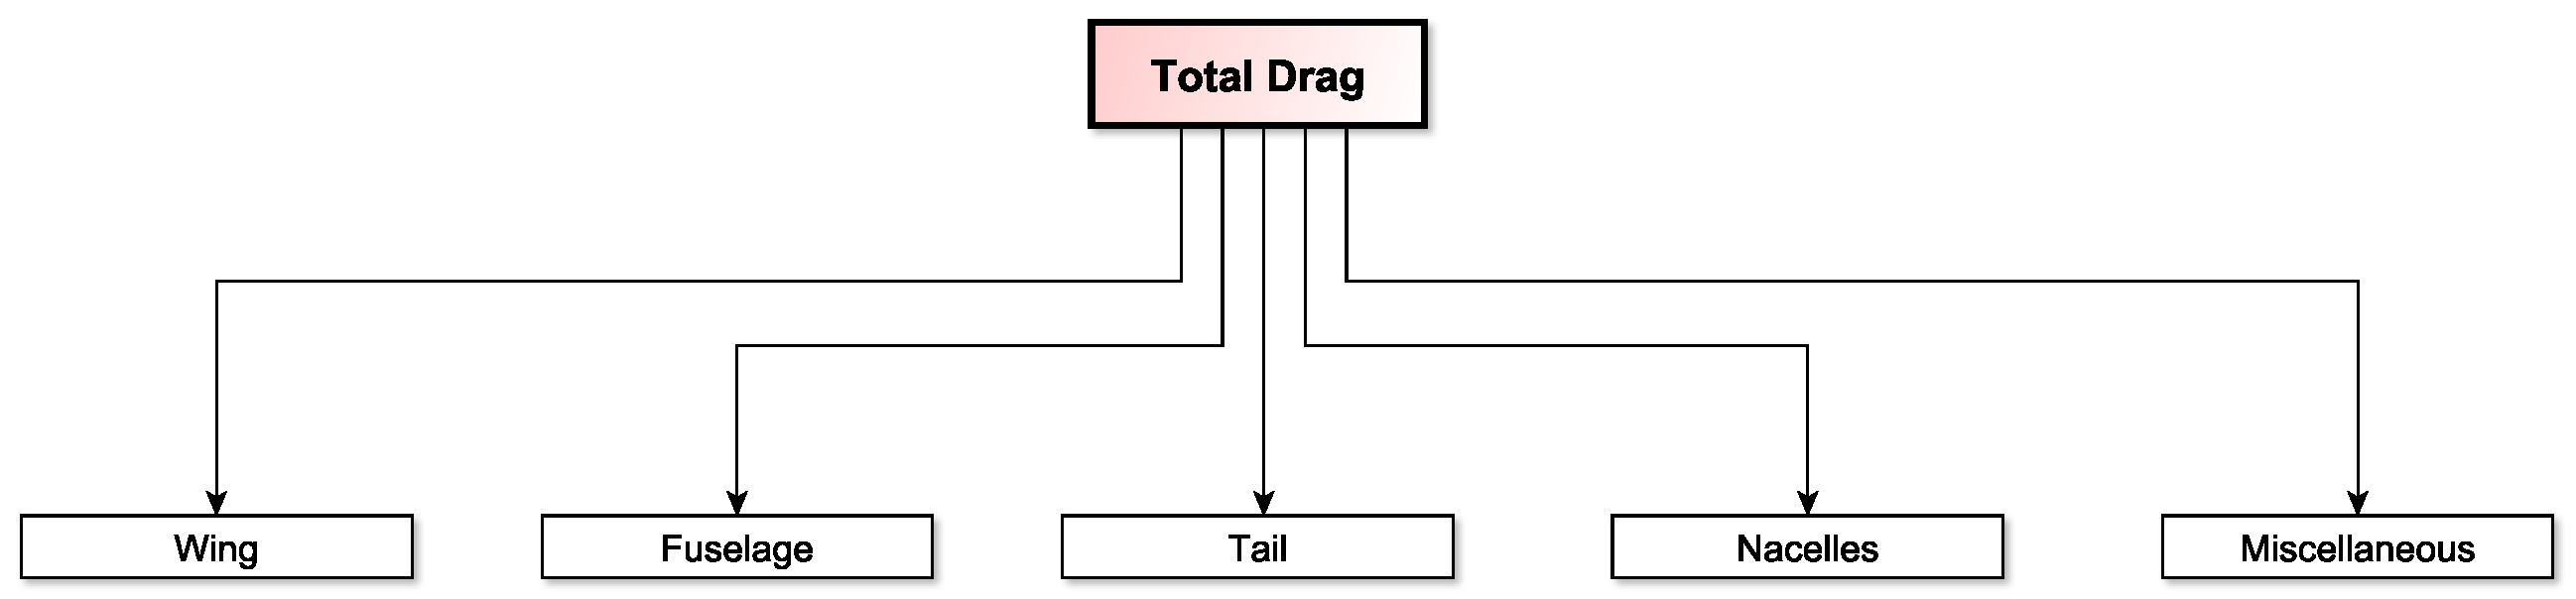
\includegraphics[height=3.6cm]{Immagini/dragco.pdf}} 
\caption{Components breakdown of airplane drags.}
\end{figure}

\section{Theoretical background}

In this thesis the drag coefficient of an isolated lifting surface is calculated starting from the load distribution and considering the parabolic approximation for the drag polar. The implemented process is the following:

\begin{enumerate}
\item First of all the load distribution at a given angle of attack has been calculated
\item Fifty points along the semispan are defined
\item For each point, an intermediate profile is calculated
\item To each profile correspond the lift coefficient at that station
\item Starting from the CL, using a parabolic approximation for the drag polar, the CD is calculated with the following equation
\begin{equation}
CD = CD_{min} + (CL - CL_{CD_{min}})^2 + k
\end{equation}
\item Known the drag distribution it is possible to calculate the drag coefficient of the lifting surface integrating
\end{enumerate}

In the tool it is possible to choose the method used to calculate the load distribution. In particular it's possible to use Shrenk or Nasa-Blackwell method.\\

{\bfseries Schrenk Method} is based on an elliptical lifting coefficient distribution span wise hypothesis on the wing. This method also assumes that the pressure distribution is proportional to the wing area. \\ 

The {\bfseries Nasa-Blackwell}, as mentioned, is a numerical method for calculating the subsonic load distribution for arbitrary lifting surface arrangements at a fixed angle of attack. \ref{ch:worklift}


\section{Java Class Architecture}


In order to give more flexibility to the code, the calculation of drag coefficient is made from three different class summarized in the folloving table.

\begin{table}[H]
\begin{tabular}{p{7cm}p{7.5cm}}
\toprule
\lstinline[language=Java]!integralFromCdAirfoil! & This method calculates the drag coefficient of the lifting surface using an integral and calling other method that fills the needed field. This is in the nested class \texttt{CalcCDAtAlpha}\\ \hline 
\lstinline[language=Java]!nasaBlackwell! &This method calculates drag distribution starting from the load distribution calculated with Nasa-Blackwell method and using a parabolic approximation for the drag polar.  This is in the nested class \texttt{CalcCdDistribution} \\ \hline 
\lstinline[language=Java]!nasaBlackwell! & This method calculates the drag coefficient of an airfoil having the lift coefficient and using a parabolic approximation.\\ 
\bottomrule
\end{tabular}
\caption{Methods for drag coefficient calculatorof a lifting surface.}
\label{table:Table2}
\end{table}

\begin{figure}[H]
\centering
{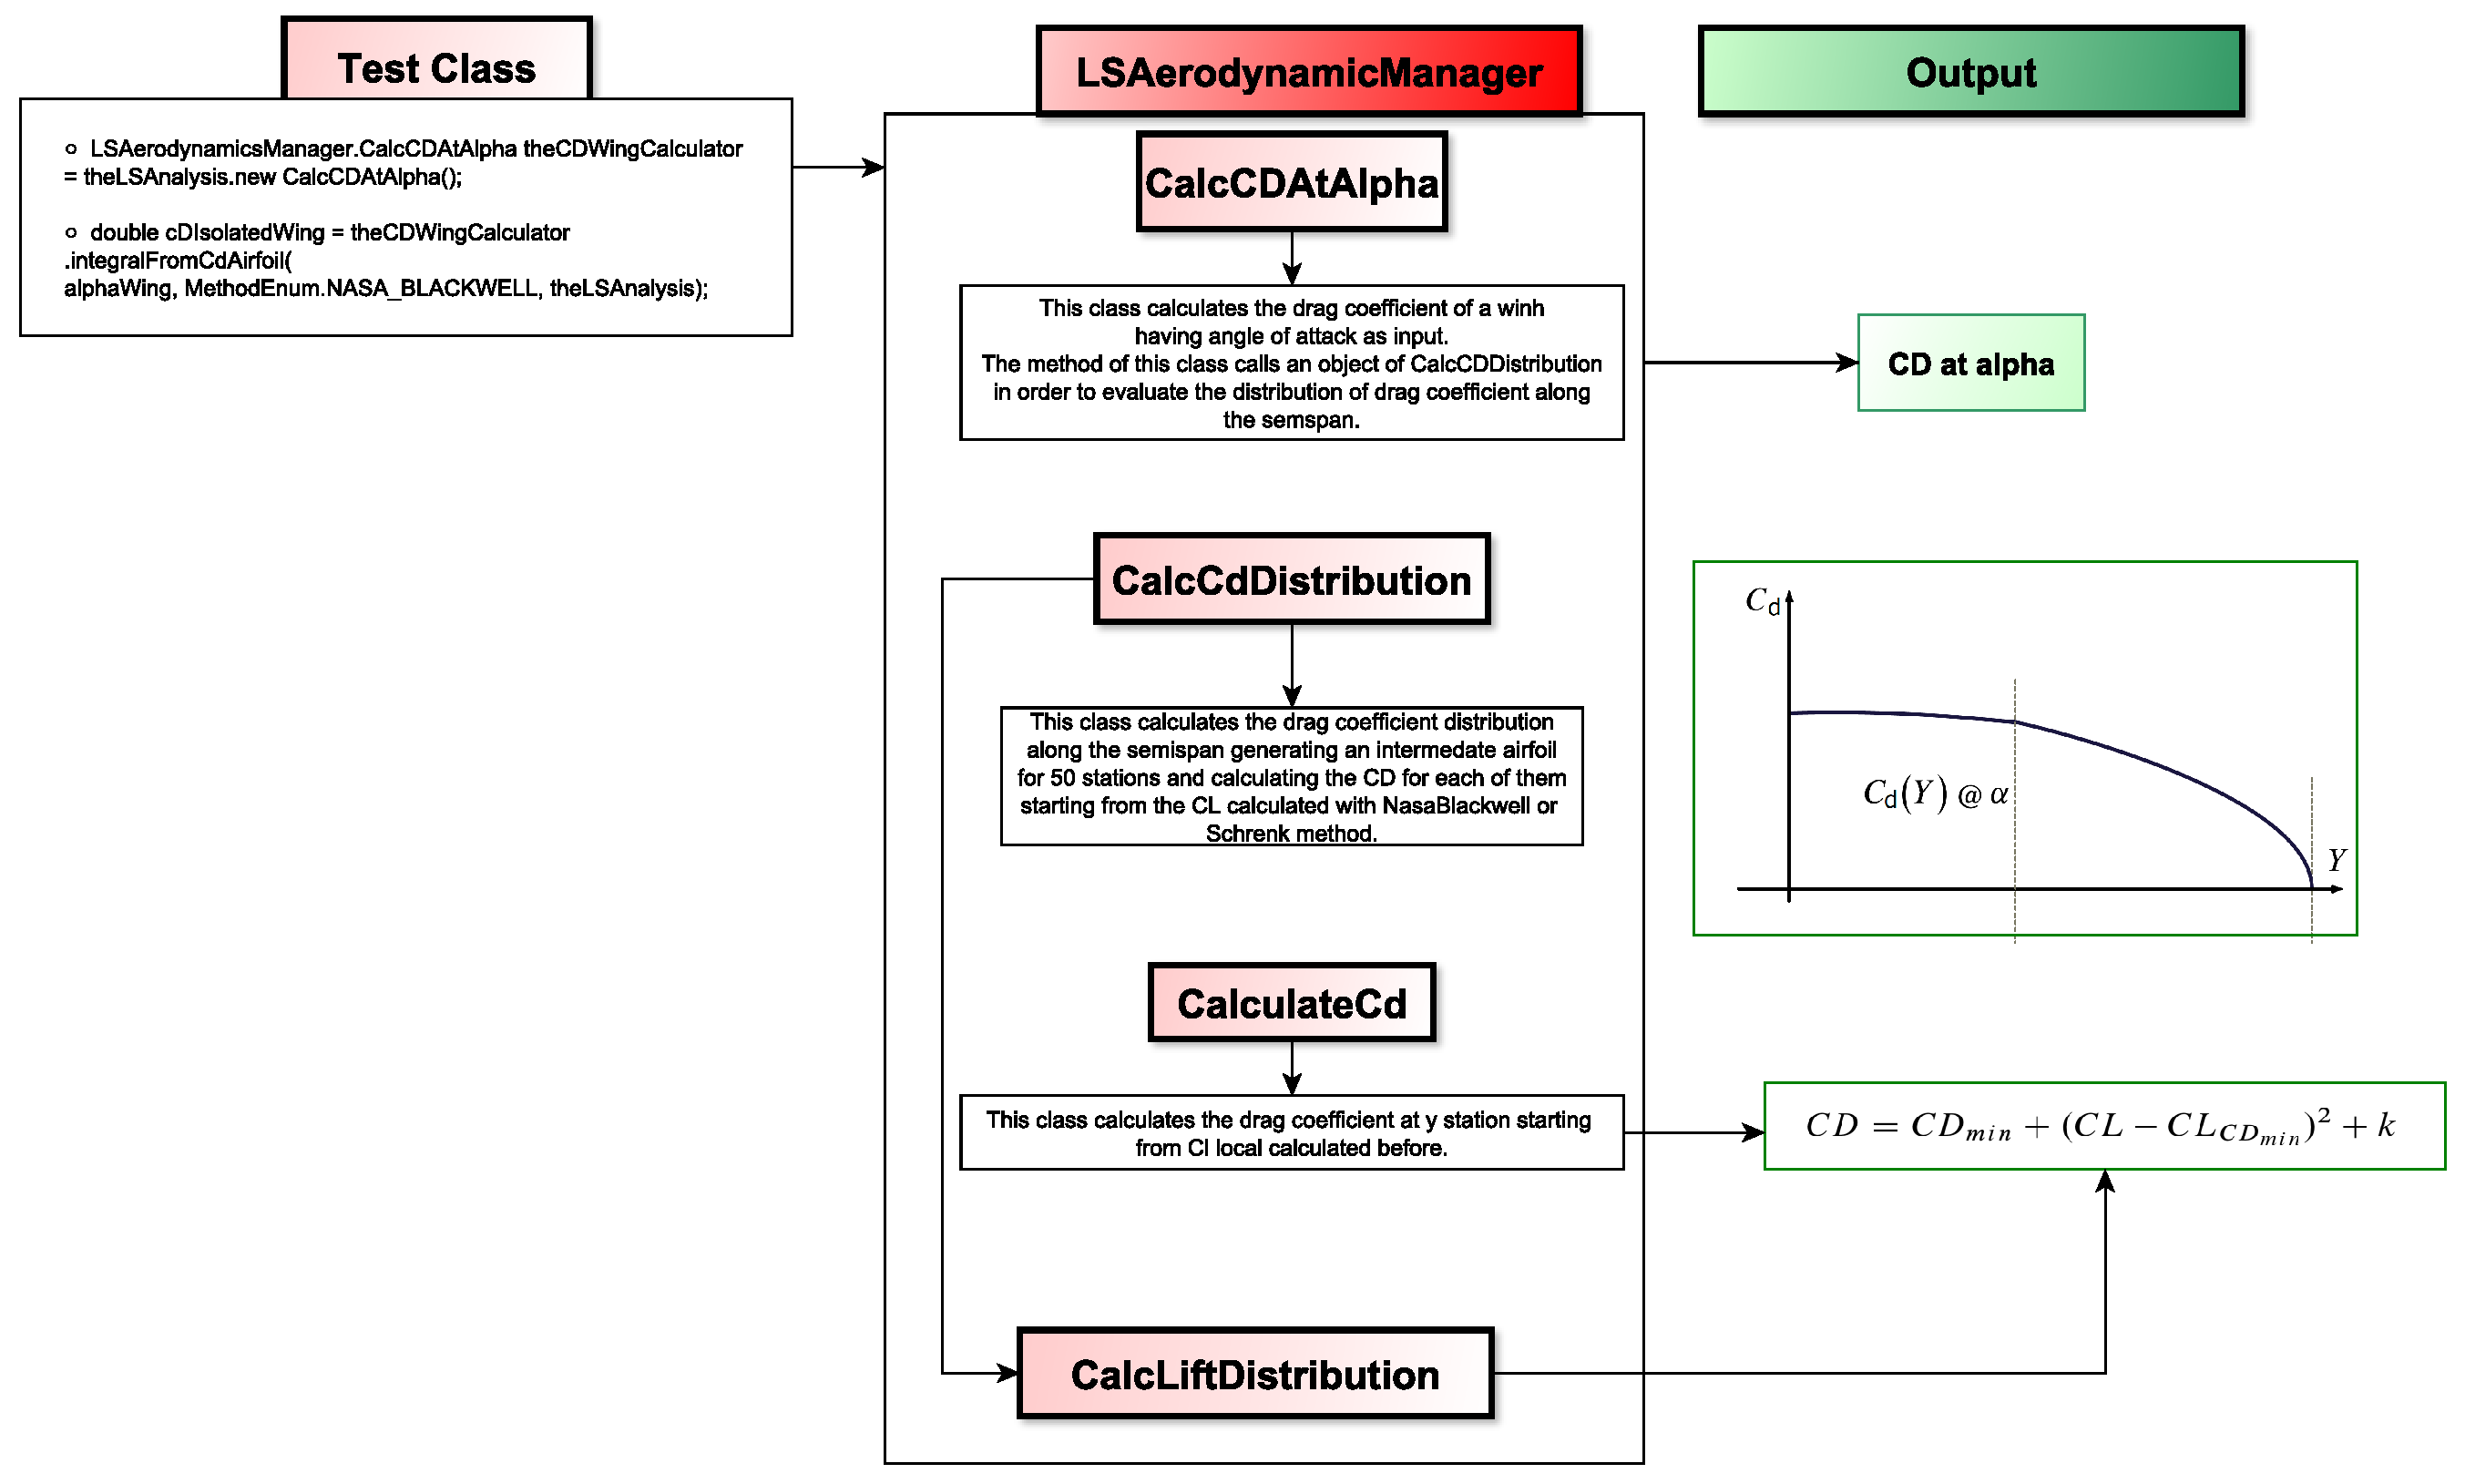
\includegraphics[height=9.9cm]{immagini/dragflowchart.pdf}}
\caption{Flow chart of drag estimation classes.}
\label{fig:Drag}
\end{figure}

\section{Case Study}

After initializing the Test class and defining the work object, it is possible to define an object of the class \texttt{CalcCDAtAlpha} that calculates the drag coefficient of a wing at a given angle of attack. This method accepts as input three parameters: the angle of attack of the wing,  the method used in order to calculate of lift distribution and an object of the lifting surface aerodynamic manager.\\
The it is possible to plot the curves of drag coefficient versus $\alpha_w$ or lift coefficient that is the drag polar of the wing.


\noindent \\
\begin{lstlisting}[frame=rbl,caption={{\footnotesize Use of Drag Calculator class}},label= [style=\bfseries]{Listing}]

// -----------------------------------------------------------------------
// DRAG CHARACTERISTICS 
// ----------------------------------------------------------------------

System.out.println("\n\n------------------------------------");
System.out.println("\n DRAG CHARACTERISTICS  ");
System.out.println("\n------------------------------------");

LSAerodynamicsManager.CalcCDAtAlpha theCDWingCalculator = theLSAnalysis
		.new CalcCDAtAlpha();
double cDIsolatedWing = theCDWingCalculator.integralFromCdAirfoil(
		alphaWing, MethodEnum.NASA_BLACKWELL, theLSAnalysis);
System.out.println(" CD of Wing at alpha body = (deg) "
		+ alphaBody.to(NonSI.DEGREE_ANGLE).getEstimatedValue()
		+ " is " + cDIsolatedWing);
	
System.out.println(" ...waiting for plotting");
theLSAnalysis.PlotCDvsAlphaCurve(subfolderPath);
System.out.println("\n\n\t\t\tDONE PLOTTING CD vs ALPHA WING");
			
}
\end{lstlisting}

\noindent \\

Following there are the summary diagrams of the results obtained for the ATR 72:

\noindent \\

\begin{figure}[H]
\centering
%CD vs Alpha WING
\begin{tikzpicture}

\begin{axis}[
width=14.01cm,
height=9cm,
scaled ticks=false, tick label style={/pgf/number format/fixed},
xmin=-2,
xmax=20,
xlabel={$\alpha_{w}$ (deg)},
xmajorgrids,
ymin=0,
ymax=0.24,
ylabel={CD},
ymajorgrids,
]

\addplot [
color=black,
thick
]
table[row sep=crcr]{
-2.0	0.011157714725733408\\
-1.3103448275862069	0.008954032848344878\\
-0.6206896551724137	0.00742401264401366\\
0.06896551724137945	0.006567654402364158\\
0.7586206896551726	0.006384957529857131\\
1.4482758620689657	0.00687592206936388\\
2.137931034482759	0.008040548557261913\\
2.827586206896552	0.009878836718217255\\
3.517241379310345	0.012390786552229914\\
4.206896551724139	0.015576398059299881\\
4.896551724137932	0.019435671239427164\\
5.586206896551726	0.023968611223650776\\
6.27586206896552	0.029175207619982896\\
6.965517241379313	0.035055445710204323\\
7.655172413793107	0.041609365722691374\\
8.3448275862069	0.048836966990760476\\
9.034482758620694	0.056738210174946714\\
9.724137931034488	0.06531311505609655\\
10.413793103448281	0.07456168163420986\\
11.103448275862075	0.08448390990928673\\
11.793103448275868	0.09507979988132707\\
12.482758620689662	0.10634935155033108\\
13.172413793103456	0.11829256491629847\\
13.862068965517249	0.13090943997922957\\
14.551724137931043	0.144199976739124\\
15.241379310344836	0.15816417519598194\\
15.93103448275863	0.17280203534980365\\
16.620689655172423	0.18811354703961328\\
17.310344827586217	0.20409873184511432\\
18.0	0.22075757842154453\\
};
\end{axis}
\end{tikzpicture}%

\caption{ATR 72 CD vs Alpha_w at Mach 0.43 and Altitude: 6000 m.}
\label{fig:DragATR}
\end{figure}


\begin{figure}[H]
\centering
%CD vs Alpha WING
\begin{tikzpicture}

\begin{axis}[
width=14.01cm,
height=9cm,
scaled ticks=false, tick label style={/pgf/number format/fixed},
xmin=0,
xmax=0.23,
xlabel={CD},
xmajorgrids,
ymin=-0.1,
ymax=2,
ylabel={CL},
ymajorgrids,
]

\addplot [
color=black,
thick
]
table[row sep=crcr]{
0.011157714725733408	-0.08006402986511459\\
0.008954032848344878	-0.012867908645348279\\
0.00742401264401366	0.05432821257441799\\
0.006567654402364158	0.12152433379418433\\
0.006384957529857131	0.18872045501395063\\
0.00687592206936388	0.25591657623371694\\
0.008040548557261913	0.32311269745348326\\
0.009878836718217255	0.3903088186732495\\
0.012390786552229914	0.45750493989301605\\
0.015576398059299881	0.5247010611127821\\
0.019435671239427164	0.5918971823325485\\
0.023968611223650776	0.6590933035523147\\
0.029175207619982896	0.7262894247720811\\
0.035055445710204323	0.7934855459918478\\
0.041609365722691374	0.8606816672116141\\
0.048836966990760476	0.9278777884313804\\
0.056738210174946714	0.9950739096511464\\
0.06531311505609655	1.062270030870913\\
0.07456168163420986	1.1294661520906797\\
0.08448390990928673	1.1966622733104453\\
0.09507979988132707	1.263858394530212\\
0.10634935155033108	1.3310545157499782\\
0.11829256491629847	1.3982506369697445\\
0.13090943997922957	1.4654467581895114\\
0.144199976739124	1.5326428794092772\\
0.15816417519598194	1.599839000629043\\
0.17280203534980365	1.6670351218488102\\
0.18811354703961328	1.7342312430685758\\
0.20409873184511432	1.801427364288343\\
0.22075757842154453	1.8686234855081083\\
};
\end{axis}
\end{tikzpicture}%

\caption{ATR 72 Parabolic Polar Drag at Mach 0.43 and Altitude: 6000 m.}
\label{fig:DragATR}
\end{figure}




\chapter{Downwash Estimation}

In order to evaluate the characteristics of longitudinal stability of an aircraft it's necessary to assess the flow direction aft of the wing. The contribution of horizontal tail surface to the airplane equilibrium and stability, in fact, depends seriously on the flow direction. The pourpose of this chapter is to introduce and evaluate the downwash gradient due from the wing's vortex system, considering a dipendence of the downwash angle from the absolute angle of attack. 

\section{Theoretical background}

Due to the finite extention of the wing the lift distribution in span is not uniform. For this reason the difference of pressure between upper and lower surfaces generates a movement of air aroud the wingtips. The tendency is for particles of air to move from the region of high pressure around the wing tip to the region of low pressure (for positive lift from the lower wing surface to the upper surface). This made the wing's vortex system that consisting of the bound vortex, located at the wing quarter chord and a vortex sheet which rolling up, at the wing tip, in two trailing vortex.\cite{PerkinsHage} \cite{Jacobs:NACA:Rep:648} \\ 

\begin{figure}[H]
\centering
{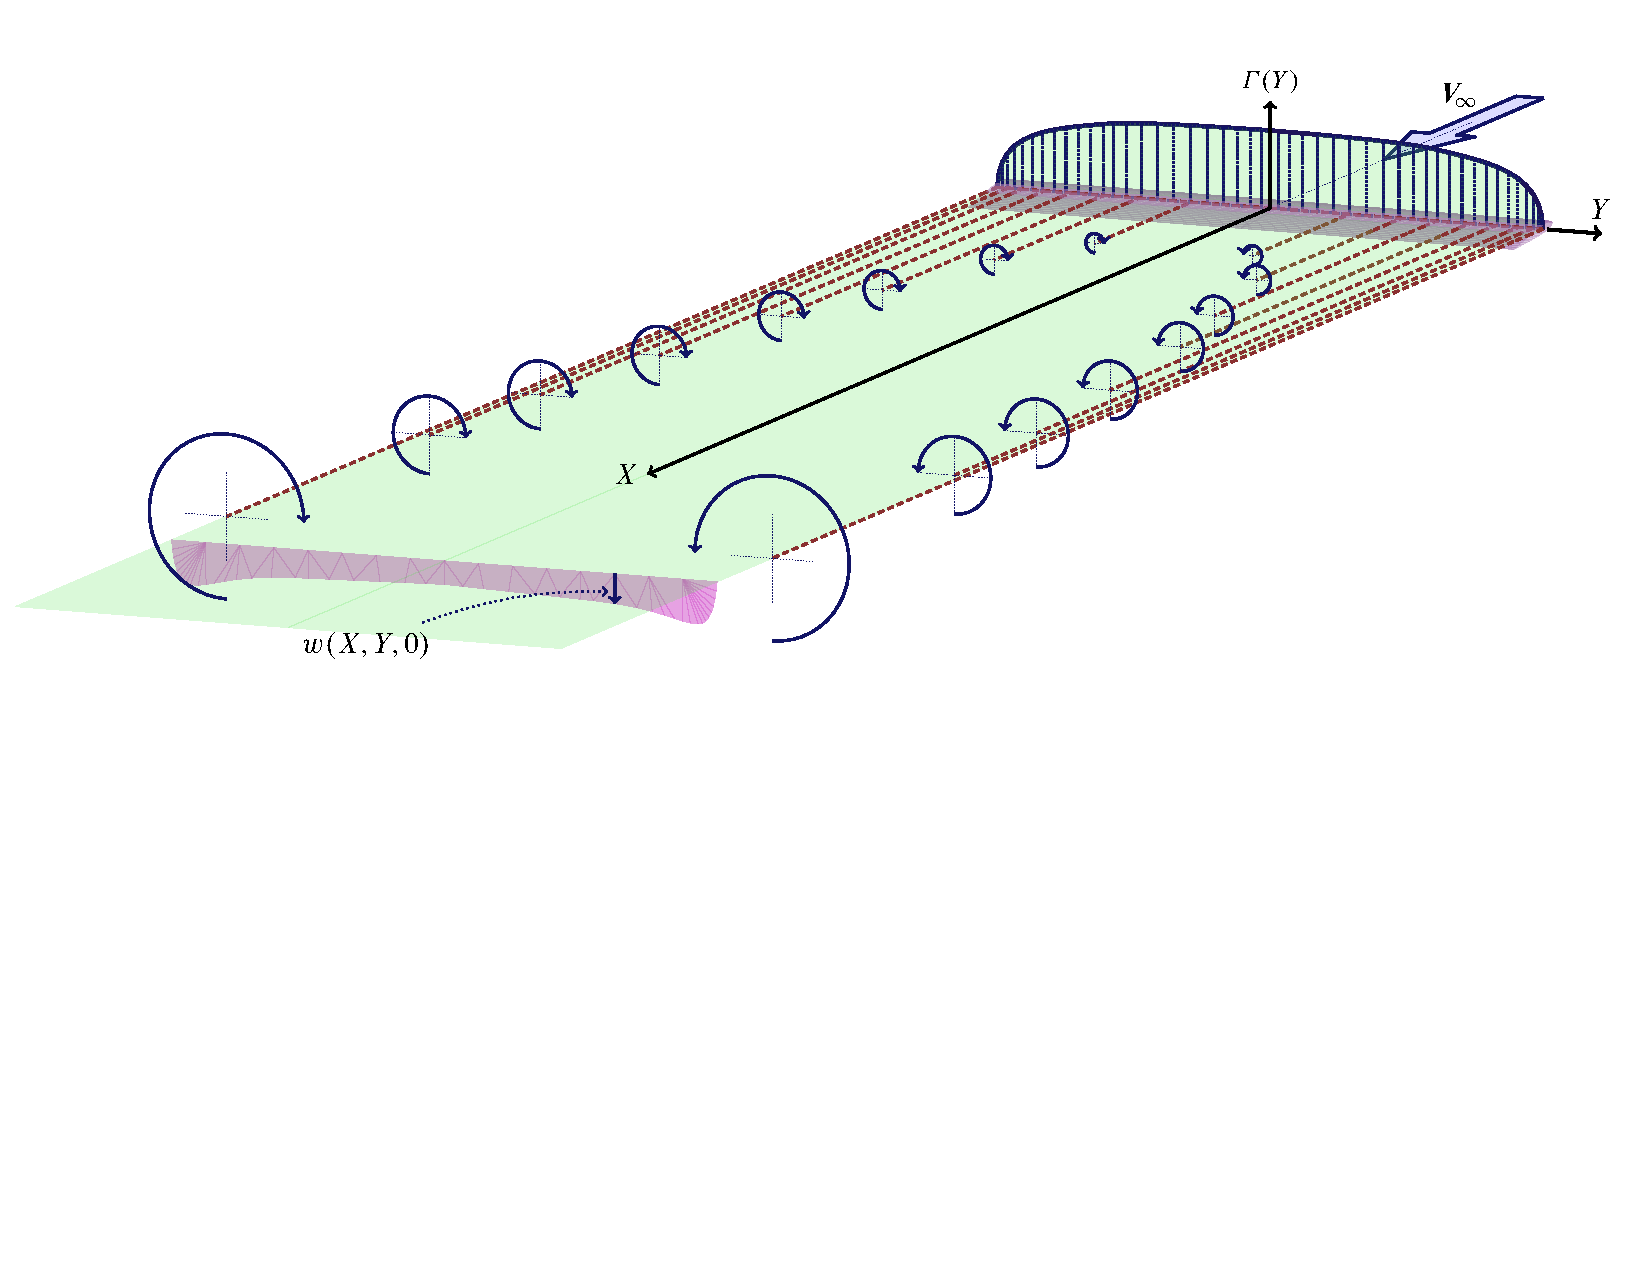
\includegraphics[height=6cm]{Immagini/wing_vortex_sheet3.pdf}} 
\caption{The wing vortex sheet.}
\end{figure}

The main effect of this vortex system is to deflect the airflow behind the wing downward relative to the direction of freestream flow. This angle of deviation is known as {\itshape Downwash Angle} $\epsilon$. This phenomenon occurs for every lifting surface, but in subsonic flow a lifting surface also affects the flow forward of itself. In this region the vortex creates an {itshape Upwash}, that is an upward flow deflection.\\


\begin{figure}[H]
\centering
{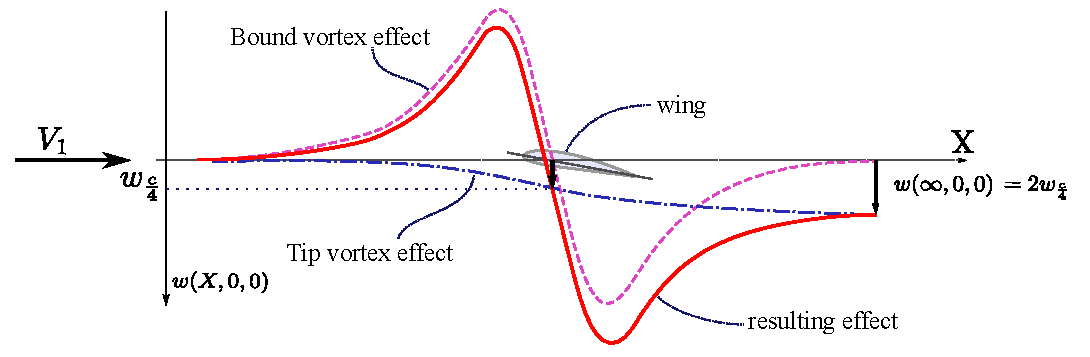
\includegraphics[height=5cm]{Immagini/wing_upwash_downwash.pdf}} 
\caption{Upwash and Downwash in a finite wing.}
\end{figure}

As consequence of the downwash behind the wing, the local angle of attack on the horizontal tail is reduced by  $\epsilon$. In order to evaluate the dlow direction behind the wing, an other important parameter id the change in downwash angle with angle of attack, that is the {\itshape Downwash Gradient } $\frac{d\epsilon}{d\alpha}$.\\
This parameter depends principally on the location of the horizontal tail with respect to the wing and the vortex plane. As first approssimation this value could be considered constant in alpha, but more accurately it's possible to evaluate this dependence considering the reference variable for the calculation of the distances. \\ \\

In order to evaluate the downwash gradient it refers to fig. \ref{PerkinsDownwash}, where ``$r \frac{b}{2}$''  is the distance between the aerodynamic center of wing and the aerodynamic center of the horizontal tail. This is a geometric an fixed distance. Conversely,  in order to have a greates accuracy it's possible to consider the distance ``$m  \frac{b}{2}$'' variable with the angle of attack. Properly this is the distance between the horizontal tail and the vortex shed plane, but it's possible to approximate it with the distance between the horizontal tail and the wing root chord.

\begin{figure}[H]
\centering
{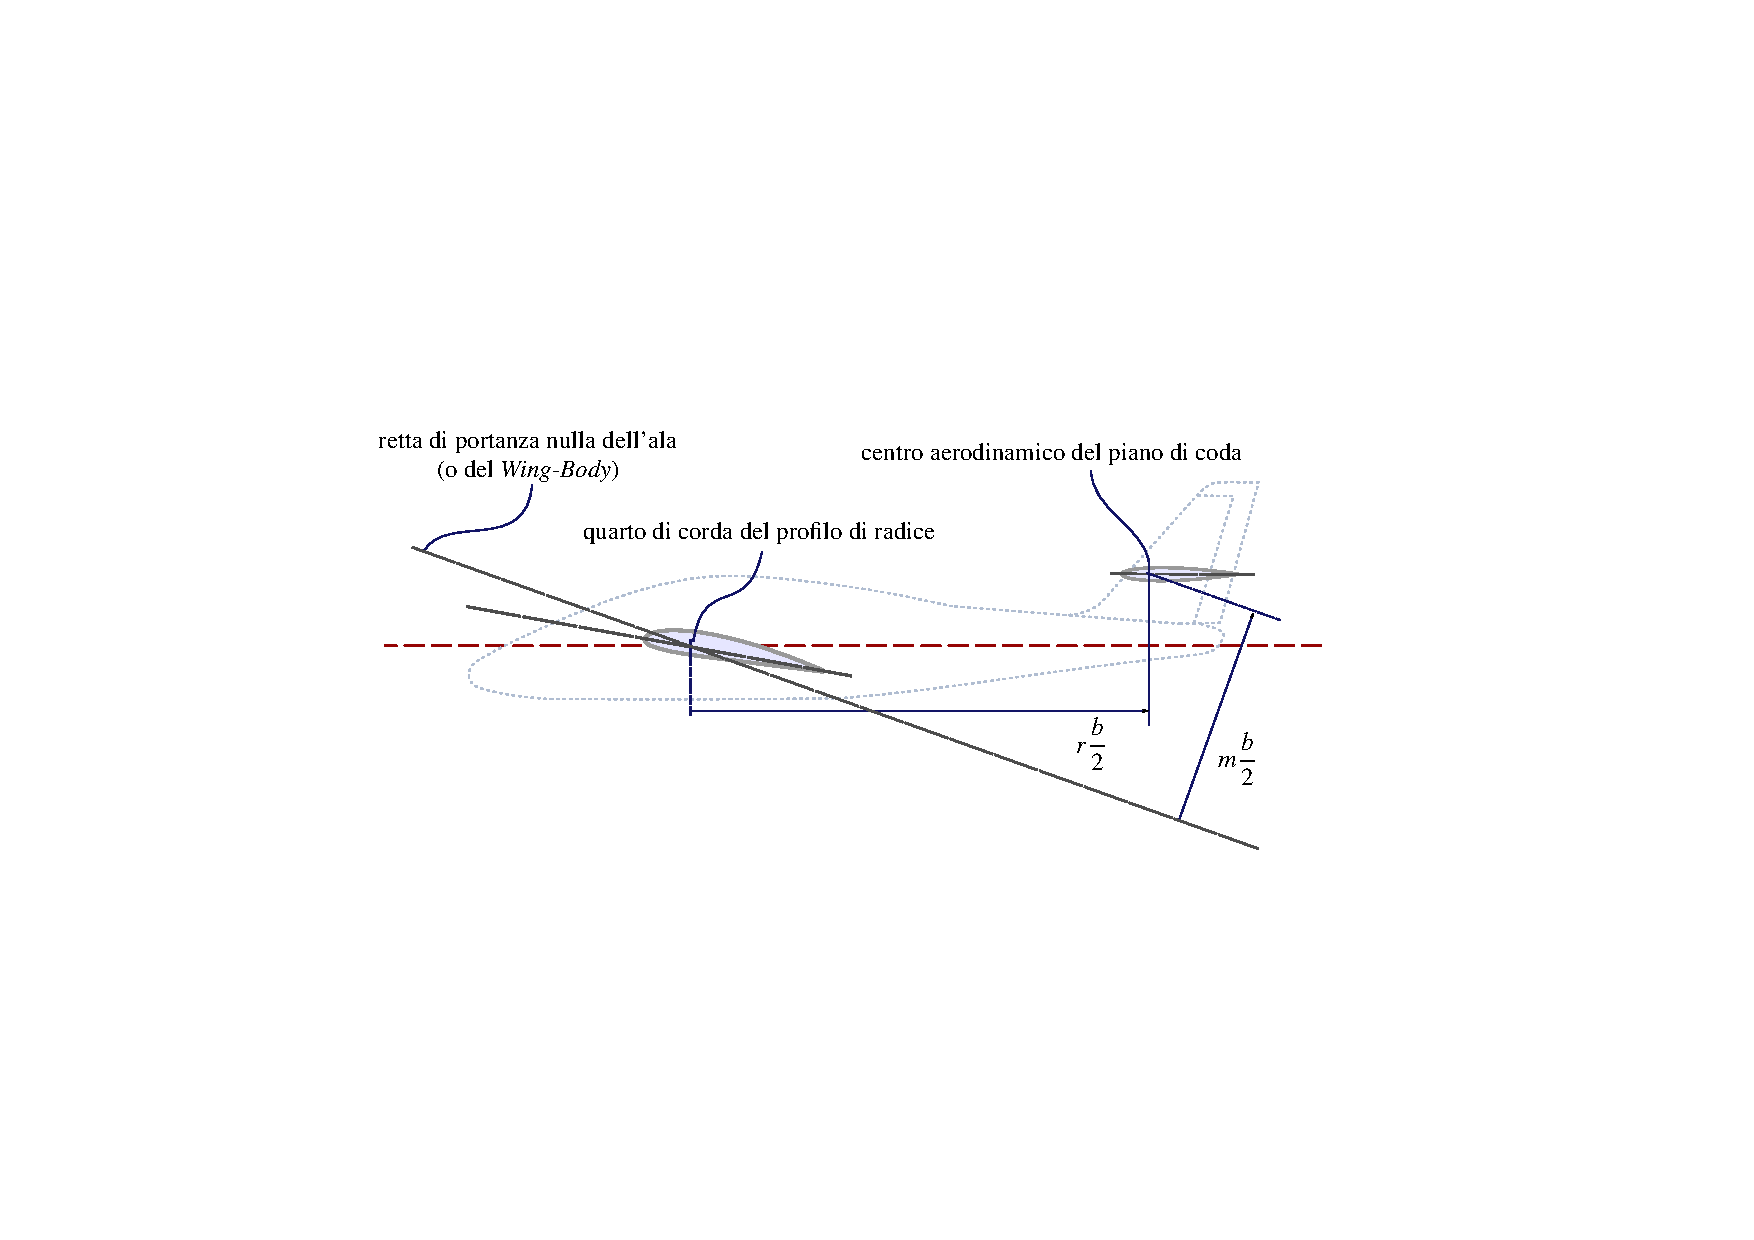
\includegraphics[height=7.3cm]{Immagini/wing_htail_Roskam.pdf}} 
\caption{Dimensions for determination of Downwash Gradient.}
\label{PerkinsDownwash}
\end{figure} 

%% METTI FONTE FORMULA DOWNWASH
%% TODO --> DIVIDI FORMULA \ALIGN
\begin{equation}
 \frac{d\epsilon}{d\alpha} = \frac{K_{\epsilon \Lambda}}{K_{\epsilon _{\Lambda=0}}}  \left ( \frac{r}{r^2+m_{tv}^2} 
 \frac{0.4876}{\sqrt{r^2 + 0.6319 + m_{tv}^2}}  + \displaybreak  \left [1+{ \left ( \frac{r^2}{r^2 + 0.7915 + 5.0734 m_{tv}^2} \right ) }^{0.3113} \right ]     \left \{ 1- \sqrt{\frac{m_{tv}^2}{1+m_{tv}^2}} \right \}     \right )    \frac{C_{L_{{\alpha}_w}}}{\pi \AR}\end{equation}

Where the two $K_{\epsilon}$ terms accounting fot the wing sweep angle effect are defined as follow ( where $\Lambda $ expressed in radians):

\begin{equation}
K_{\epsilon \Lambda} = \frac{ 0.1124 + 0.1265 \Lambda + 0.1766 \Lambda^2}{r^2} + \frac{0.1024}{r} +2
\end{equation}

\begin{equation}
K_{\epsilon _{\Lambda=0}} = \frac{ 0.1124 }{r^2} + \frac{0.1024}{r} +2
\end{equation}

% INTRO
% TEST CLASS
% DEVELOPER GUIDE


\chapter{Aircraft Longitudinal Static Stability}
\label{ch:workobject}
\markboth{Aircraft Longitudinal Static Stability}{}
\begin{flushright}
	{\smaller
		\textit{Citazione\\ citazione}\\
		-- Autore}
\end{flushright}

% introduzione... stabilità, grafici e quali sono tutti i dati che servono
%Nicolai 576
\section{Aerodynamic Lift}
% intro
\subsection{Wing}
\subsection{Fuselage}
\subsection{Horizontal Tail}
The H-tail consists of the stabilizer (fixed or moving) and the elevator (moving) for handling the pitch degree of freedom. The H-tail can be positioned low through the fuselage, in the middle cutting through the V-tail, or at the top of the V-tail to form a T-tail. \cite{kundu}
%nicolai p 283
\subsubsection{Elevator index of effectiveness}
 In order to evaluate the contribution to the longitudinal stability of horizontal tail it's necessary to consider the deflection of the elevator. 
		
\begin{figure}[H]
\centering
{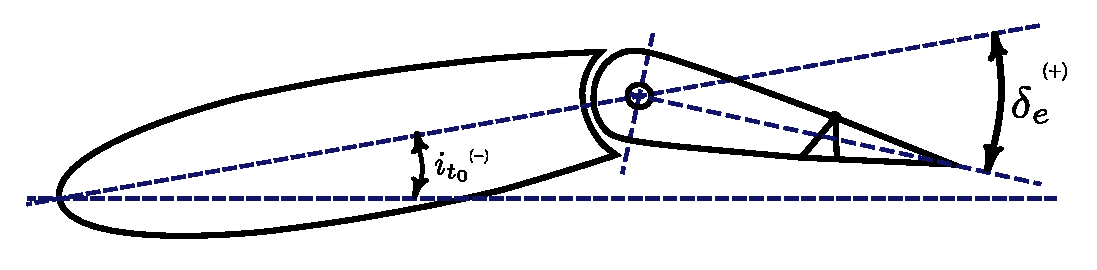
\includegraphics[height=3.09cm]{Immagini/horizontal_tail_profile_deltaE.pdf}} 
\label{htailangle}
\caption{Characteristic angles of the horizontal tail.}
\end{figure} 		
		
The variation of zero lift angle is not constant with the angle of deflection. So it's necessary to evaluate the tau factor which is defined as follows:

\begin{equation}		 
\tau_e = \frac{d \alpha_{0l}}{d \delta_e}
\end{equation}

		
Introducing this parameter the lift coefficient of the horizontal tail can be rated as follows:

\begin{equation}
C_{L_H}= C_{L_0} + C_{L_{{\alpha}_H}} \alpha_H + 	C_{L_{{\alpha}_H}} \tau_e \delta_e
\end{equation}

  
Considering a symmetrical horizontal tail, the term $C_{L_0}$ is zero, so it's possible to express the lift coefficient in the following form:


\begin{equation}
C_{L_H}= C_{L_{{\alpha}_H}} \left ( \alpha_H + \tau_e \delta_e \right)
\end{equation}
  		
 In general the value of $\tau$ is constant until about 15 deg; after this value, due to the flow separation, the effectiveness of elevator decrease and consequently the product $ \tau_e \delta_e$ that appears in the equation of lift coefficient.
		
%grafici di progetto.


\begin{figure}[H]
\centering
{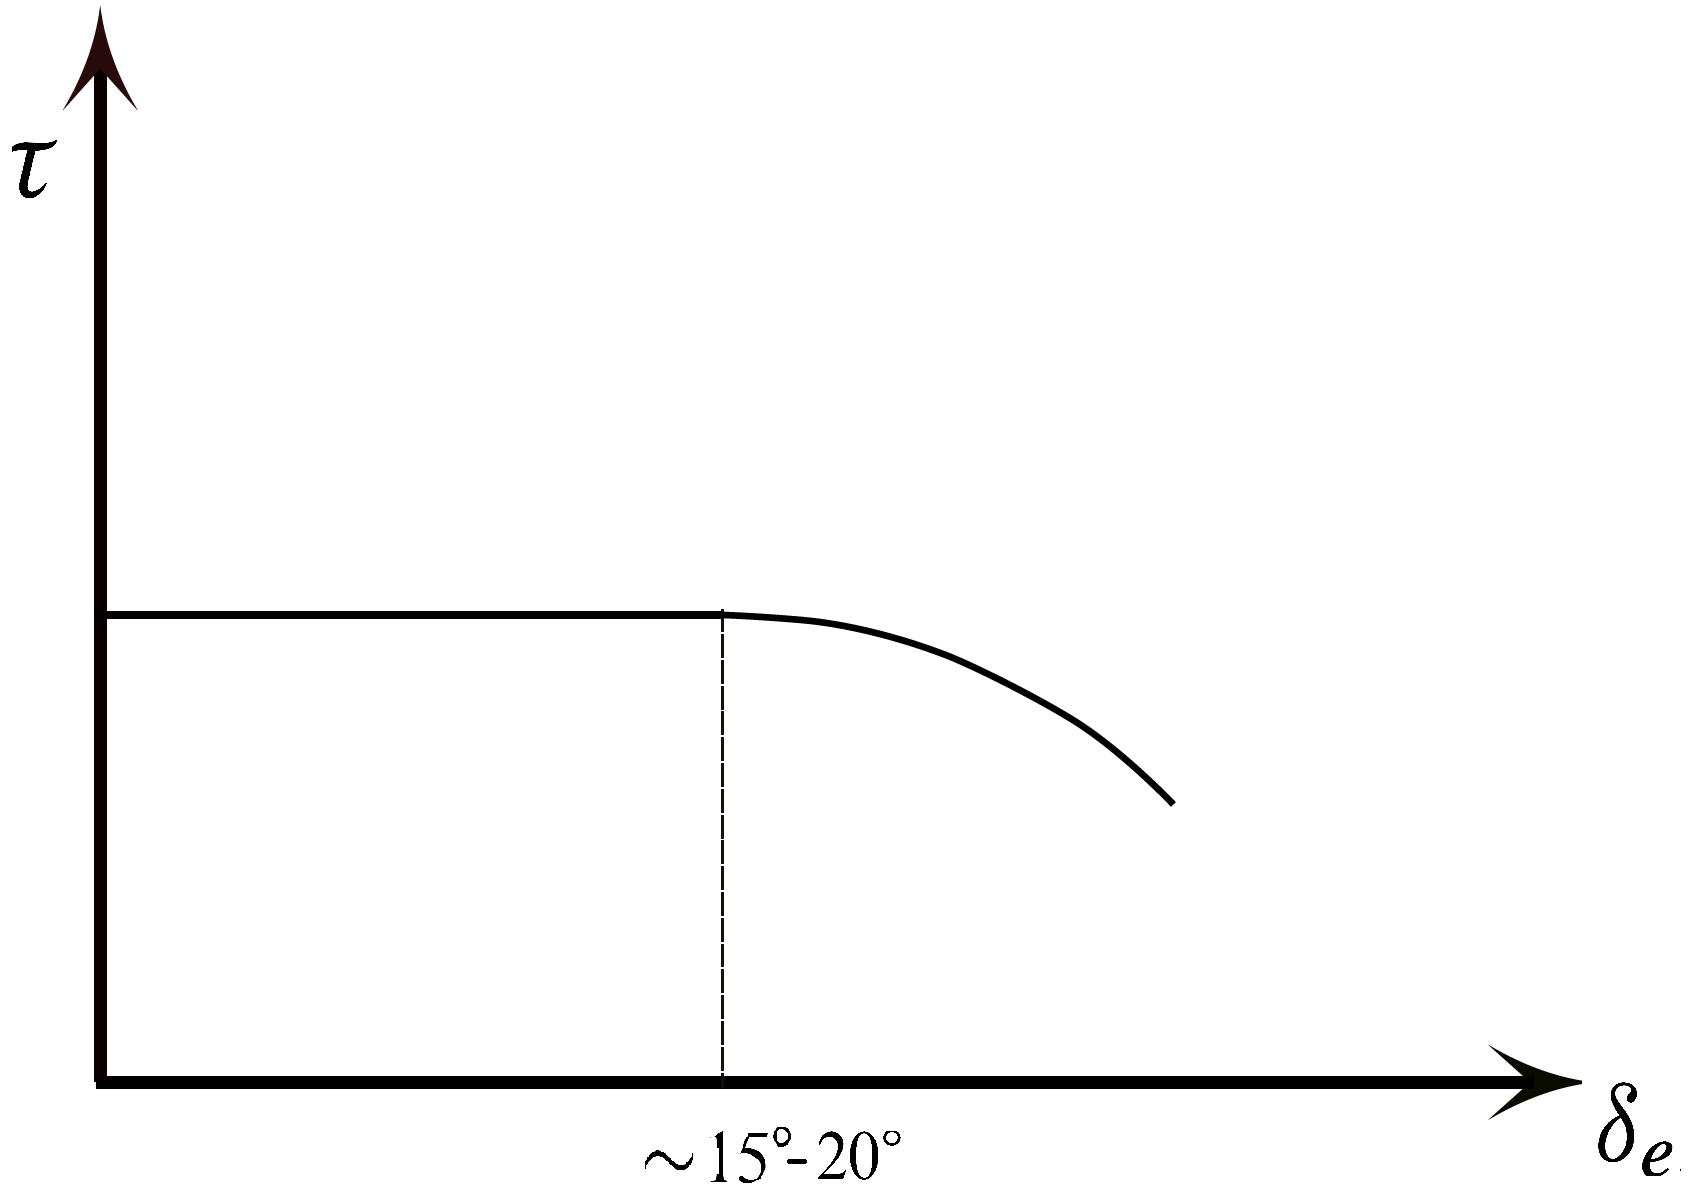
\includegraphics[height=6.79cm]{Immagini/taude.png}} 
\label{tau1}
\caption{Qualitative trend of $\tau$ with the deflection of elevator.}
\end{figure} 		


\begin{figure}[H]
\centering
{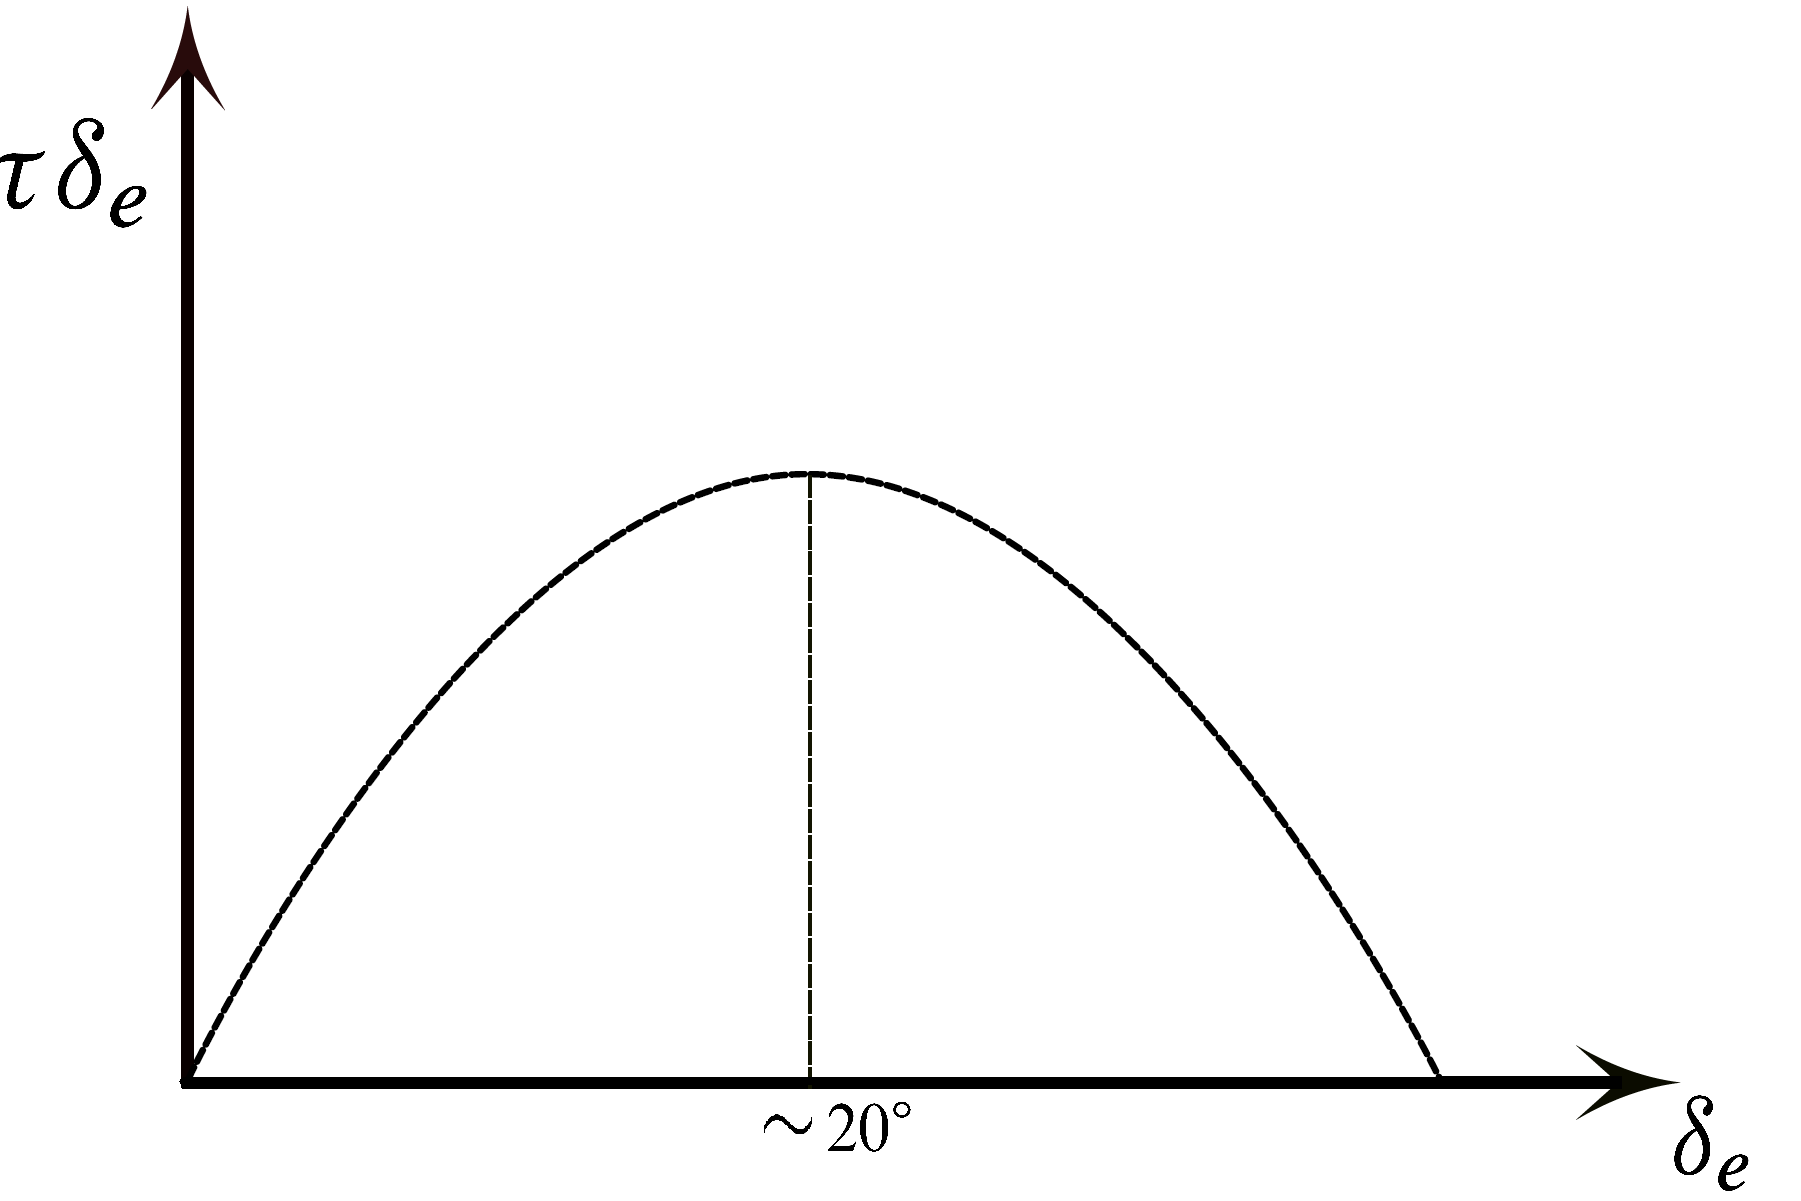
\includegraphics[height=6.79cm]{Immagini/taudeltae.png}} 
\label{tau2}
\caption{Qualitative trend of the term $\tau \cdot \delta_e$ with the deflection of elevator.}
\end{figure} 		


\begin{figure}[H]
\centering
{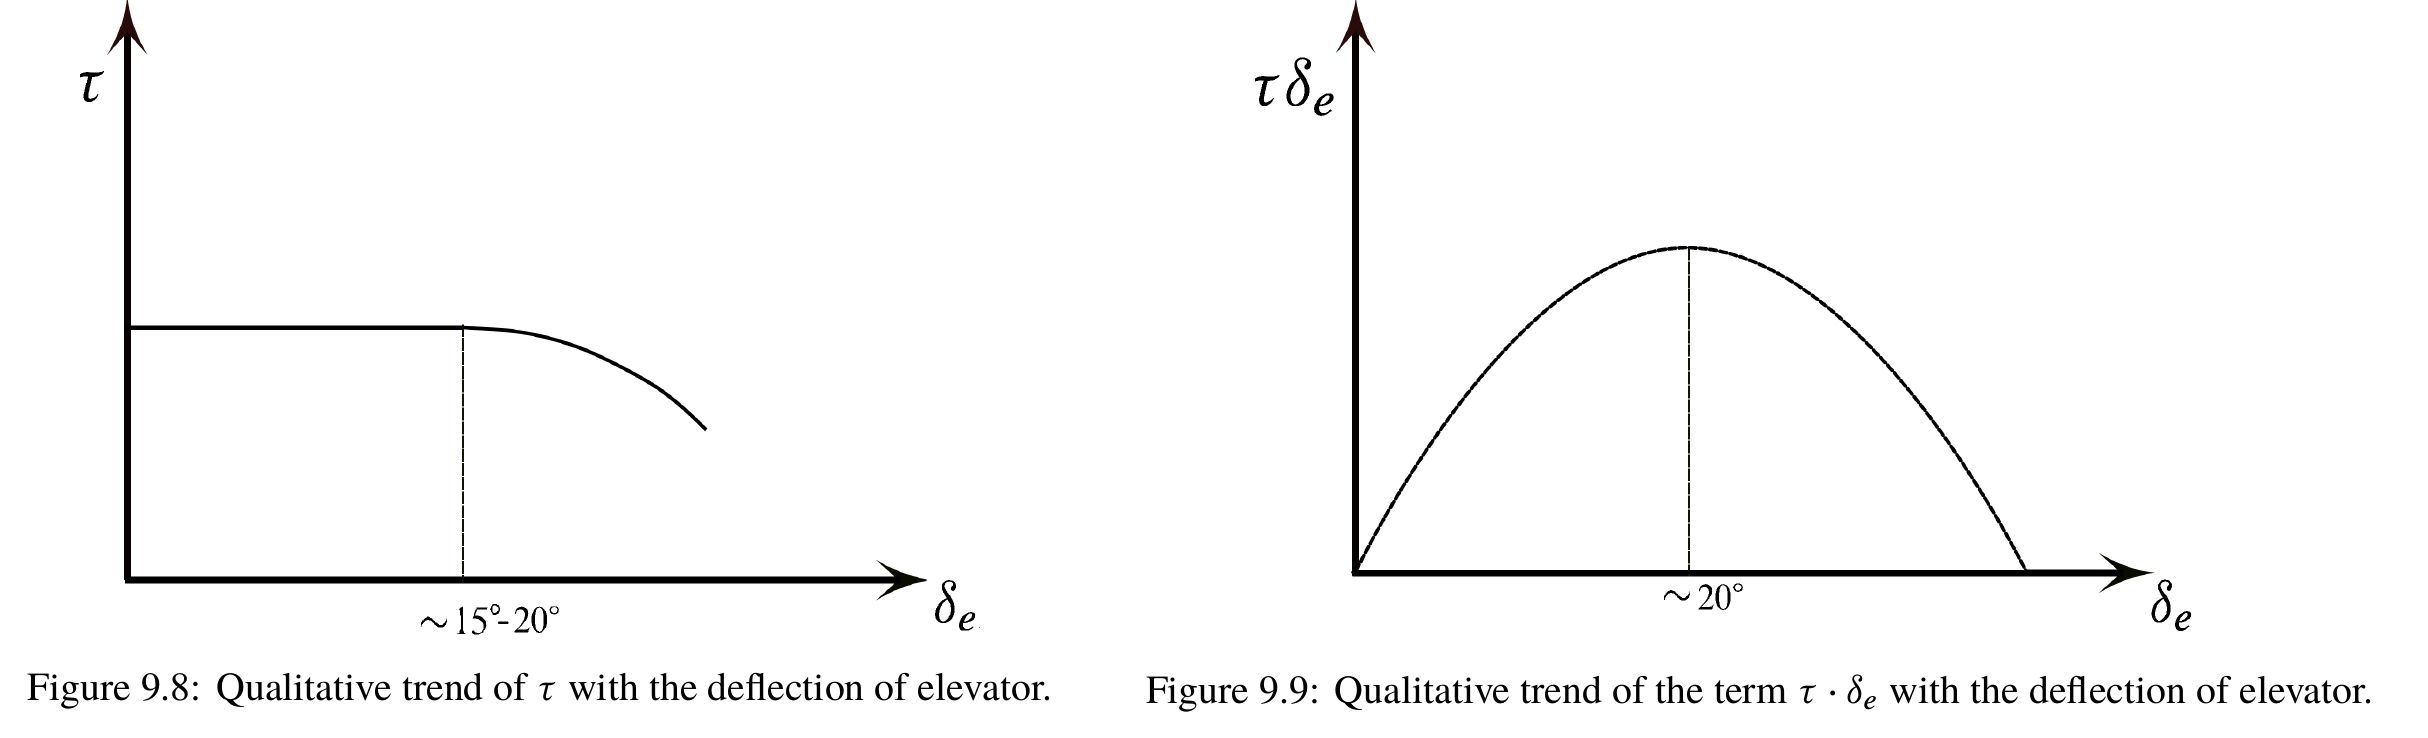
\includegraphics[height=4.9cm]{Immagini/tau.png}} 
\label{tau3}
\end{figure} 		


		
The evaluation of tau is made by reading of external database, considering the following graphs.
	
\begin{equation}
\tau = \alpha_{\delta} \eta_{\delta} = \frac{\alpha_{{\delta}_{c_L}}}{\alpha_{{\delta}_{c_l}}}\alpha_{{\delta}_{c_l}} \eta_{\delta}
\end{equation}



%\begin{figure}[H]
%\centering
%{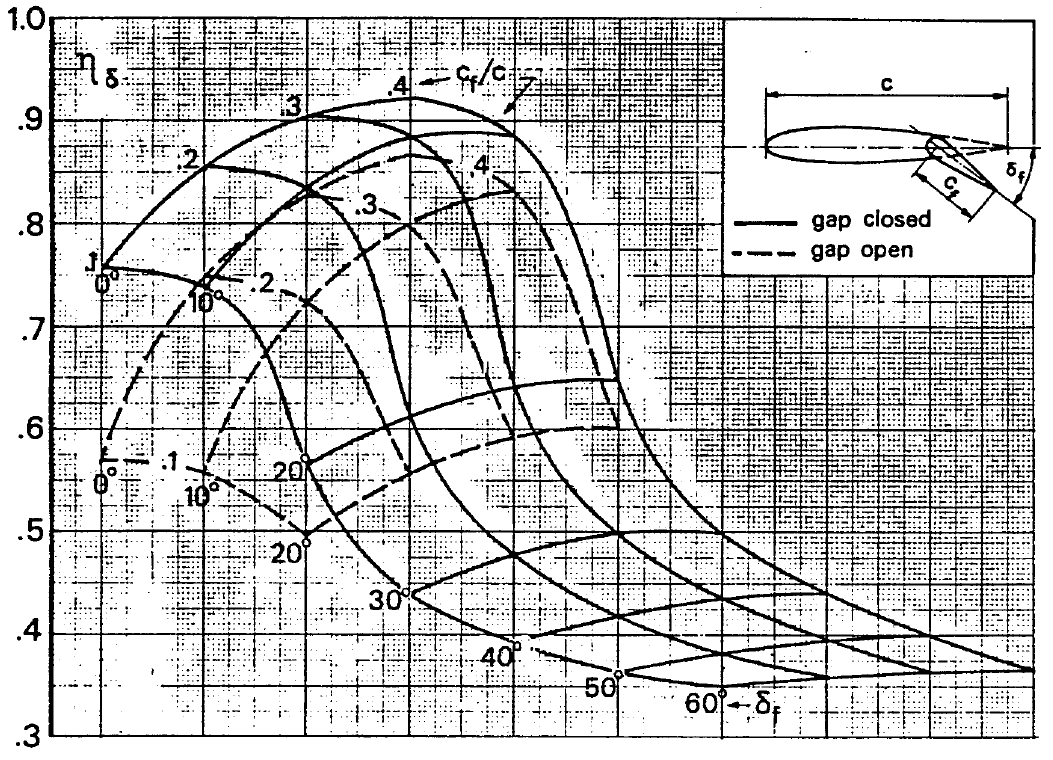
\includegraphics[height=6cm]{Immagini/Eta_Delta_Plain.png}} 
%\caption{2D efficiency correction for elevator.}
%\label{efficiency}
%\end{figure} 		
%
%
%\begin{figure}[H]
%\centering
%{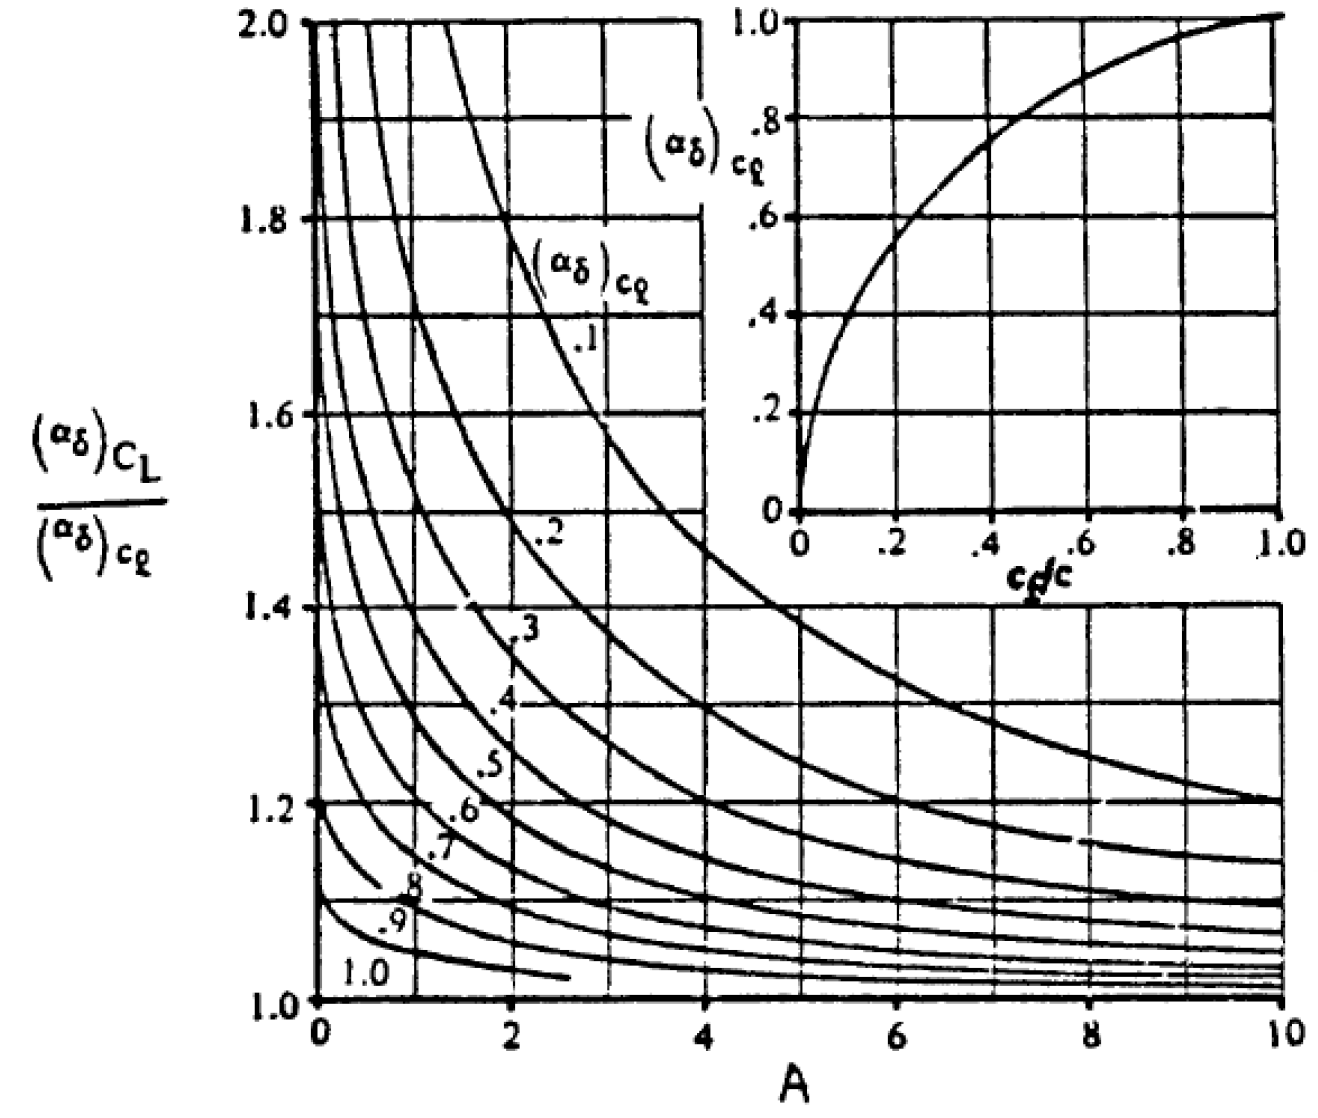
\includegraphics[height=6cm]{Immagini/alfadelta.png}} 
%\caption{$\frac{d \alpha_{0l}}{d \delta_e}$ 2D and 3D correction.}
%\label{efficiency}
%\end{figure} 		

\begin{figure}[H]
\centering
{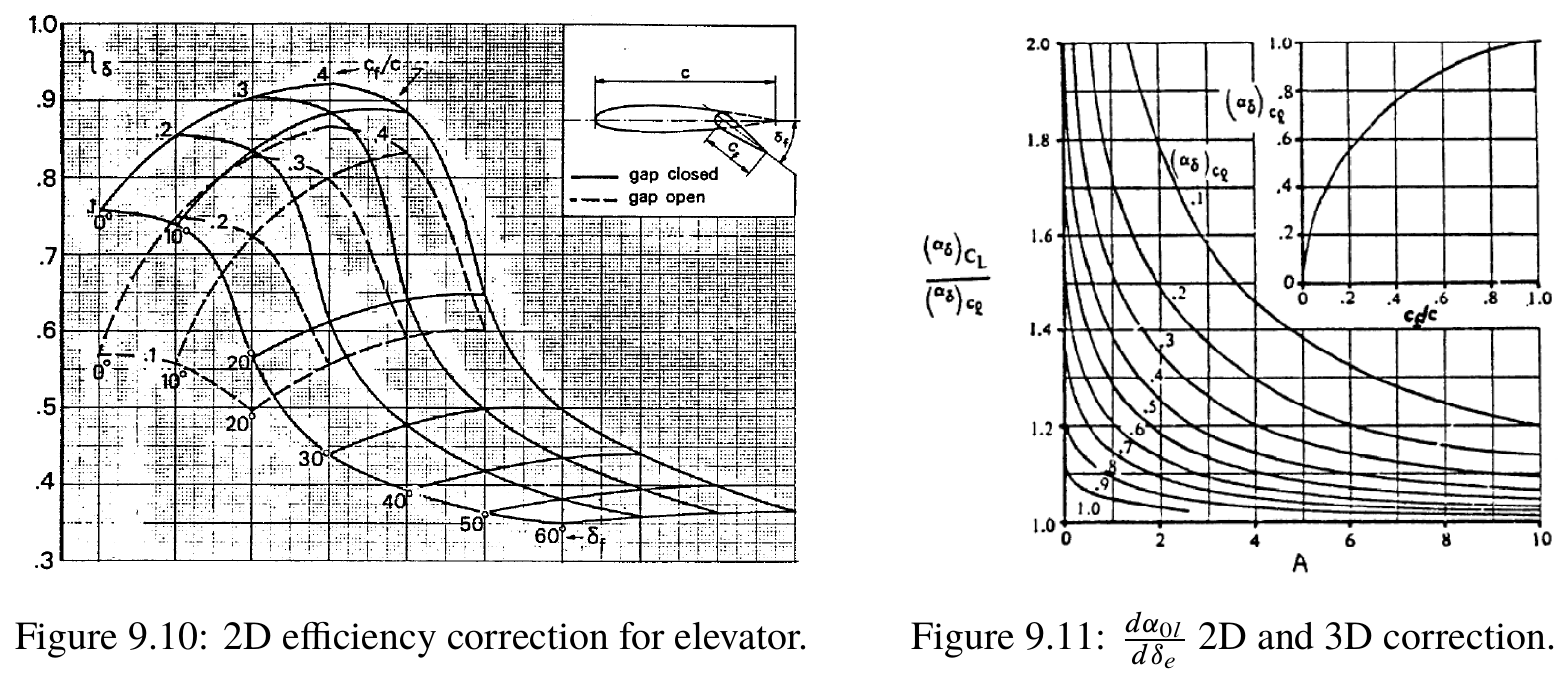
\includegraphics[height=6.79cm]{Immagini/alfadeltanew.png}} 
\label{efficiency}
\end{figure} 		


		
% java class archiecture(?)
%tabella elenco metodi con classe e che fanno

% descrizione

% spiegazione  (da fare) del calcolo del cl at alfa simile a quello dell ala
% spiegazione (da fare )  metodo calcolo tau in stability calculator
% spiegazione (gia fatta) del metodo calculateclwithdeflection in ls aerodynamic

% grafici con risultati

\subsection{Complete Aircraft}

In order to evaluate the lift coefficient of the entire airplane it's possible to consider it as consisting of the following parts\cite{ roskam2002airplane}:

\begin{itemize}
\item Wing and Fuselage
\item Horizontal Tail
\item Canard
\end{itemize}

It's important to consider the effectiveness angles of attack in which the surfaces work. This is made considering the angles of incidence of the lifting surfaces and the downwash angle aft of the wing. An horizontal tail and a canard may be equipped with a trailing edge control surface. So in order to evaluate these contributes it's important to know the angle of deflection $\delta$ of these control surfaces.\\
The calculation of the individual contributions it's reported in the relevant sections. In this section will be shown the method to evaluate the aircraft lift coefficient, known the single contributes.\\
For an aircraft with no canard, the formula is the following:

\begin{equation}
C_L = C_{L_{wb}} + \frac{S_t}{S_w} \eta_t C_{L_{t}}
\end{equation}

Where $\eta_t$ is the ratio of dynamic pressure. In fact the dynamic pressure seen by horizontal tail differ from the free stream dynamic pressure due to two main reasons: the combination wing-fuselage and the presence of the propeller. The dynamic pressure of the tail depends on the location of the tail. If the tail is in the wake of the wing-body, the local dynamic pressure will be less than the freestream because the flow gradually loses its kinetic energy. While if the tail is in the slipstream of propeller, the local dynamic pressure may increase due to the power absorbed by the propeller.



\section{Aerodynamic Drag}
% nell' ottica di questo lavoro divideremo per componente
% foto divisione p 387 sforza pdf
% mettiamo ala piano coda e fusoliera
\subsection{Wing}
\subsection{Fuselage}
\subsection{Horizontal Tail}
% contributo dovuto al flap
\section{Pitching Moments}
\subsection{Wing}
\subsection{Fuselage}
\subsection{Horizontal Tail}
\subsection{Propulsors}

\subsection{Stability Calculation}

% calcolo delle forze normali e tangenziali, calcolo momenti, risultati

\section{Java Class Architecture}
% intro
% riepilogo di tutte le classi in schema. vedi su quaderno  prima di stabilita
% schema in yed

\section{User's Guide}
%intro
% test class

\section{Analysis Results} % fai qui? oppure durante?
%grafici
\chapter{Minor Works}
%\section{Intermediate Airfoil}
%\section{Mean Airfoil}
%The mean airfoil is a representative profile of the wing that owns the mean characteristic of the wing. This is obtained through the influence area of the airfoils as shown in fig. \ref{fig:influencearea}.
%
%\begin{figure}[H]
%\centering
%{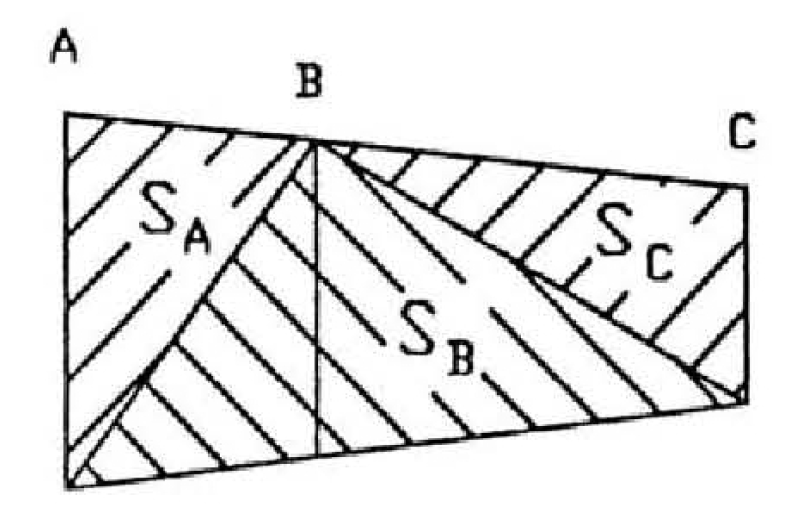
\includegraphics[height=3cm]{Immagini/influencearea}} 
%\caption{Influence area of the sections for finite wing.}
%\label{fig:influencearea}
%\end{figure}
%
%Then is possible to calculate the influence coefficients. 
%
%\begin{equation}
%K_i = \frac{2 S_i}{S}
%\end{equation}
%
%The mean parameters can be obtained from:
%
%\begin{equation}
%\overline{x} = x_1 K_1 + x_2 k_2 +x_3 k_3...
%\end{equation}
%
%In particular, for a wing defined by three airfoils, the end of linearity angle of attack is obtained from the following equation:
%
%\begin{equation}
%\alpha^* = \alpha^*_{1} K_1 + \alpha^*_{2} k_2 +\alpha^*_{3} k_3
%\end{equation}

\begin{flushright}
	{\smaller
		\textit{Once we accept our limits,\\  we go beyond them.}\\
		-- Albert Einstein}
\end{flushright}

\section{Induced Angle of Attack}
When a wing passes through the air, it creates a perturbation, which leads to a vertical component on the relative motion on the air over the wing. Consequently the air flow past the wing is inclined in regard of the initial free stream. Then, the wing behaves as thought the flow were coming from a different direction: the local flow direction.

\begin{figure}[H]
\centering
{\includegraphics[height=3.9cm]{Immagini/induced}} 
\caption{Definitions of induced end effective angles of attack.}
\end{figure}

In practice, these perturbations are generated by the wingtip vortices, which create downwash and deflects the local airflow in the vicinity of the wing downward. This angle is the induced angle of attack $\alpha_i$. The airfoil section itself is then responding to an effective angle of attack equal to the geometric angle of attack minus the induced angle of attack: $\alpha_e=\alpha-\alpha_i$. In most cases, the absolute value of the angle of attack is decreased, and so as for the lift force. Then, in order to produce a given lift force, the AOA of the wing must be greater than the AOA that would be given by a theoretical study of the wing section (2D wing). Moreover, the resulting force exerted by the air on the wing, now perpendicular to the local flow direction, is tilted backwards by an angle equal to the induced angle of attack and then is no longer perpendicular to the free stream velocity. This important phenomenon is at the origin of the induced drag (i.e. the component of the resulting force parallel to the free stream velocity), and therefore for a given lift, a greater induced AOA implies a greater drag. One must bear in mind that because this is a 3-dimentional effect.\cite{induced}\\

In order to evaluate the effective angle of attack  for each spanwise station, it's possible to implement an iterative process in witch at a load distribution it's evaluated the related induced angles that generates a new load distribution.\\
The induced angle of attack is in eq. \ref{eq:alp},  where w is the vertical downwash component:

\begin{equation}
\alpha =\arctan\left( {\frac{w}{V}}\right )
\label{eq:alp}
\end{equation}

\begin{figure}[H]
\centering
{\includegraphics[height=1.6cm]{Immagini/atg}} 
\caption{Geometrical representation of induced angle of attack.}
\end{figure}

The lifting surfaces is considered as divided in several rectangular horse-shoe vortices along the span; one horseshoe vortex along the chord is used, that is, the midpoints of the vortices are placed only at points along the quarter-chord lines. An equal number of control points are located along the three-quarter-chord lines. The velocity from the total vortex system is equated to the component of free-stream velocity normal to the lifting surface chord at each control point.\\
The downwash velocity at any of the control points P, which results from the 2N horseshoe vortices is:

\begin{equation}
w = \frac{1}{4\pi} \sum_{n=1}^N \Gamma_N F'_{w,\nu_N}
\end{equation}

where $\Gamma$ is circulation strength, F is the downwash influence function, N are the vortex point and $\nu$ are the vortex points.\\
In JPAD this effect is calculated in the class \texttt{AlphaEffective}.
% by the method \texttt{calculateAlphaEffective}. 
This method has as output an array of value that indicates the effective angls of attack semi-spanwise using the equations introduced before. In order to evaluate these angles you must have as input the operating conditions. 

\begin{lstlisting}[frame=rbl,caption={{\footnotesize Effective angle of attack Test Class}},label= [style=\bfseries]{Listing}]

// -----------------------------------------------------------------------
// Evaluate effective angle of attack
// -----------------------------------------------------------------------

System.out.println("\n \n-----------------------------------------------------");
System.out.println("STARTING EVALUATE EFFECTIVE ANGLE OF ATTACK ");
System.out.println("-----------------------------------------------------");

double[] alphaEffective;

AlphaEffective theAlphaCalculator = new AlphaEffective(
		theLSAnalysis, theWing, theOperatingConditions);
Amount<javax.measure.quantity.Angle> inputAngle = 
		Amount.valueOf(toRadians(8.), SI.RADIAN);

alphaEffective = theAlphaCalculator.calculateAlphaEffective(inputAngle);

System.out.println("\n \n-----------------------------------------------------");
System.out.println(" alpha --> " + inputAngle);
System.out.println(" alpha effective --> " + Arrays.toString(alphaEffective));

System.out.println("\n \n-----------------------------------------------------");
System.out.println("DONE");
System.out.println("-----------------------------------------------------");

\end{lstlisting}



% -----------------------------------------------------------------------------------------
%                                                                A P P E N D I C I
% -----------------------------------------------------------------------------------------

% some configuration commands by package appendix
\cleardoublepage \phantomsection
\renewcommand{\chaptername}{Appendix}
\renewcommand{\appendixtocname}{Appendices}
\renewcommand{\appendixpagename}{Appendices}
\appendixpage
\noappendicestocpagenum
\addappheadtotoc
%\pagestyle{myAppendixPageStyle}
%
% Here we include the appendix material of the book
%
\begin{appendices}% needs package appendix
\pagestyle{pippo}
%------------------------------------------------------------------------------------------
% Meta-commands for the TeXworks editor
%
% !TeX root = ./Libro_MS.tex
% !TEX encoding = UTF-8
% !TEX program = pdflatex

%%------------------------------------------------------------------------------------------
% Meta-commands for the TeXworks editor
%
% !TeX root = ../Tesi.tex
% !TEX encoding = UTF-8
% !TEX program = pdflatex
%
\chapter{HDF databse creation and reading }
\label{ch:hdf}

\section{Creation of a database using MATLAB}\label{par:Appendix1}
Creation and mangment of an HDF Dataset are very important to handle because they allow to generate resources which are required by a lot of analysis; for example by using this datasets it's possible to implement a new engine type allowing the analysis of the preformance of a new aircraft. 
This feature has not been implemented inside JPAD with the purpose of being able to generate the required resources independently.

For more information regarding the \gls{HDF}, the reader can refer to~\cite{hdf}.

\bigskip
\noindent
First of all it's necessary to have curves of the database that has to be digitized; then, with the use of sotware like \emph{PlotDigitizer}, it's possible to acquire them using a finite number of points chosen by the user.
The output of this procedure is a \emph{.csv} file containing all the copule of points which have been used to digitize the specific curve.

Now the matlab code comes in play to manage these data and to generate the digitized curves and the HDF dataset. 
In the example reported there are four curves defined by points through \emph{PlotDigitizer} which have, firstly, been imported in MATLAB generating four \emph{.mat} files; at this point the code interpolates curves points with cubic splines in order to have more points to plot for each curve.

Finally curves are plotted and the HDF Dataset is populated by using \emph{h5create} and \emph{h5write}; in particular curves points, abscissas and parameterization values are attached to the h5 file through these commands.

\bigskip
\lstset{language=Matlab}
\begin{lstlisting}[caption={MATLAB script for creating the HDF Database}, captionpos=t, tabsize=2]
clc; close all; clear all;

%% Import data
DeltaAlphaCLmax_vs_LambdaLE_dy1p2 = importdata('DeltaAlphaCLmax_vs_LambdaLE_dy1p2.mat');
DeltaAlphaCLmax_vs_LambdaLE_dy2p0 = importdata('DeltaAlphaCLmax_vs_LambdaLE_dy2p0.mat');
DeltaAlphaCLmax_vs_LambdaLE_dy3p0 = importdata('DeltaAlphaCLmax_vs_LambdaLE_dy3p0.mat');
DeltaAlphaCLmax_vs_LambdaLE_dy4p0 = importdata('DeltaAlphaCLmax_vs_LambdaLE_dy4p0.mat');

nPoints = 30;
lambdaLEVector_deg = transpose(linspace(0, 40, nPoints));

%% dy/c = 1.2
smoothingParameter = 0.999999;
DAlphaVsLambdaLESplineStatic_Dy1p2 = csaps( ...
    DeltaAlphaCLmax_vs_LambdaLE_dy1p2(:,1), ...
    DeltaAlphaCLmax_vs_LambdaLE_dy1p2(:,2), ...
    smoothingParameter);
DAlphaVsLambdaLEStatic_Dy1p2 = ppval( ...
    DAlphaVsLambdaLESplineStatic_Dy1p2, ...
    lambdaLEVector_deg);
%% dy/c = 2.0
smoothingParameter = 0.999999; 
DAlphaVsLambdaLESplineStatic_Dy2p0 = csaps( ...
    DeltaAlphaCLmax_vs_LambdaLE_dy2p0(:,1), ...
    DeltaAlphaCLmax_vs_LambdaLE_dy2p0(:,2), ...
    smoothingParameter);
DAlphaVsLambdaLEStatic_Dy2p0 = ppval( ...
    DAlphaVsLambdaLESplineStatic_Dy2p0, ...
    lambdaLEVector_deg);
%% dy/c = 3.0
smoothingParameter =0.999999;
DAlphaVsLambdaLESplineStatic_Dy3p0 = csaps( ...
    DeltaAlphaCLmax_vs_LambdaLE_dy3p0(:,1), ...
    DeltaAlphaCLmax_vs_LambdaLE_dy3p0(:,2), ...
    smoothingParameter);
DAlphaVsLambdaLEStatic_Dy3p0 = ppval( ...
    DAlphaVsLambdaLESplineStatic_Dy3p0, ...
    lambdaLEVector_deg);
%% dy/c = 4.0
smoothingParameter = 0.999999; 
DAlphaVsLambdaLESplineStatic_Dy4p0 = csaps( ...
    DeltaAlphaCLmax_vs_LambdaLE_dy4p0(:,1), ...
    DeltaAlphaCLmax_vs_LambdaLE_dy4p0(:,2), ...
    smoothingParameter);
DAlphaVsLambdaLEStatic_Dy4p0 = ppval( ...
    DAlphaVsLambdaLESplineStatic_Dy4p0, ...
    lambdaLEVector_deg);

%% Plots
figure(1)
plot (lambdaLEVector_deg, DAlphaVsLambdaLEStatic_Dy1p2, '-*b' ... , ...);
hold on;
plot (lambdaLEVector_deg, DAlphaVsLambdaLEStatic_Dy2p0, '-b' ... , ...);
plot (lambdaLEVector_deg, DAlphaVsLambdaLEStatic_Dy3p0, '*b' ... , ...);
plot (lambdaLEVector_deg, DAlphaVsLambdaLEStatic_Dy4p0, 'b' ... , ...);
xlabel('\Lambda_{le} (deg)'); ylabel('\Delta\alpha_{C_{L,max}}');
title('Angle of attack increment for wing maximum lift in subsonic flight');
legend('\Delta y/c = 1.2', '\Delta y/c = 2.0', '\Delta y/c = 3.0','\Delta y/c = 4.0');
axis([0 50 0 9]);
grid on;
 
%% preparing output to HDF
% dy/c
dyVector = [1.2;2.0;3.0;4.0];
%columns --> curves
myData = [ ...
        DAlphaVsLambdaLEStatic_Dy1p2, ...
        DAlphaVsLambdaLEStatic_Dy2p0, ...
        DAlphaVsLambdaLEStatic_Dy3p0, ... 
        DAlphaVsLambdaLEStatic_Dy4p0];   

hdfFileName = 'DAlphaVsLambdaLEVsDy.h5';
if ( exist(hdfFileName, 'file') )
    fprintf('file %s exists, deleting and creating a new one\n', hdfFileName);
    delete(hdfFileName)
else
    fprintf('Creating new file %s\n', hdfFileName);
end
% Dataset: data
h5create(hdfFileName, '/DAlphaVsLambdaLEVsDy/data', size(myData'));
h5write(hdfFileName, '/DAlphaVsLambdaLEVsDy/data', myData');
% Dataset: var_0
h5create(hdfFileName, '/DAlphaVsLambdaLEVsDy/var_0', size(dyVector'));
h5write(hdfFileName, '/DAlphaVsLambdaLEVsDy/var_0', dyVector');
% Dataset: var_1
h5create(hdfFileName, '/DAlphaVsLambdaLEVsDy/var_1', size(lambdaLEVector_deg'));
h5write(hdfFileName, '/DAlphaVsLambdaLEVsDy/var_1', lambdaLEVector_deg');
\end{lstlisting}

\bigskip
\begin{figure}[!hb]
\centering
\includegraphics[keepaspectratio, width=0.88\textwidth]{HDF_Dataset_creation.png}
\caption{Flowchart of an HDF Database creation}
\end{figure}

\clearpage
\begin{figure}
\centering
\includegraphics[keepaspectratio, width=0.55\textwidth]{deltaAlphaSforza.png}\includegraphics[keepaspectratio, width=0.55\textwidth]{DAlphaVsLambdaLEVsDy_MATLAB.png}
\caption{Comparison between the initial graph and the digitized one}
\end{figure}

\section{Reading data from an HDF database in JPAD}\label{par:Appendix2}
After creating the database, this has to be read in order to obtain the required data; inside JPAD this operation can be done defining a specific class, which extends the abstract class \lstinline[language=Java]!DatabaseReader! that is designed for HDF dataset reading. 

This son class has a specific structure which main key points can be summarized in the following ones:

\begin{enumerate}
\item Creation of variables, in number equal to the function to be interpolated, using the type \lstinline[language=Java]!MyInterpolatingFunction! 
\item Creation of variables for all values that are wanted to be read from the interpolating functions
\item Creation of a constructor that accepts the folder path string and the file name string of the database. This constructor has to launch the interpolating method for all functions contained into the database by using  \lstinline[language=Java]!MyInterpolatingFunction! methods.
\item Creation of a getter method for each of the variables allocated at point 2 in order to obtain values from interpolated functions by giving in input the required parameters
\end{enumerate}

\noindent
In particular the class \lstinline[language=Java]!MyInterpolatingFunction! implements methods for a spline, bicubic and tricubic data interpolation as well as three methods for extracting a specific value from each of the previou interpolated curve.

\bigskip
\noindent
The following listing describes, with an example upon the aerodynamic database, how the reader class should be built up following the previous steps.

\lstset{language=Java}
\begin{lstlisting}[caption={DatabaseReader son class creation}, captionpos=t, tabsize=2]
public class AerodynamicDatabaseReader extends DatabaseReader {
// STEP 1:
	private MyInterpolatingFunction 
					c_m0_b_k2_minus_k1_vs_FFR,
					ar_v_eff_c2_vs_Z_h_over_b_v_x_ac_h_v_over_c_bar_v;
// STEP 2:
	double cM0_b_k2_minus_k1, ar_v_eff_c2;
// STEP 3:
	public AerodynamicDatabaseReader(String databaseFolderPath, String databaseFileName) {
		super(databaseFolderPath, databaseFileName);

		c_m0_b_k2_minus_k1_vs_FFR = 
						database.interpolate1DFromDatasetFunction(
										"(C_m0_b)_k2_minus_k1_vs_FFR"
						);
		ar_v_eff_c2_vs_Z_h_over_b_v_x_ac_h_v_over_c_bar_v =
						database.interpolate2DFromDatasetFunction(
										"(AR_v_eff)_c2_vs_Z_h_over_b_v_(x_ac_h--v_over_c_bar_v)"
										);
	}
// STEP 4:	
	public double get_C_m0_b_k2_minus_k1_vs_FFR(double length, double diameter) { 
		return c_m0_b_k2_minus_k1_vs_FFR.value(length/diameter);
	}
// STEP 4:
	public double get_AR_v_eff_c2_vs_Z_h_over_b_v_x_ac_h_v_over_c_bar_v(double zH, double bV, double xACHV, double cV) {
		return ar_v_eff_c2_vs_Z_h_over_b_v_x_ac_h_v_over_c_bar_v.value(zH/bV, xACHV/cV);
	}
}
\end{lstlisting}

\bigskip
\noindent
Once the class is created, is possible to create an object of it in any test class in order to have access to all its methods; in particular the user needs to invoke the getter related to the quantity he wants to read from the interpolating function. 



%
\end{appendices}


\backmatter % materiale finale( bibliografia, risorse utilizzate)



% -----------------------------------------------------------------------------------------
%                                                                L I S T A   D E I   S I M B O L I   E   G L O S S A R I O 
% -----------------------------------------------------------------------------------------
\glsaddall
\glossarystyle{list}
\markboth{}{}
\cleardoublepage
\pagestyle{pippo}
\printglossary[type=main]

\markboth{}{}
\cleardoublepage
\pagestyle{pippo}
\printglossary[type=\acronymtype]

\markboth{}{}
\cleardoublepage
\pagestyle{pippo}
\printglossary[type=symbols]

\newpage
\thispagestyle{empty}
% -----------------------------------------------------------------------------------------
%                                                               A C R O N I M I 
% -----------------------------------------------------------------------------------------

% -----------------------------------------------------------------------------------------
%                                                               B I B L I O G R A F I A
% -----------------------------------------------------------------------------------------

\cleardoublepage \phantomsection
\addcontentsline{toc}{chapter}{Bibliography}
\nocite{*}
%\printbibheading[title={Bibliography}]
\printbibliography[heading=myBibliography]% needs biblatex, see myBibliography in _preamble.tex

\end{document}